The unblinded distributions of BDT outputs are shown in Fig.~\ref{fig:bdt_outputs}.
The pre-fit distributions in the final binning used in the signal extraction are shown in Fig.~\ref{fig:finalbins}, with the post-fit distributions shown in Fig.~\ref{fig:postfit}.
\begin{figure} [!h]
 \centering
 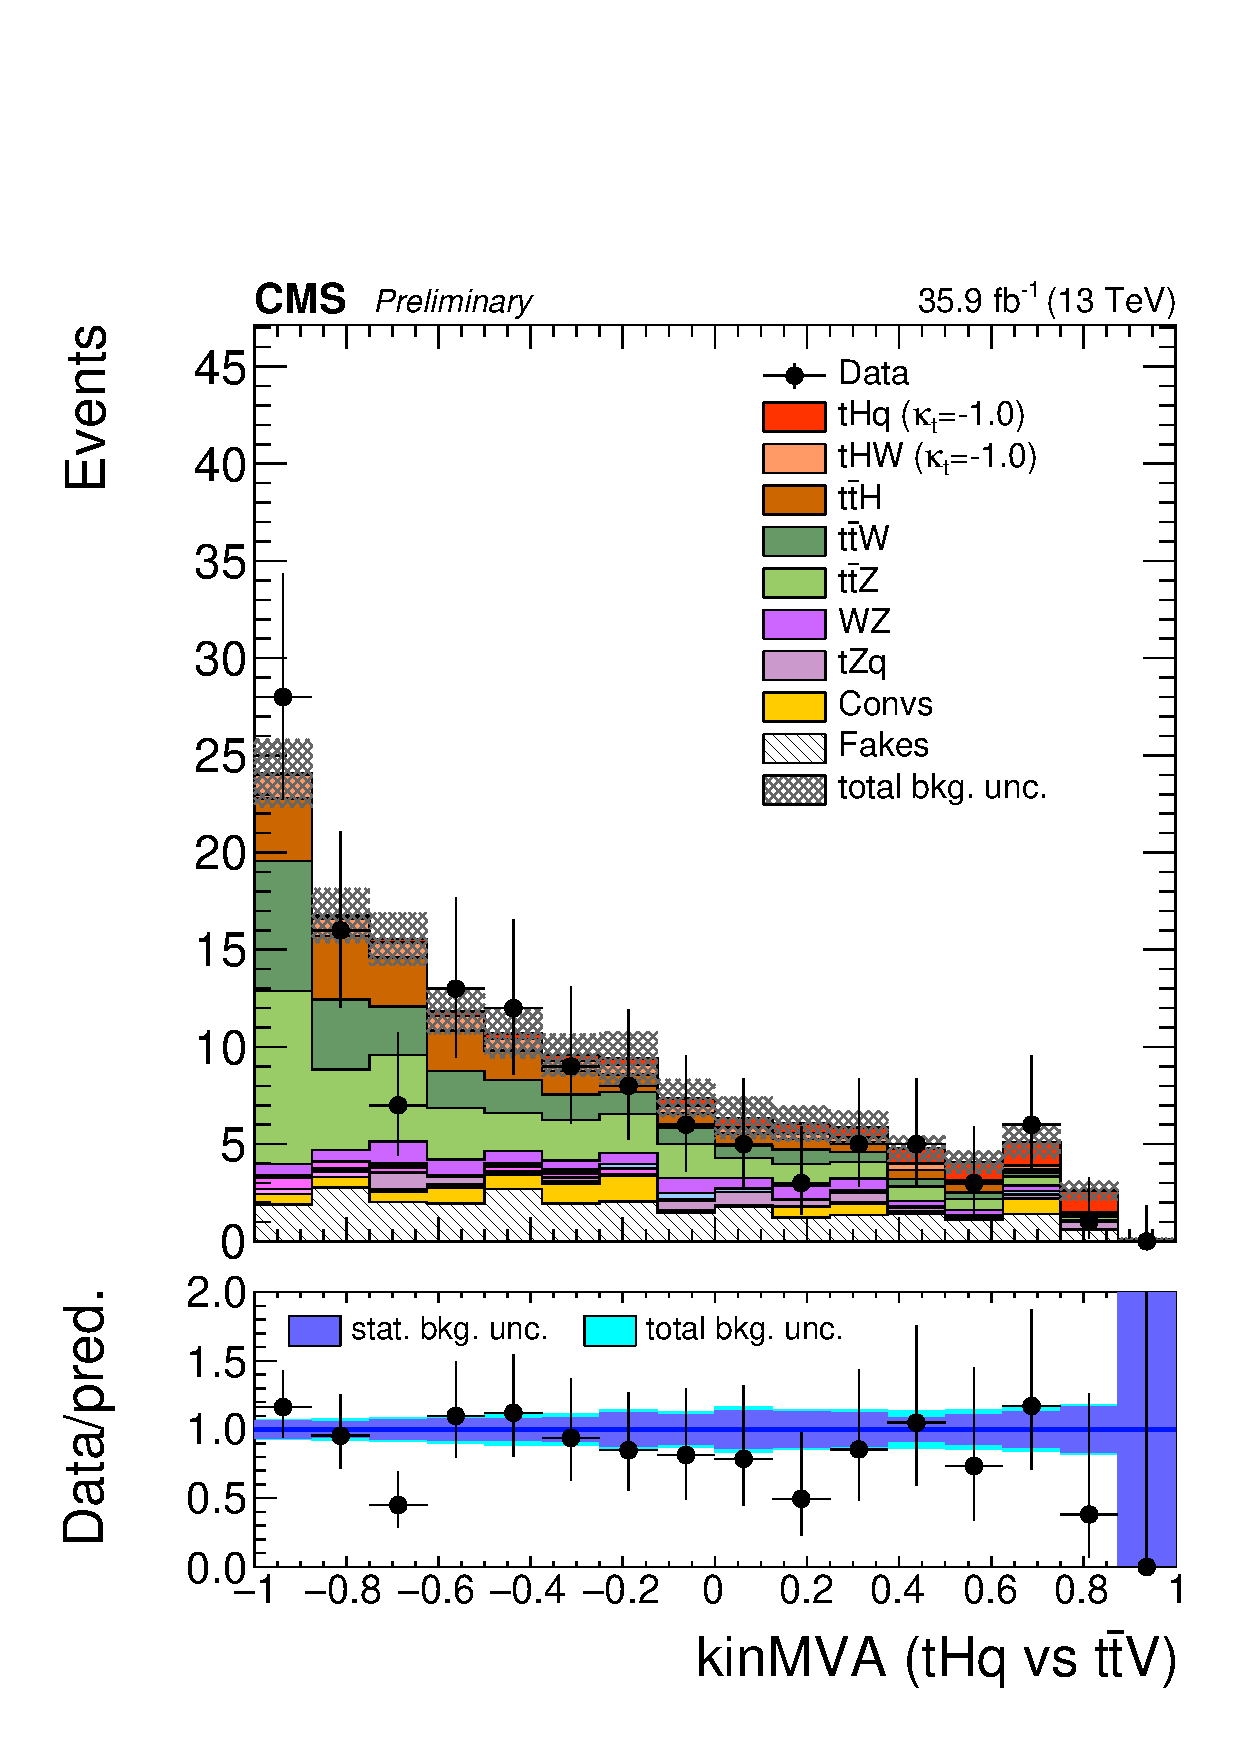
\includegraphics[width=0.32\textwidth]{figures/3lsignal/thqMVA_ttv_3l_40.pdf}
 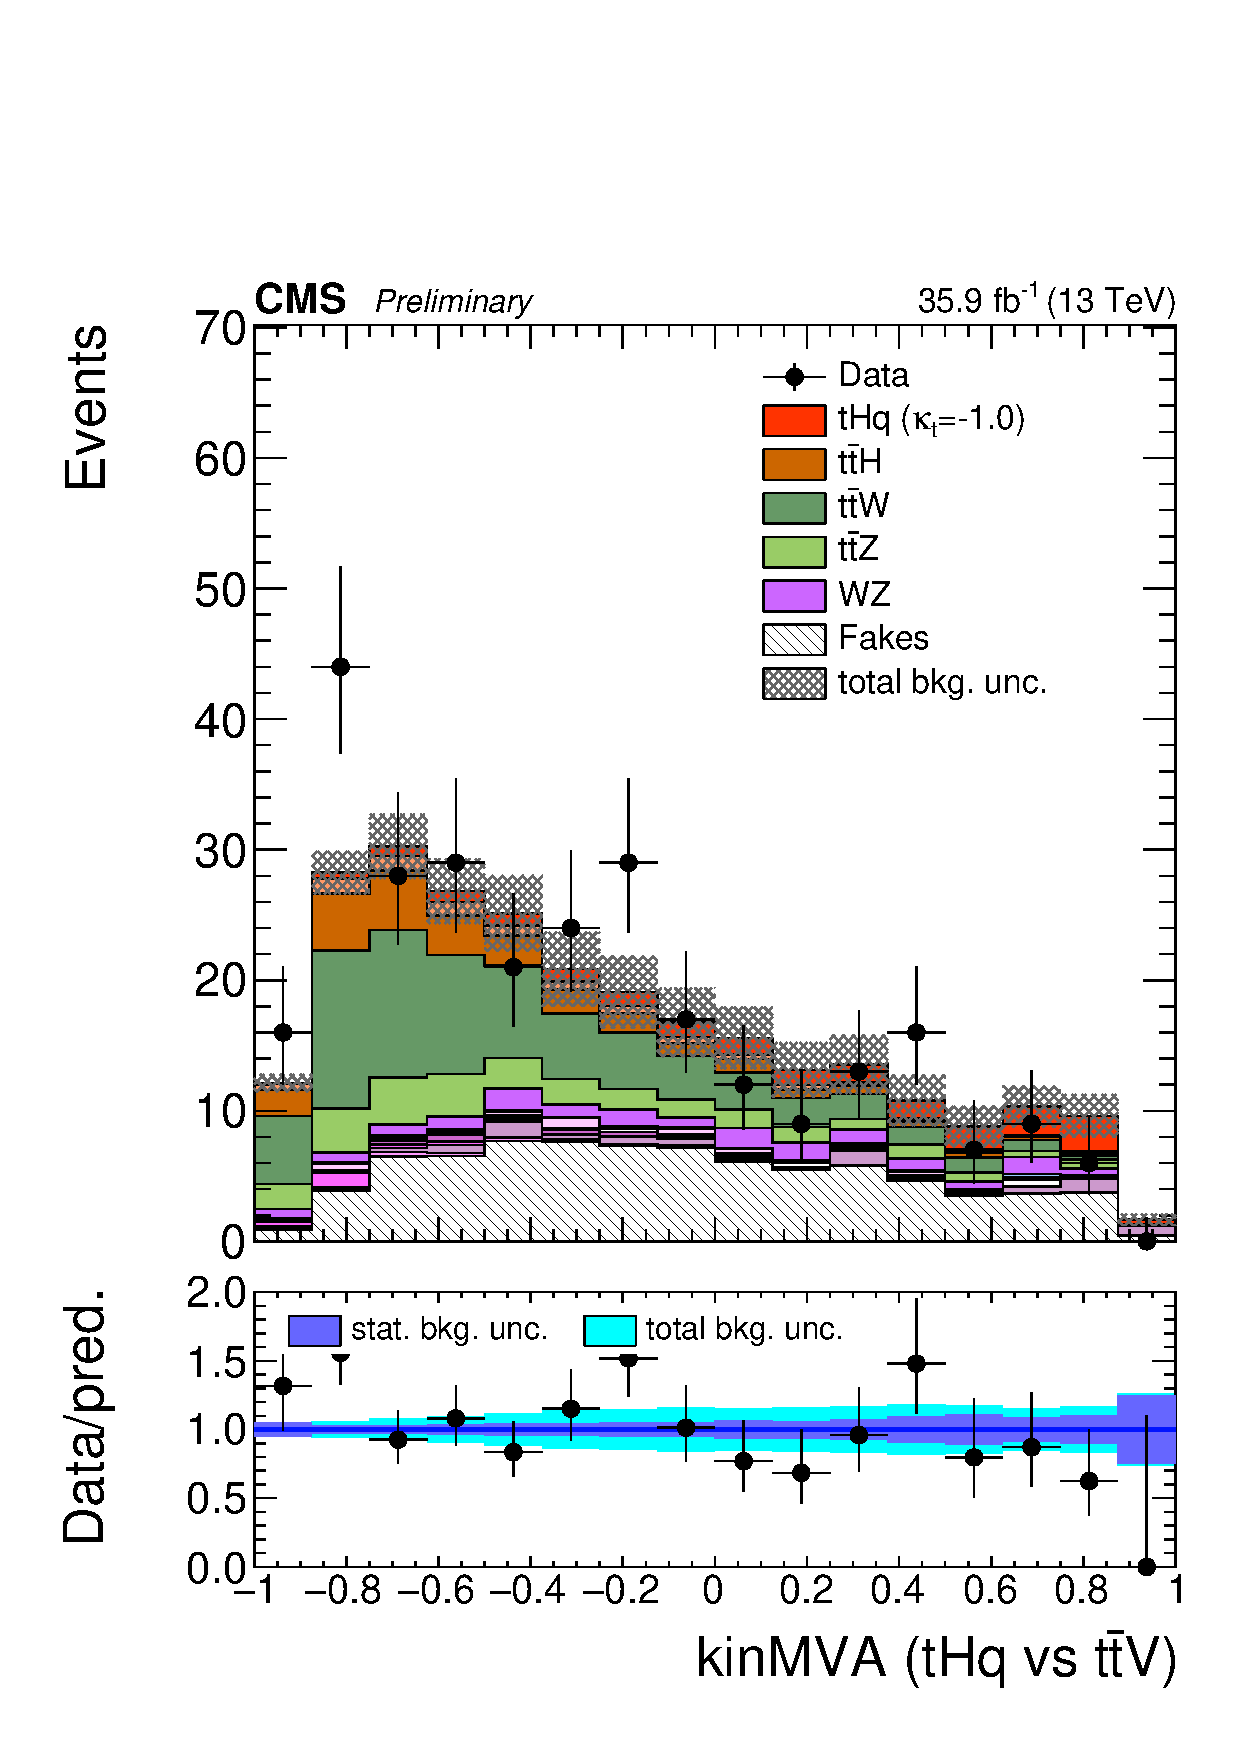
\includegraphics[width=0.32\textwidth]{figures/signalregion_2lss/mumu/thqMVA_ttv_2lss_40.pdf}
 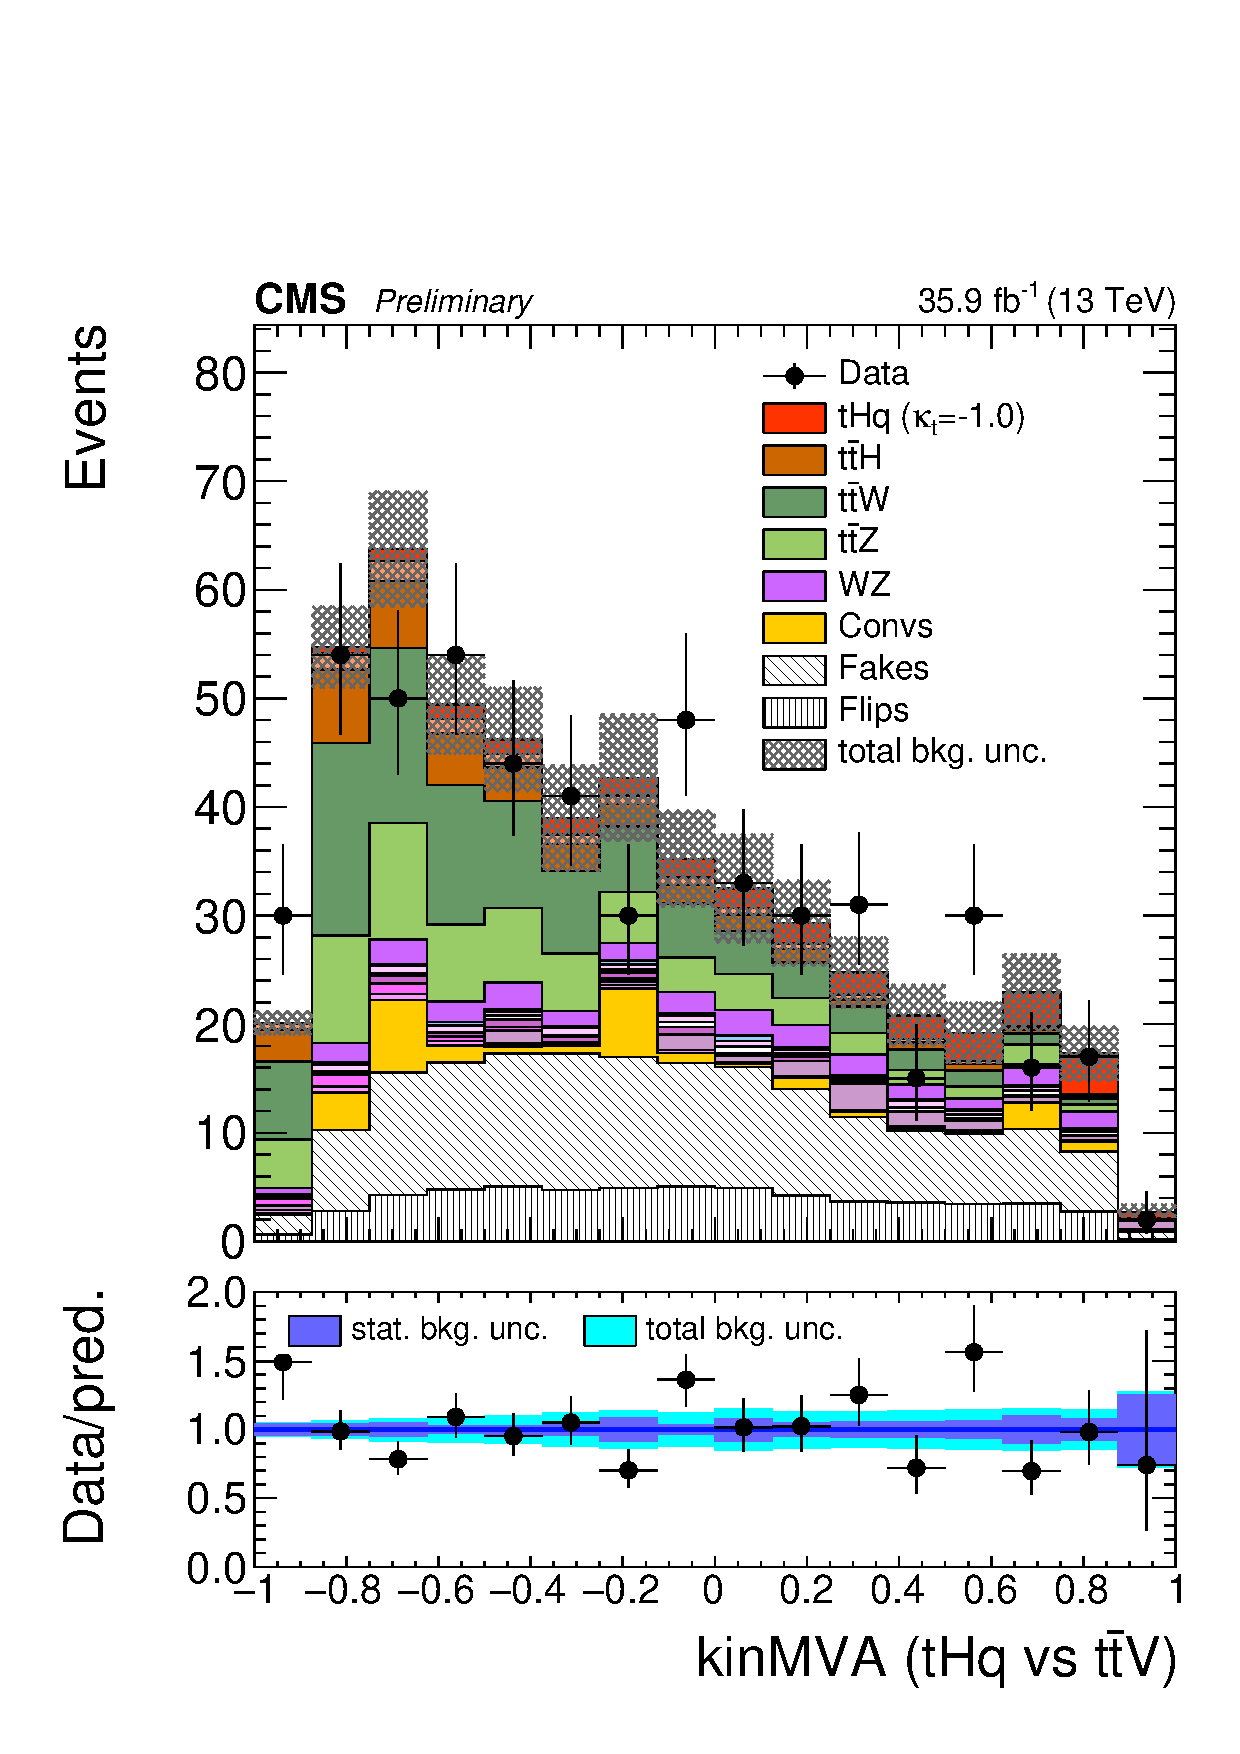
\includegraphics[width=0.32\textwidth]{figures/signalregion_2lss/emu/thqMVA_ttv_2lss_40.pdf} \\
 % 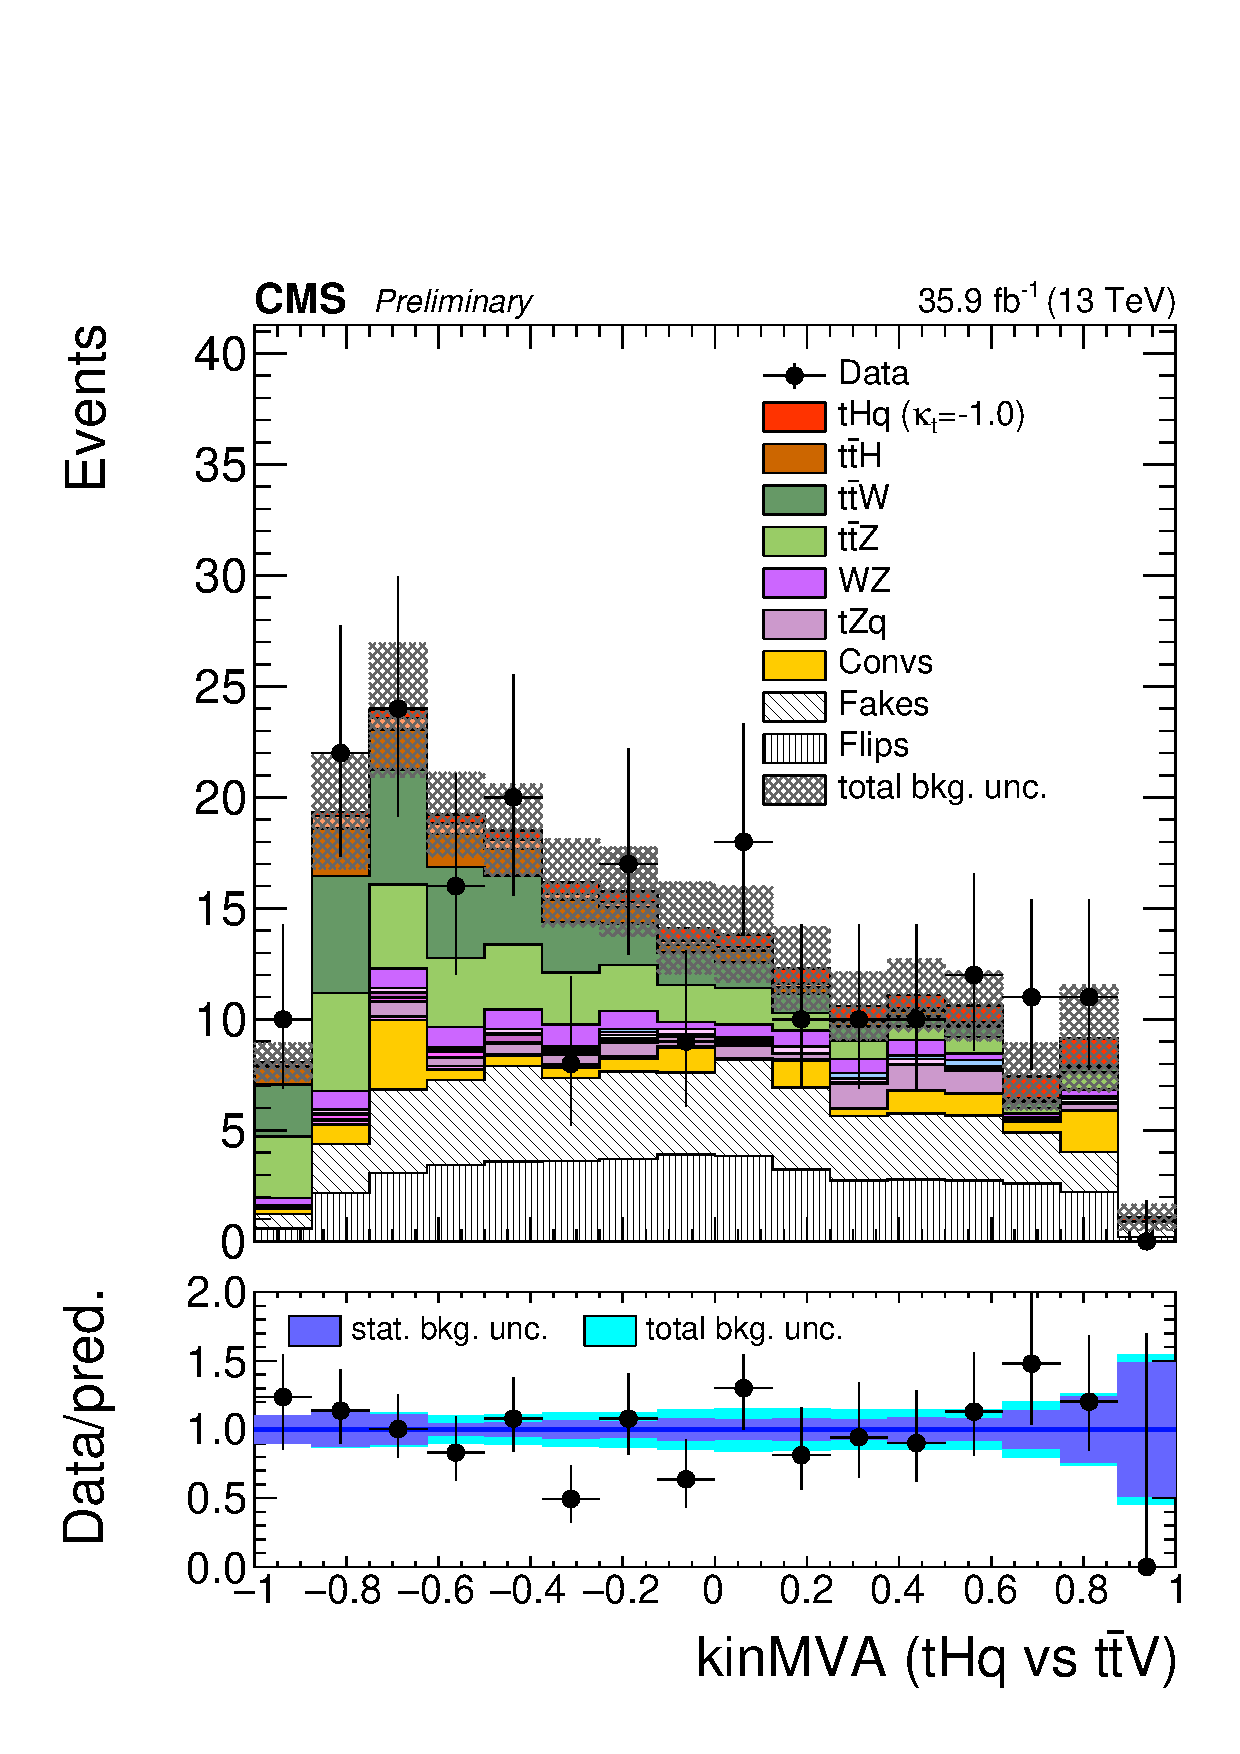
\includegraphics[width=0.24\textwidth]{figures/signalregion_2lss/ee/thqMVA_ttv_2lss_40.pdf} \\
 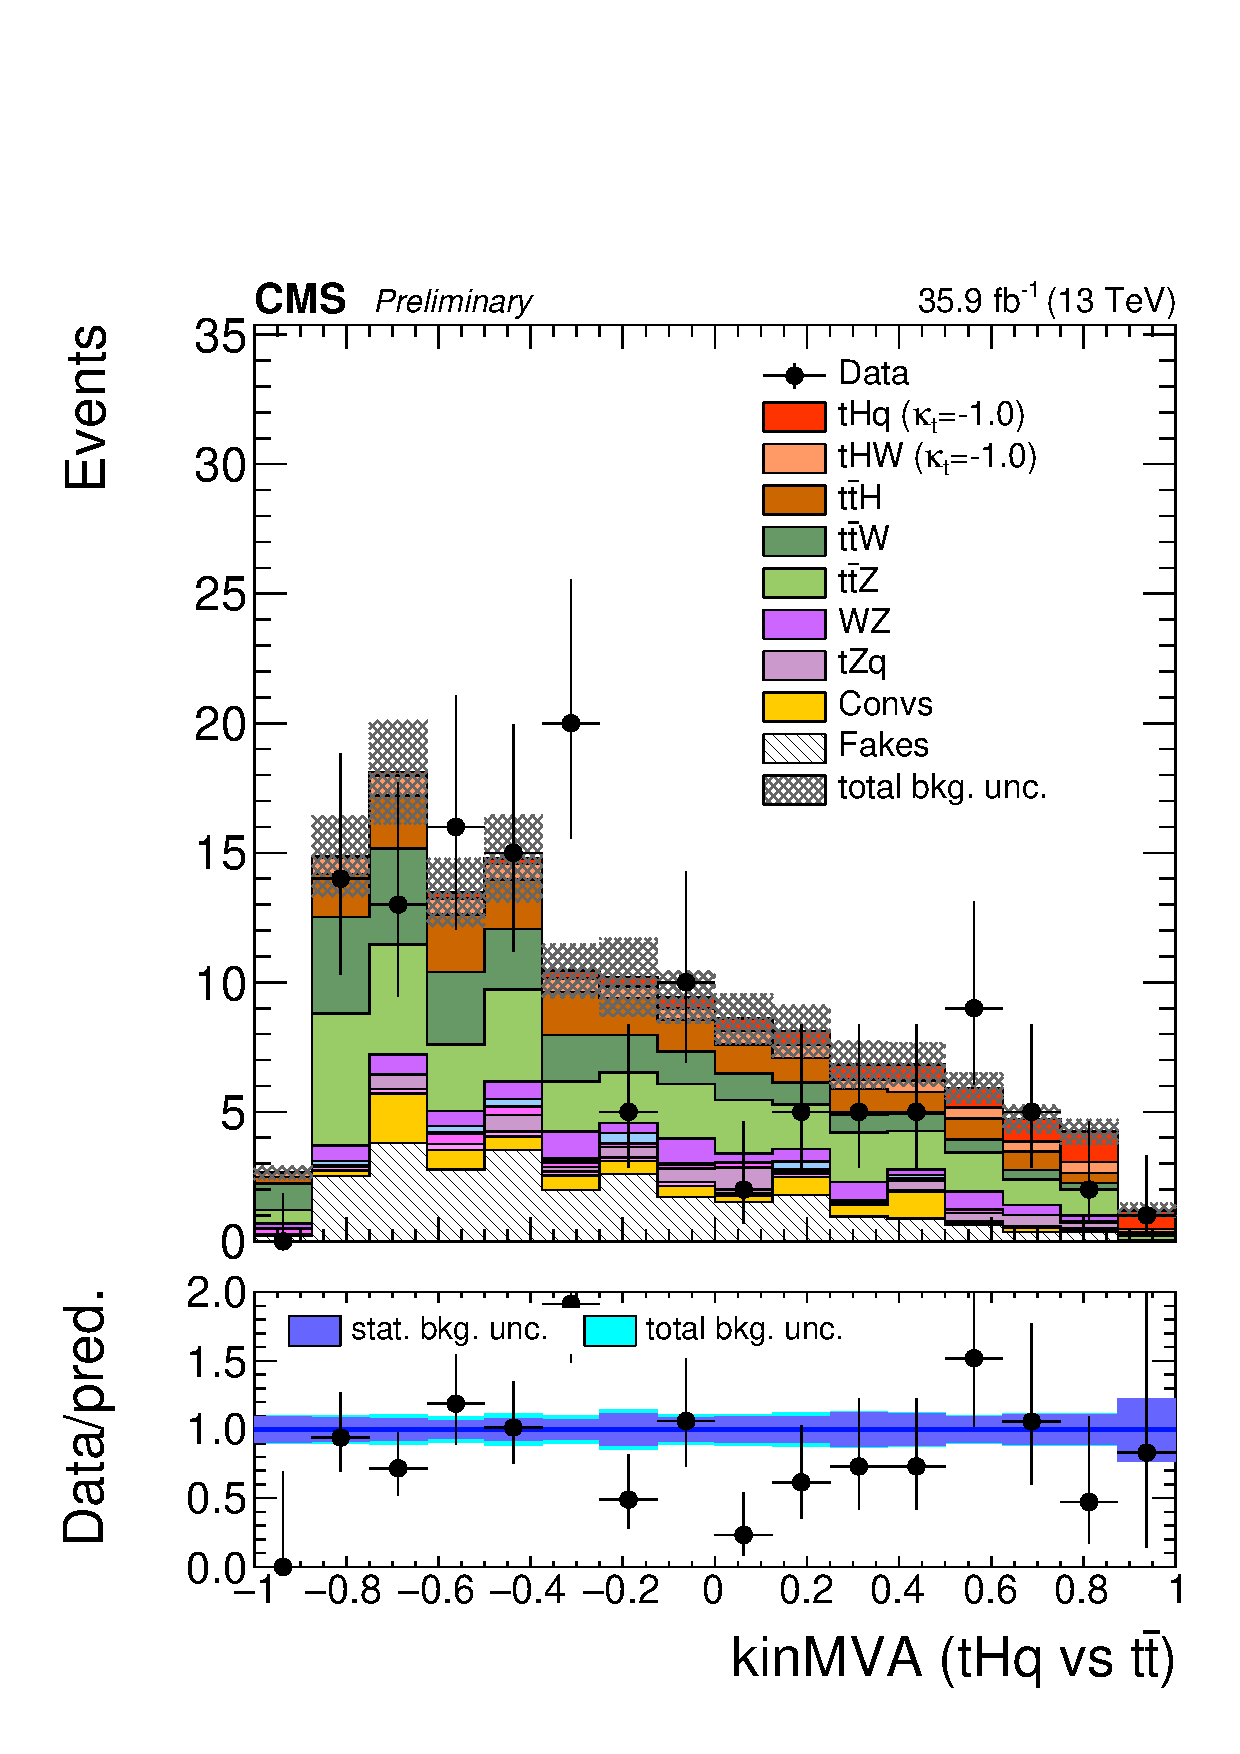
\includegraphics[width=0.32\textwidth]{figures/3lsignal/thqMVA_tt_3l_40.pdf} 
 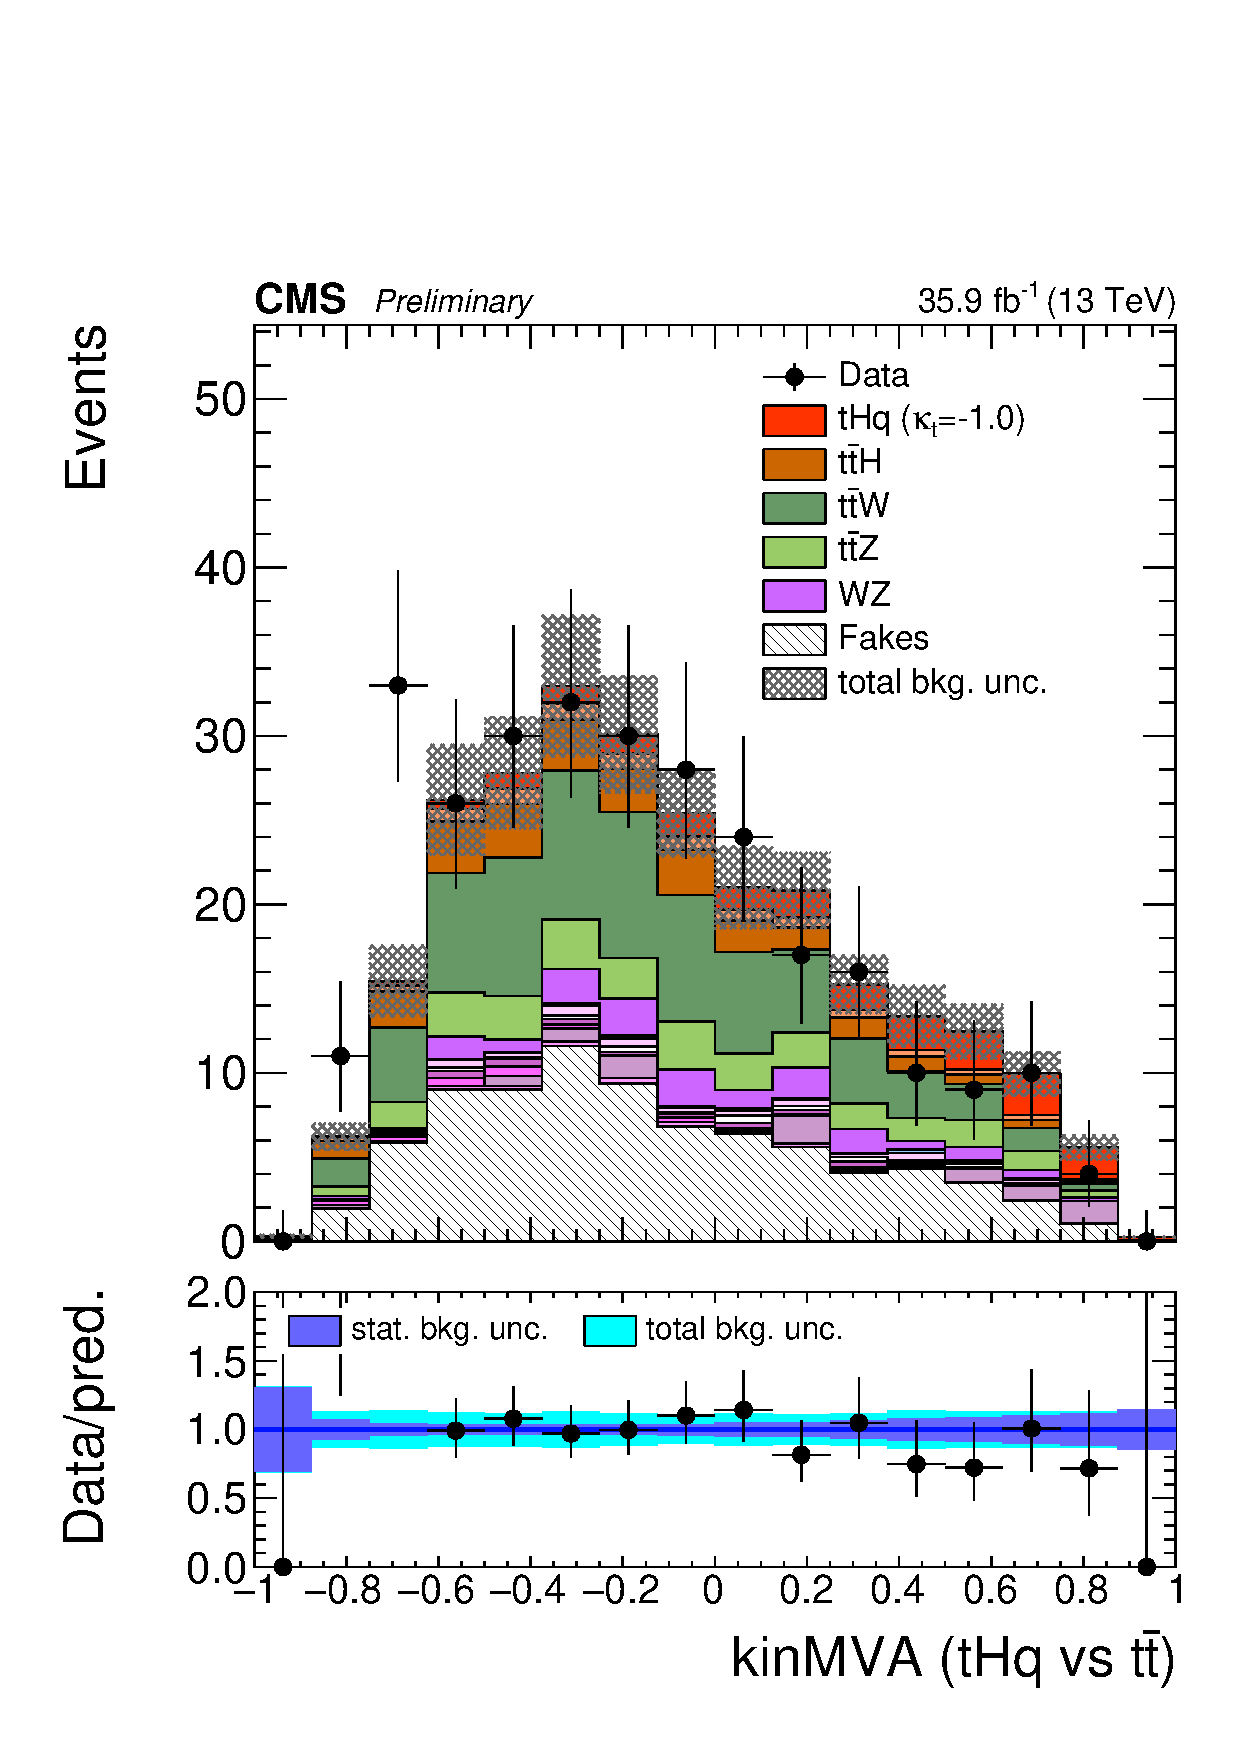
\includegraphics[width=0.32\textwidth]{figures/signalregion_2lss/mumu/thqMVA_tt_2lss_40.pdf}
 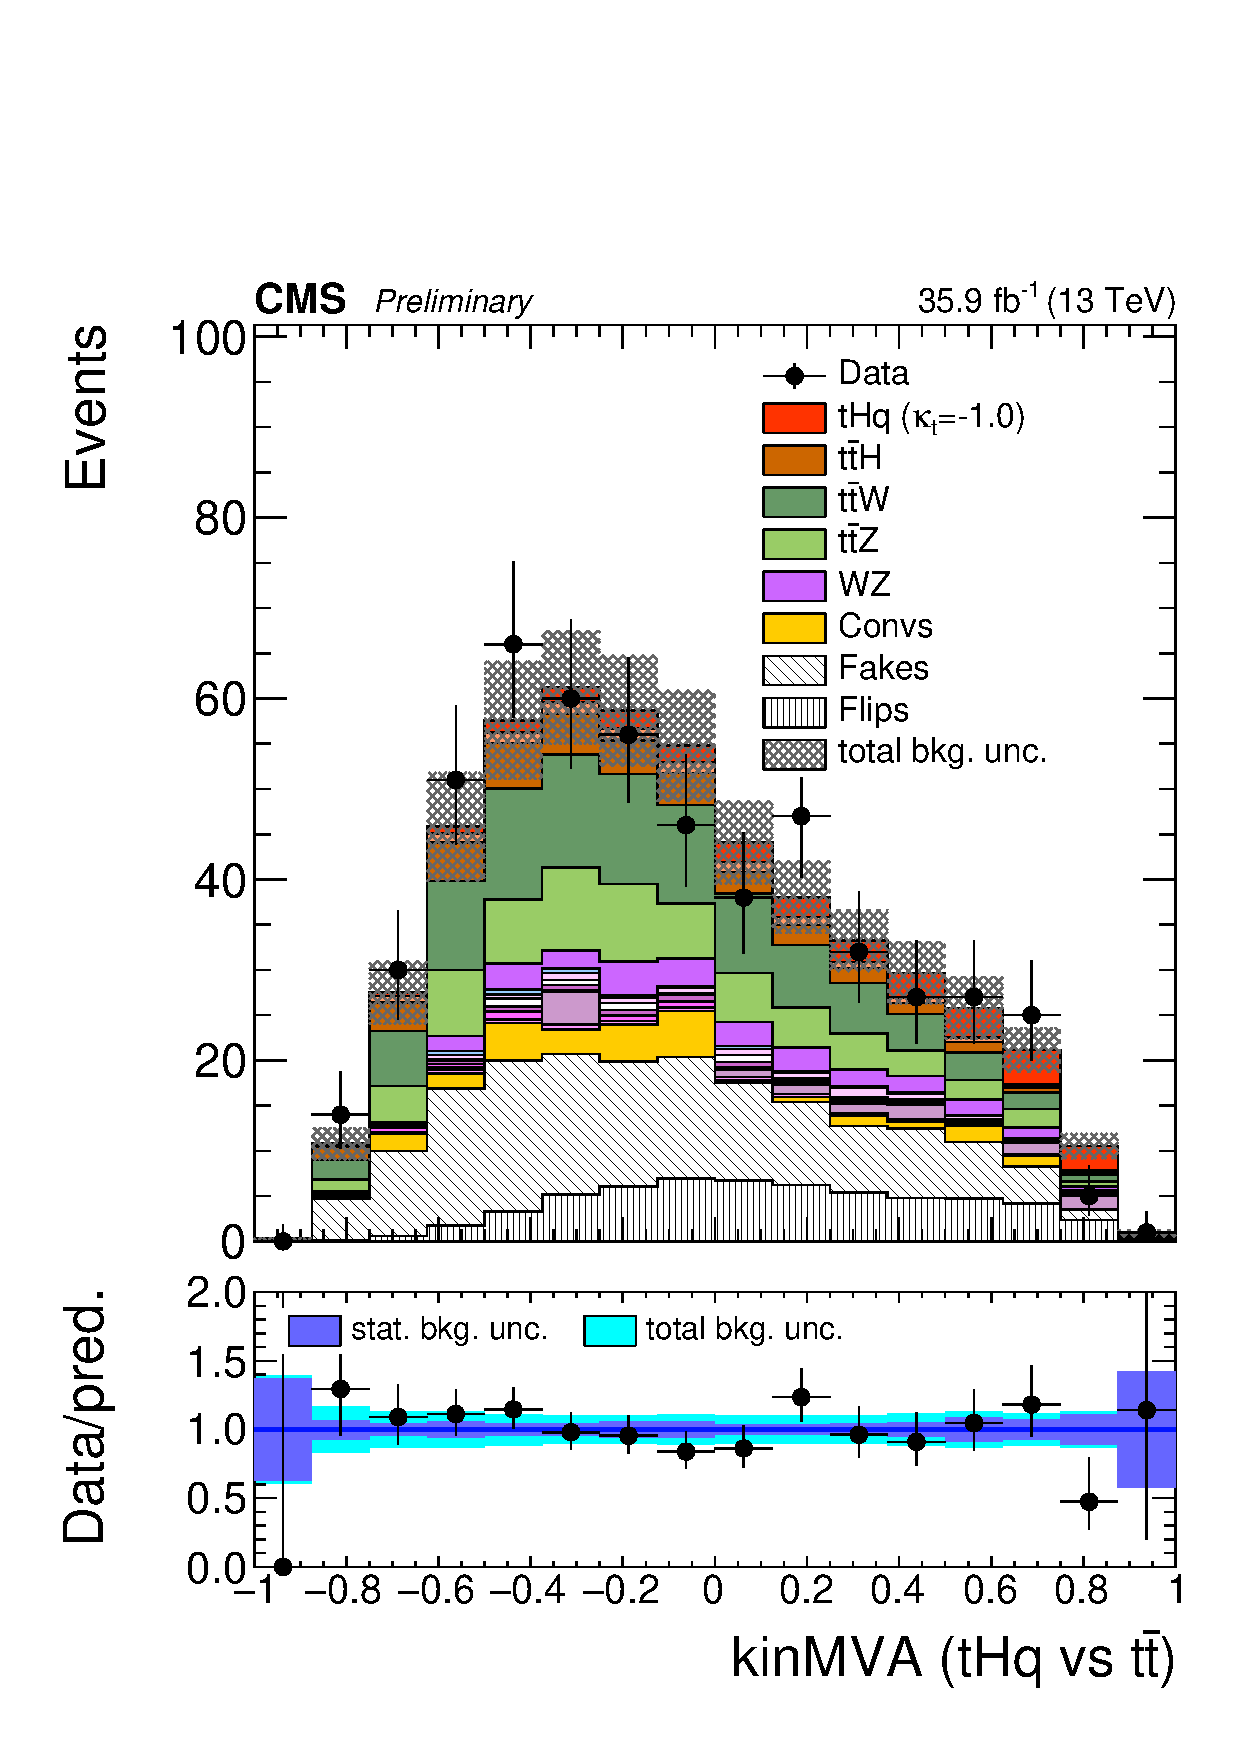
\includegraphics[width=0.32\textwidth]{figures/signalregion_2lss/emu/thqMVA_tt_2lss_40.pdf}
 % 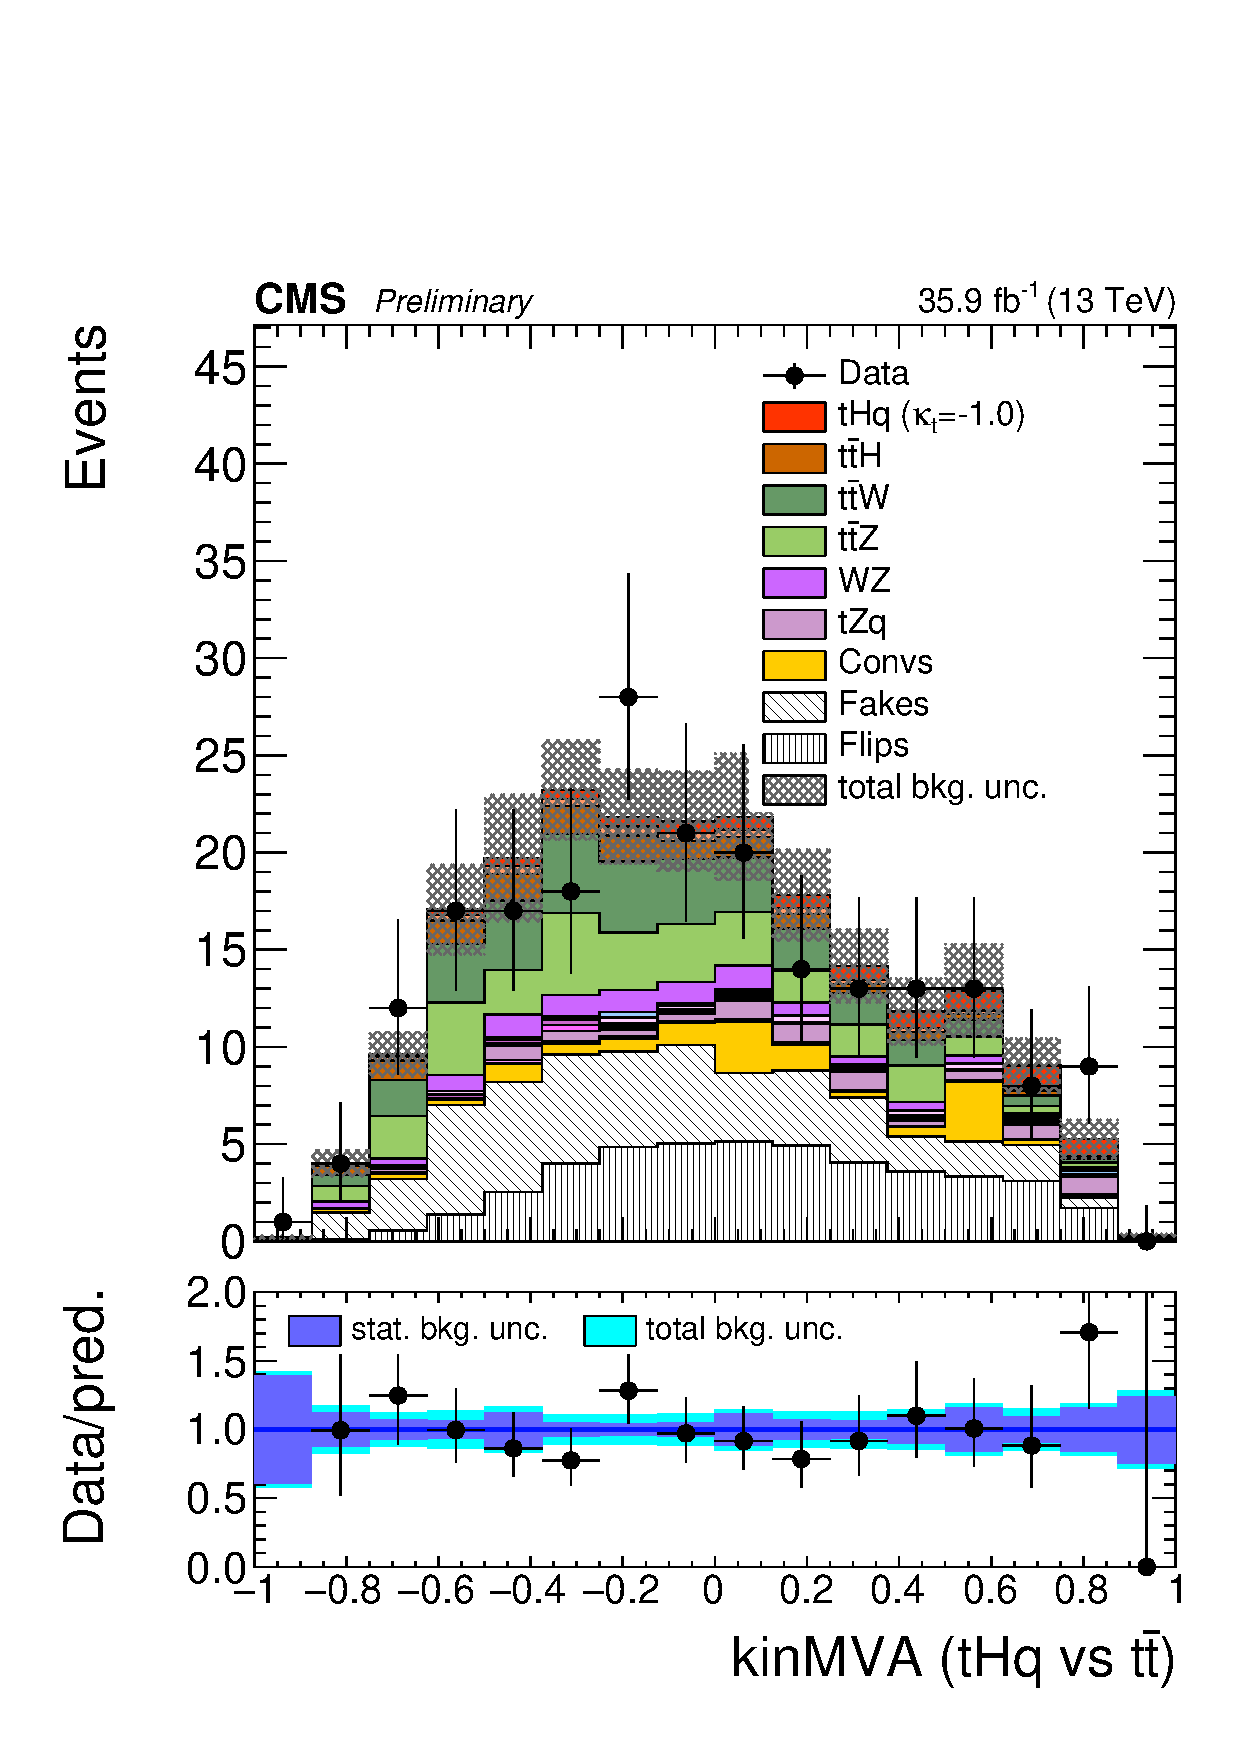
\includegraphics[width=0.24\textwidth]{figures/signalregion_2lss/ee/thqMVA_tt_2lss_40.pdf}
\
\caption{Distribution of individual BDT outputs for (from left to right) the three lepton channel, the \mumu\ channel, and the \emu\ channel, for training against \ttV\ (top row) and against \ttbar\ (bottom row).}
\label{fig:bdt_outputs}
\end{figure}

\begin{figure} [!h]
 \centering
 % 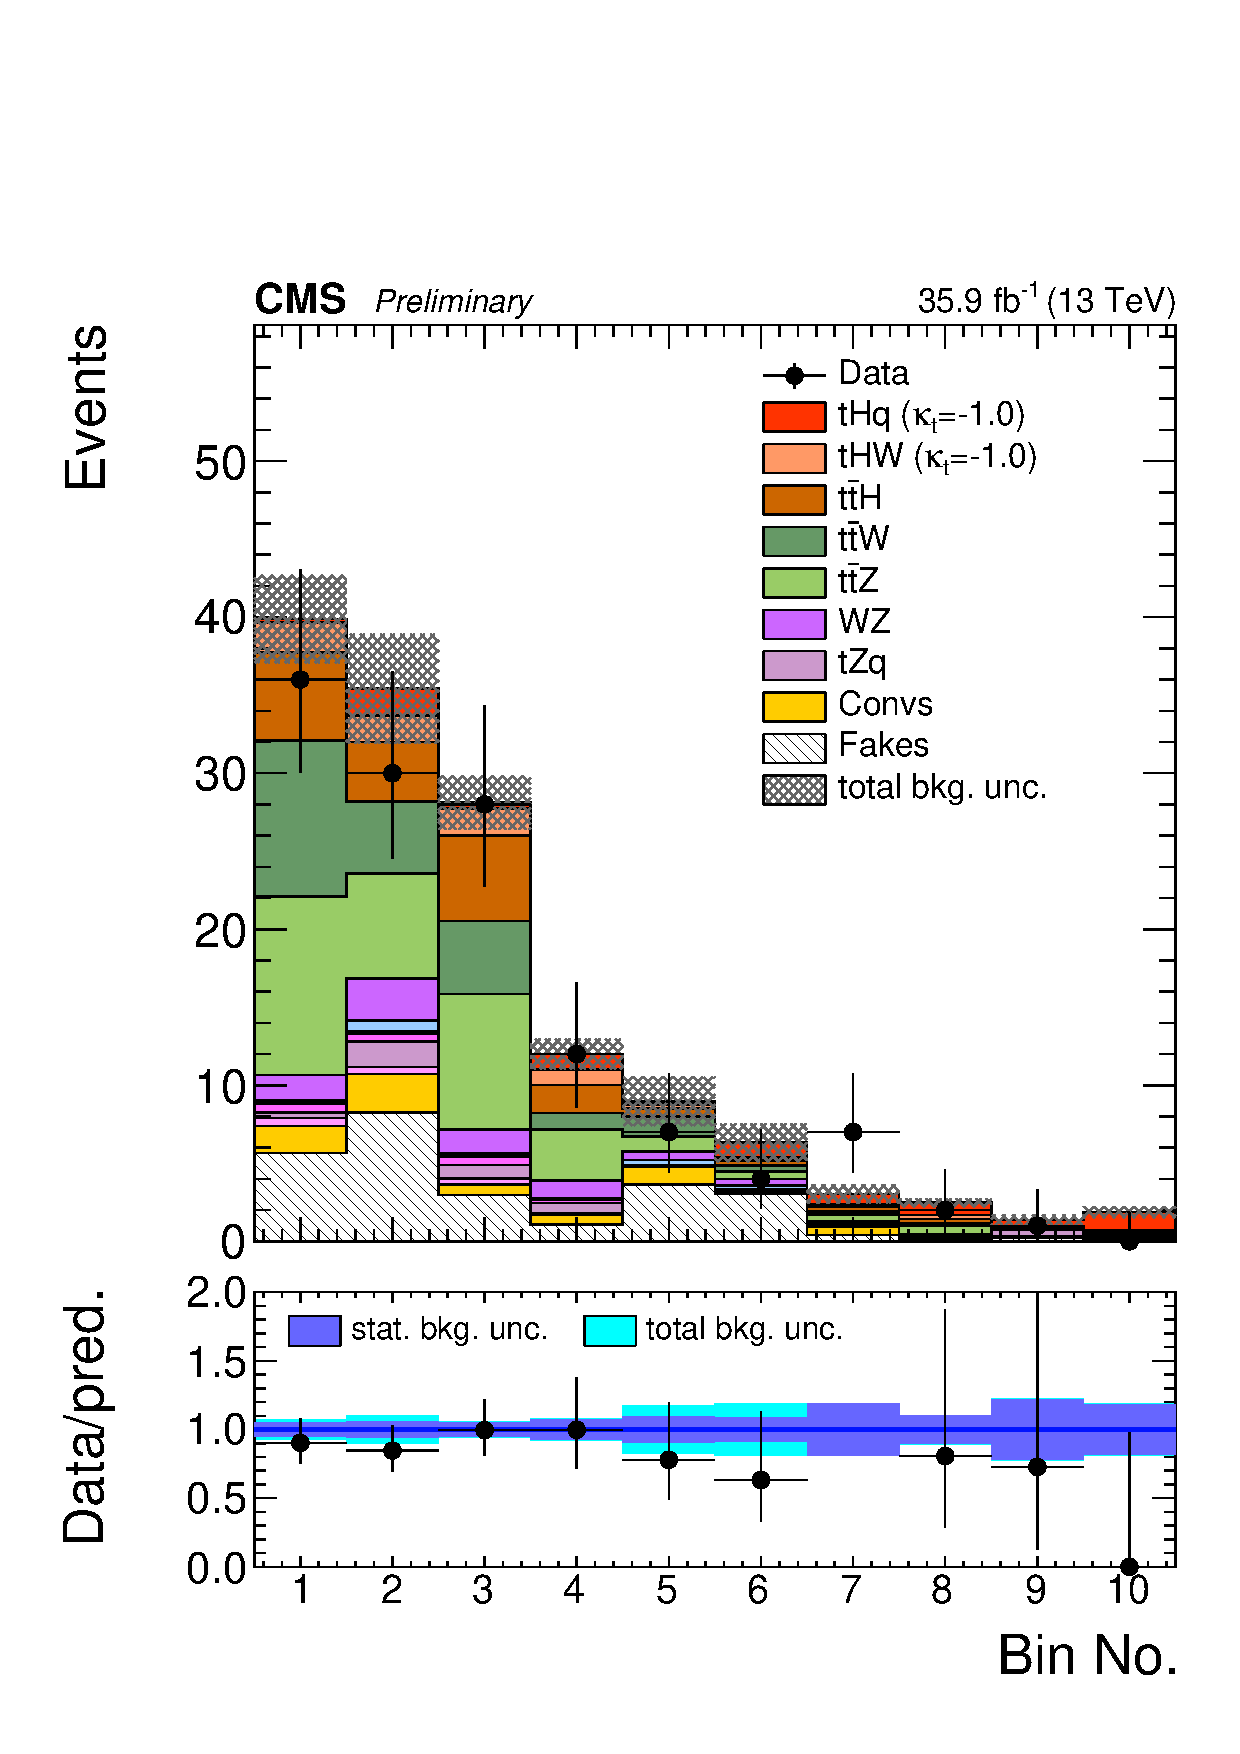
\includegraphics[width=0.24\textwidth]{figures/3lsignal/finalBins_40.pdf}
 % 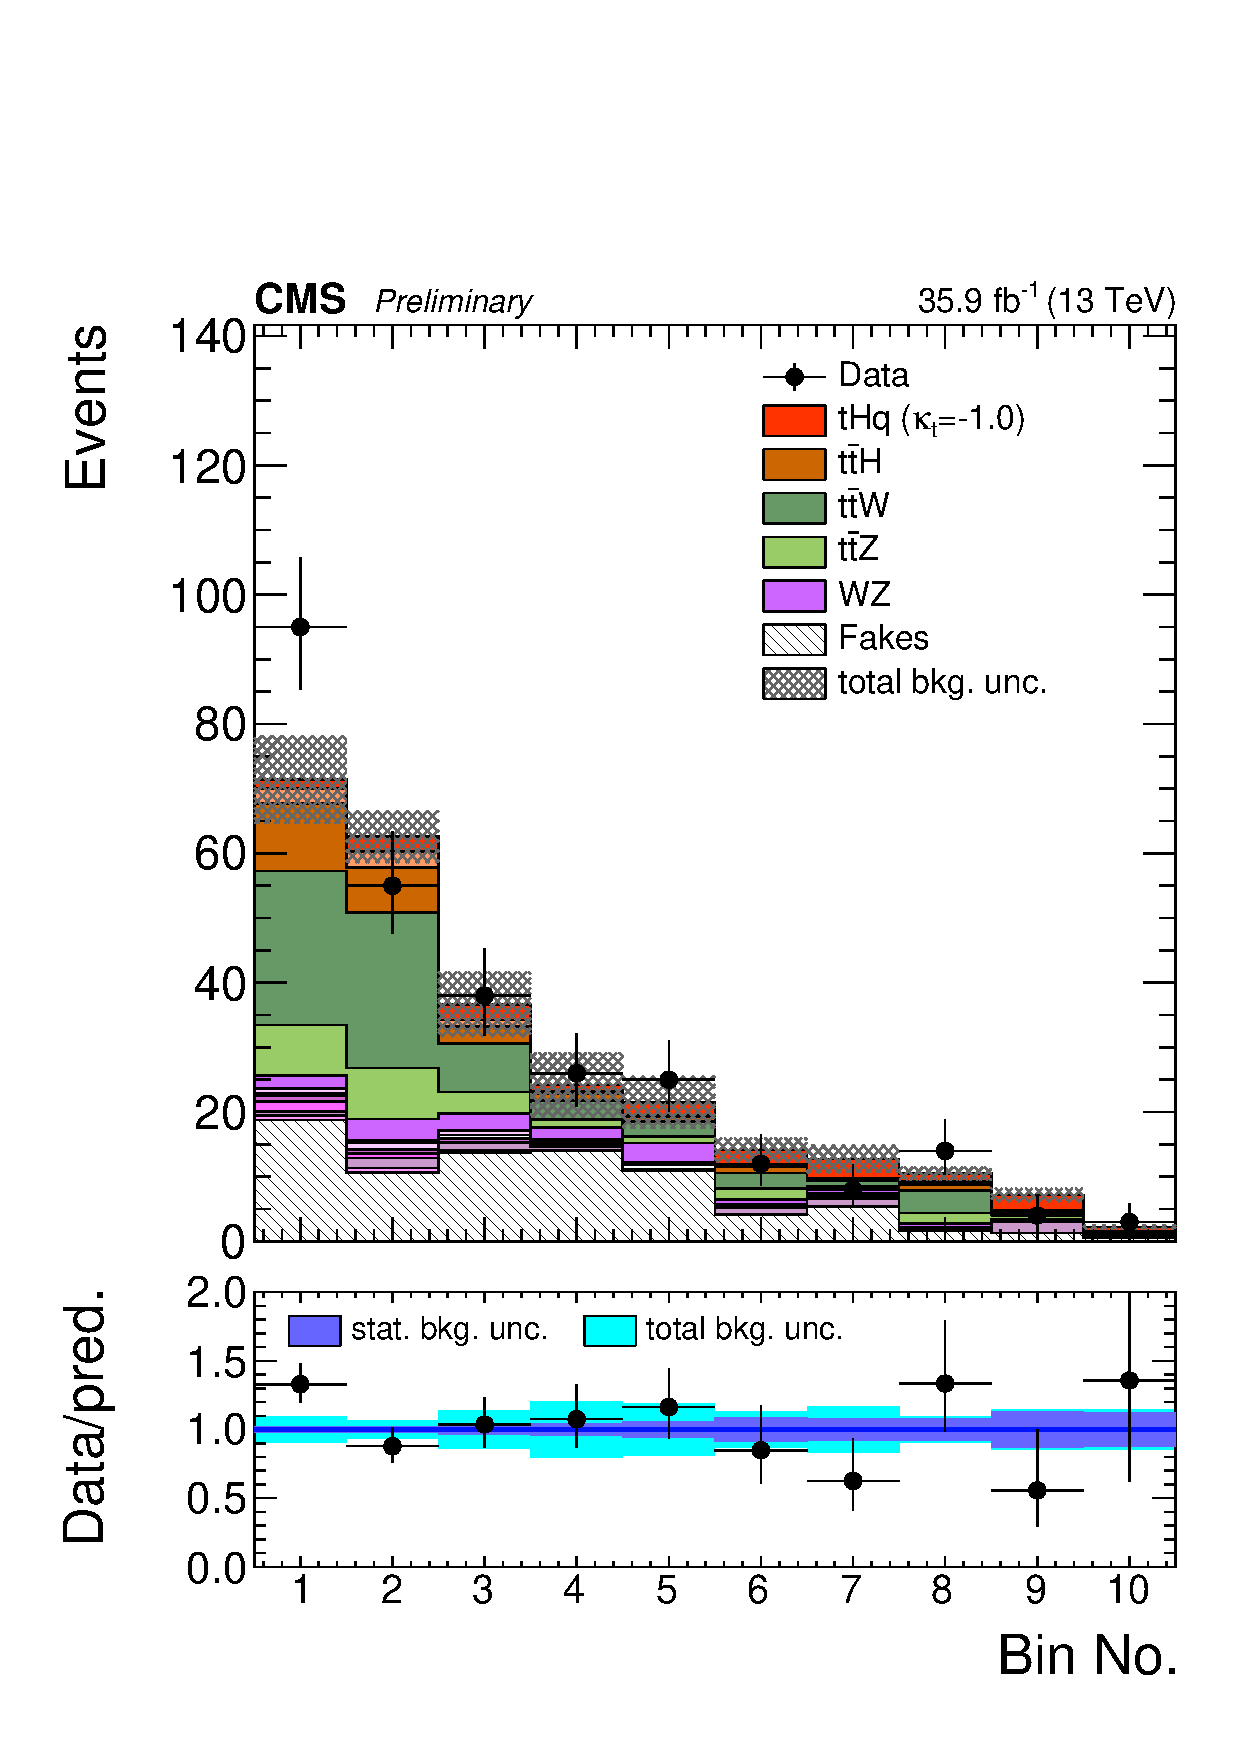
\includegraphics[width=0.24\textwidth]{figures/signalregion_2lss/mumu/finalBins_40.pdf}
 % 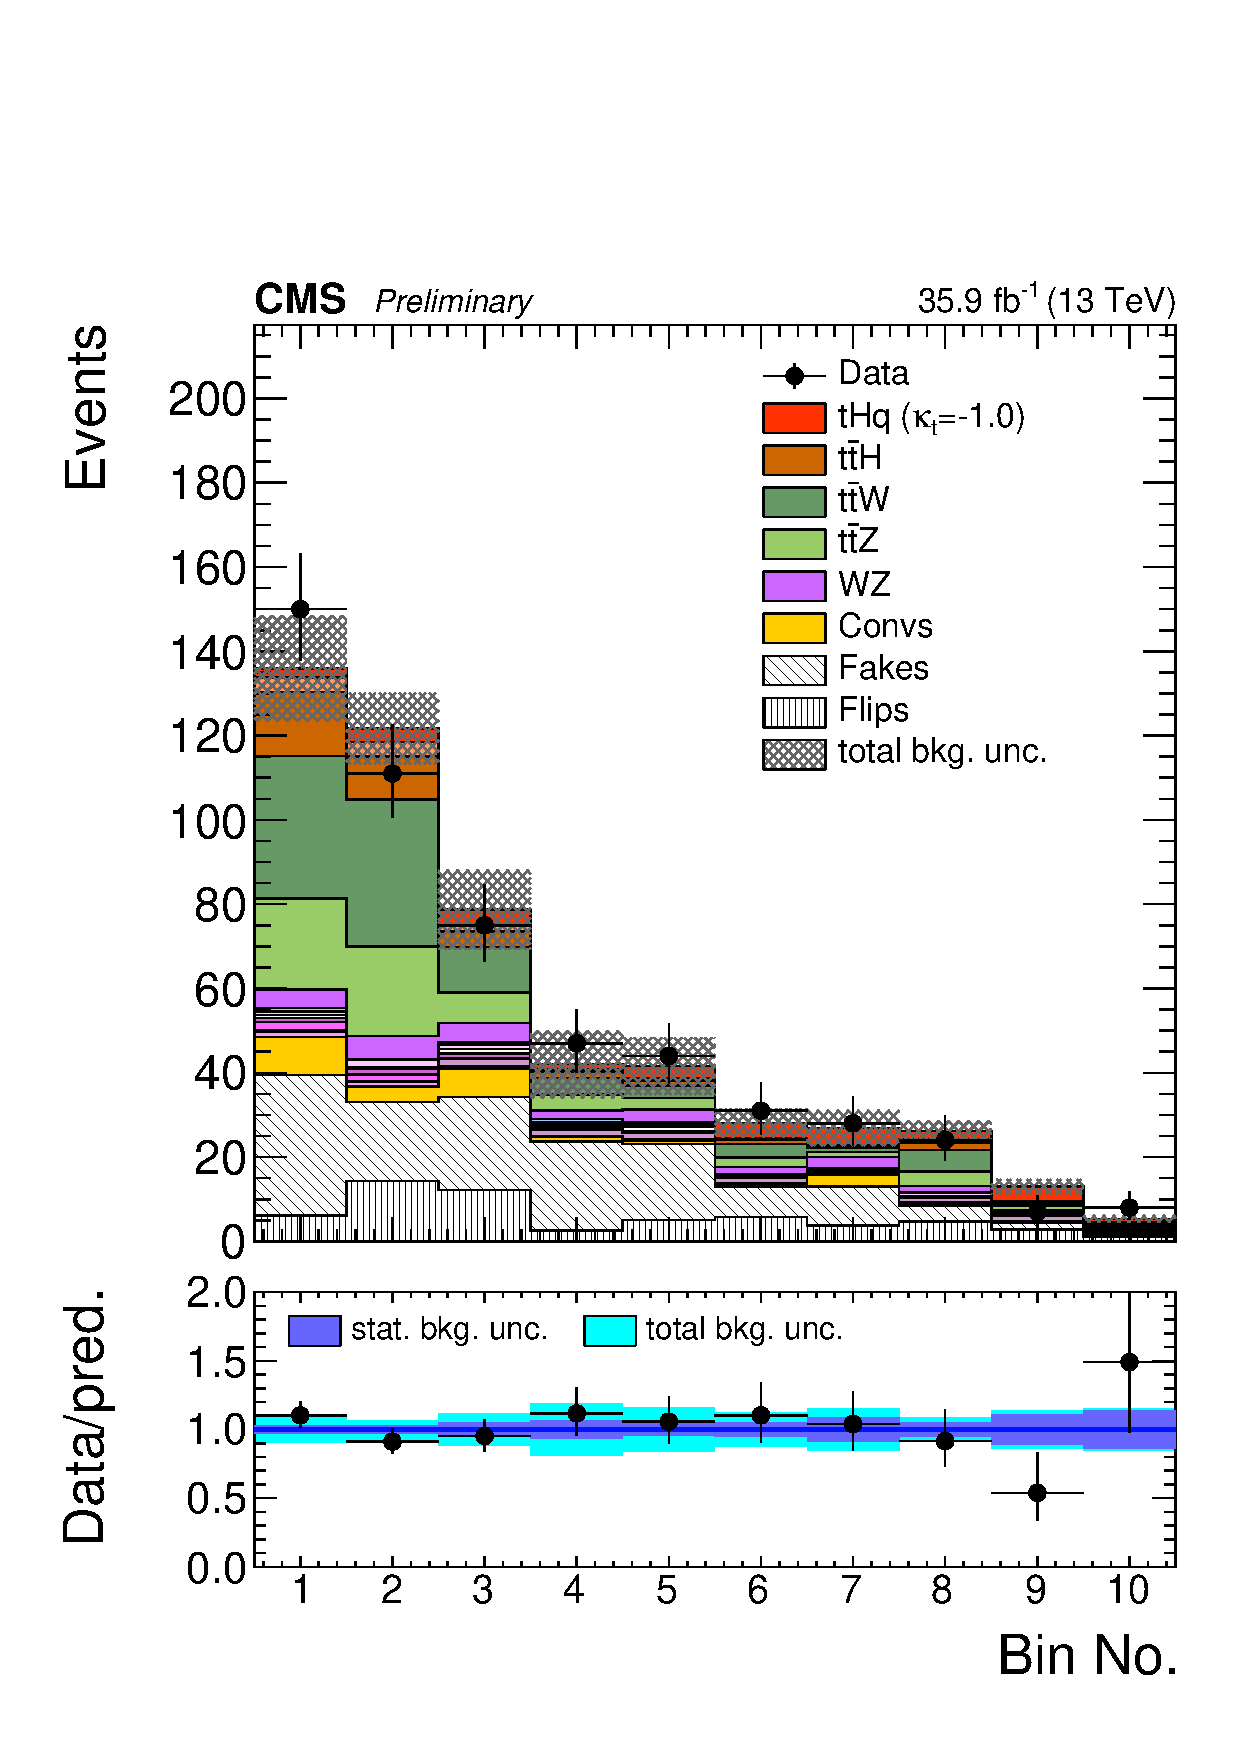
\includegraphics[width=0.24\textwidth]{figures/signalregion_2lss/emu/finalBins_40.pdf}
 % 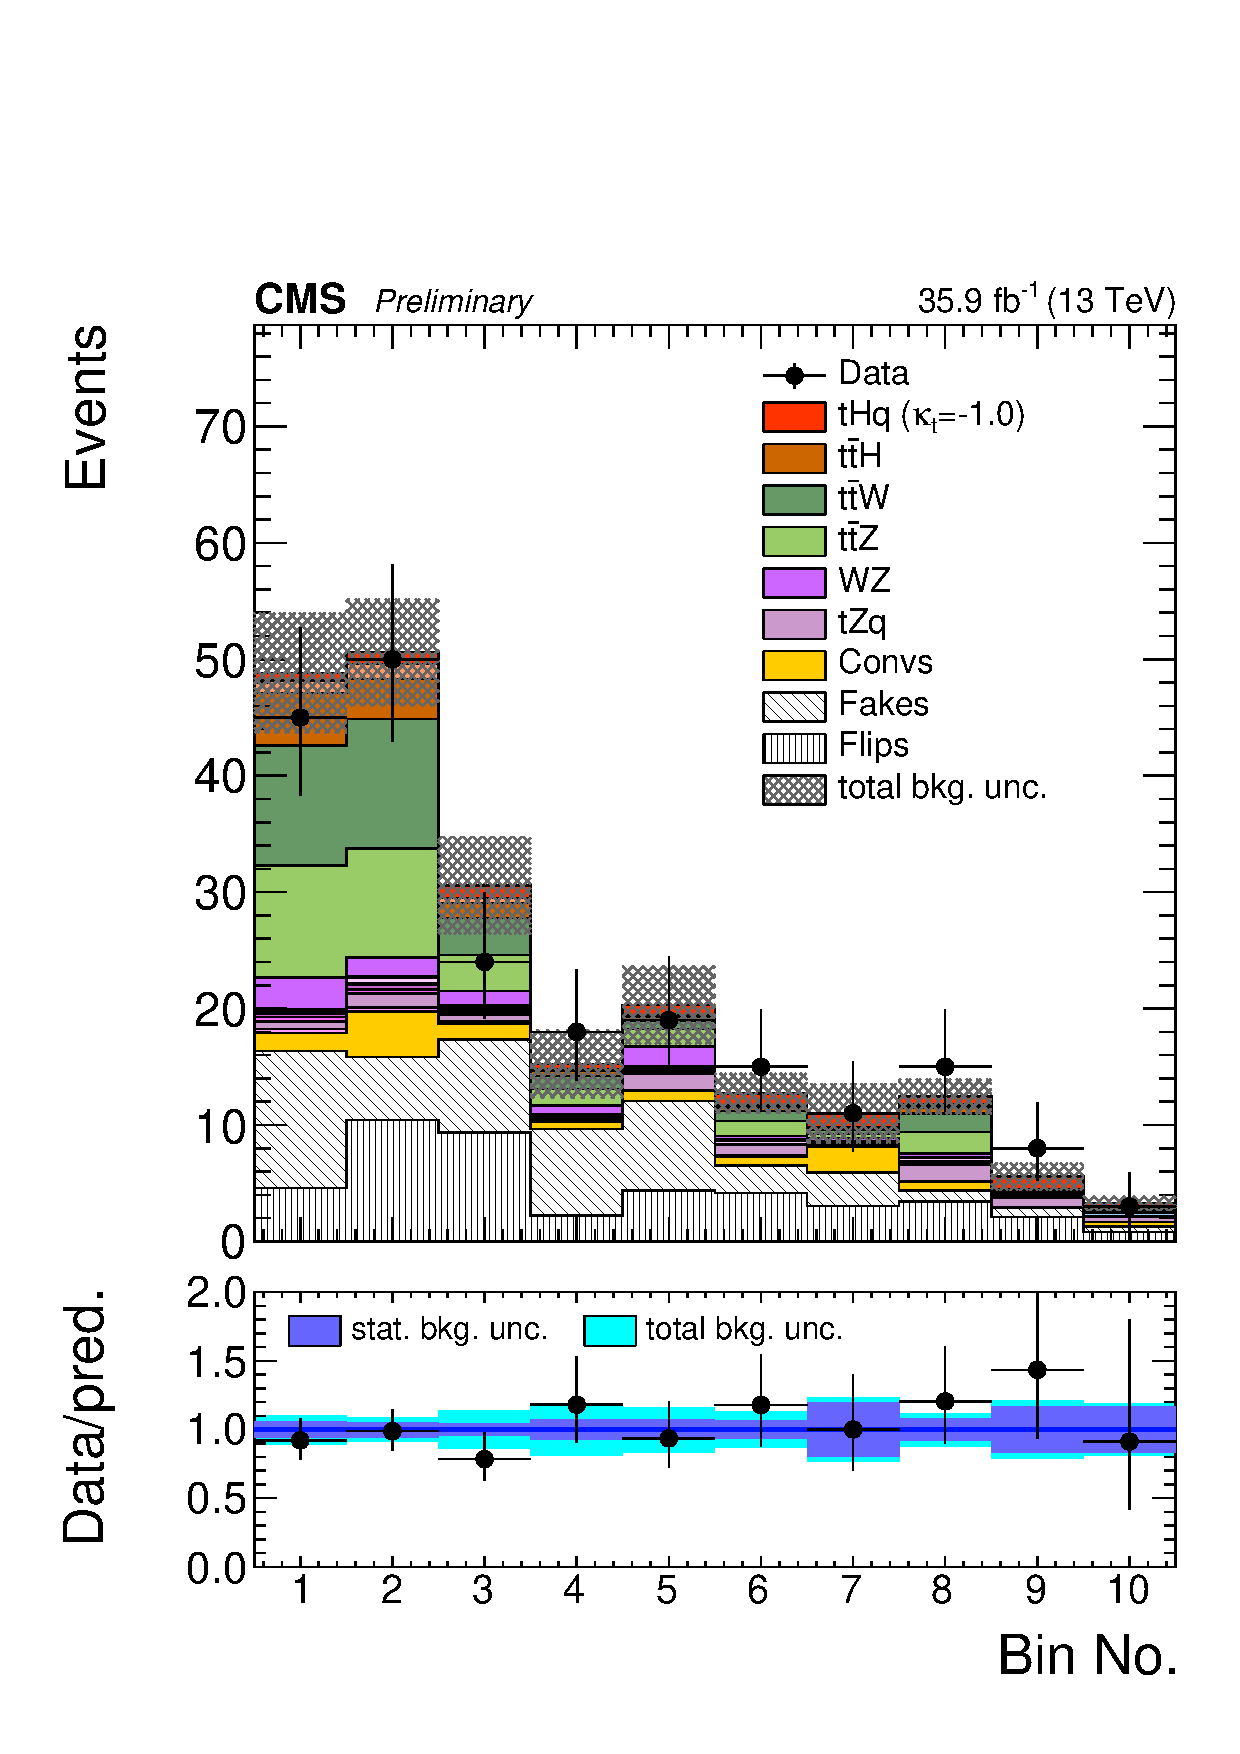
\includegraphics[width=0.24\textwidth]{figures/signalregion_2lss/ee/finalBins_40.pdf} \\
 % 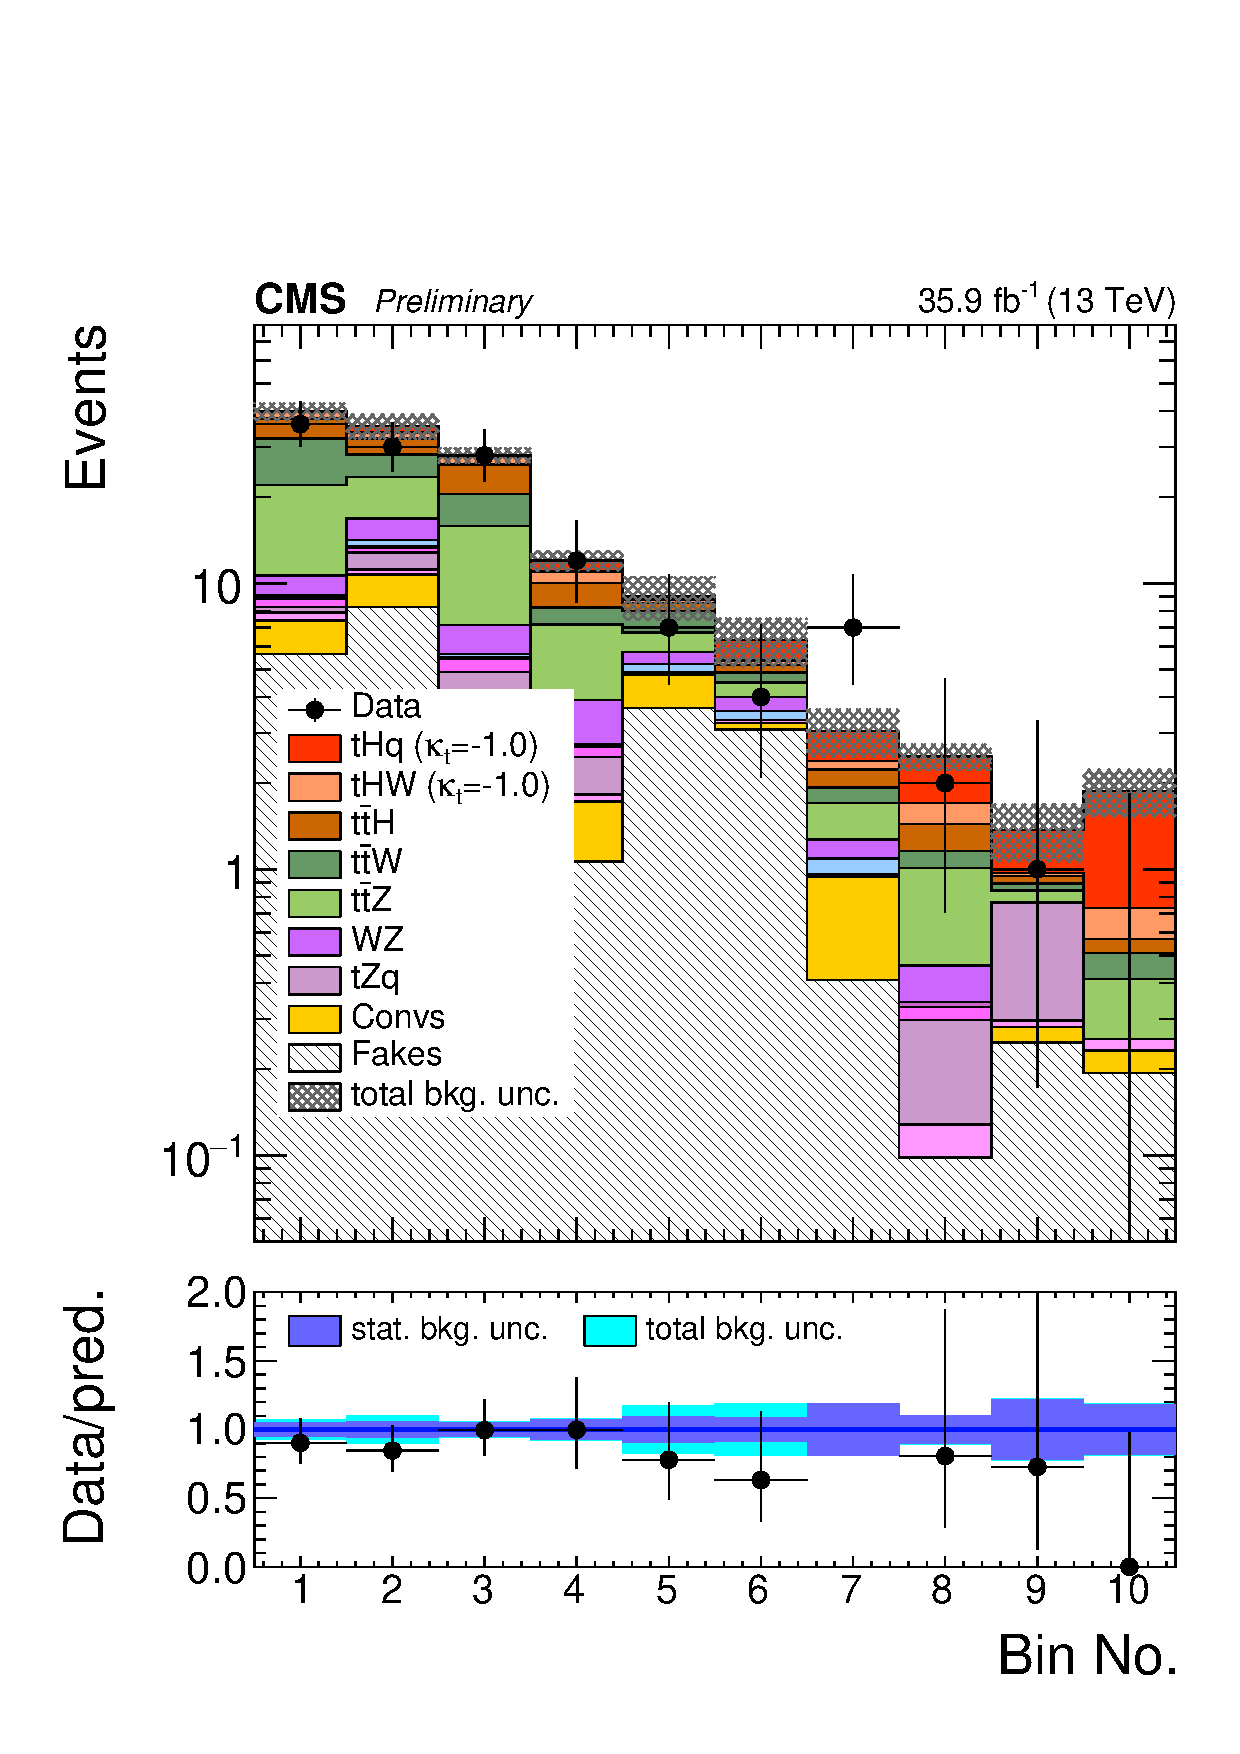
\includegraphics[width=0.24\textwidth]{figures/3lsignal/finalBins_log_40.pdf}
 % 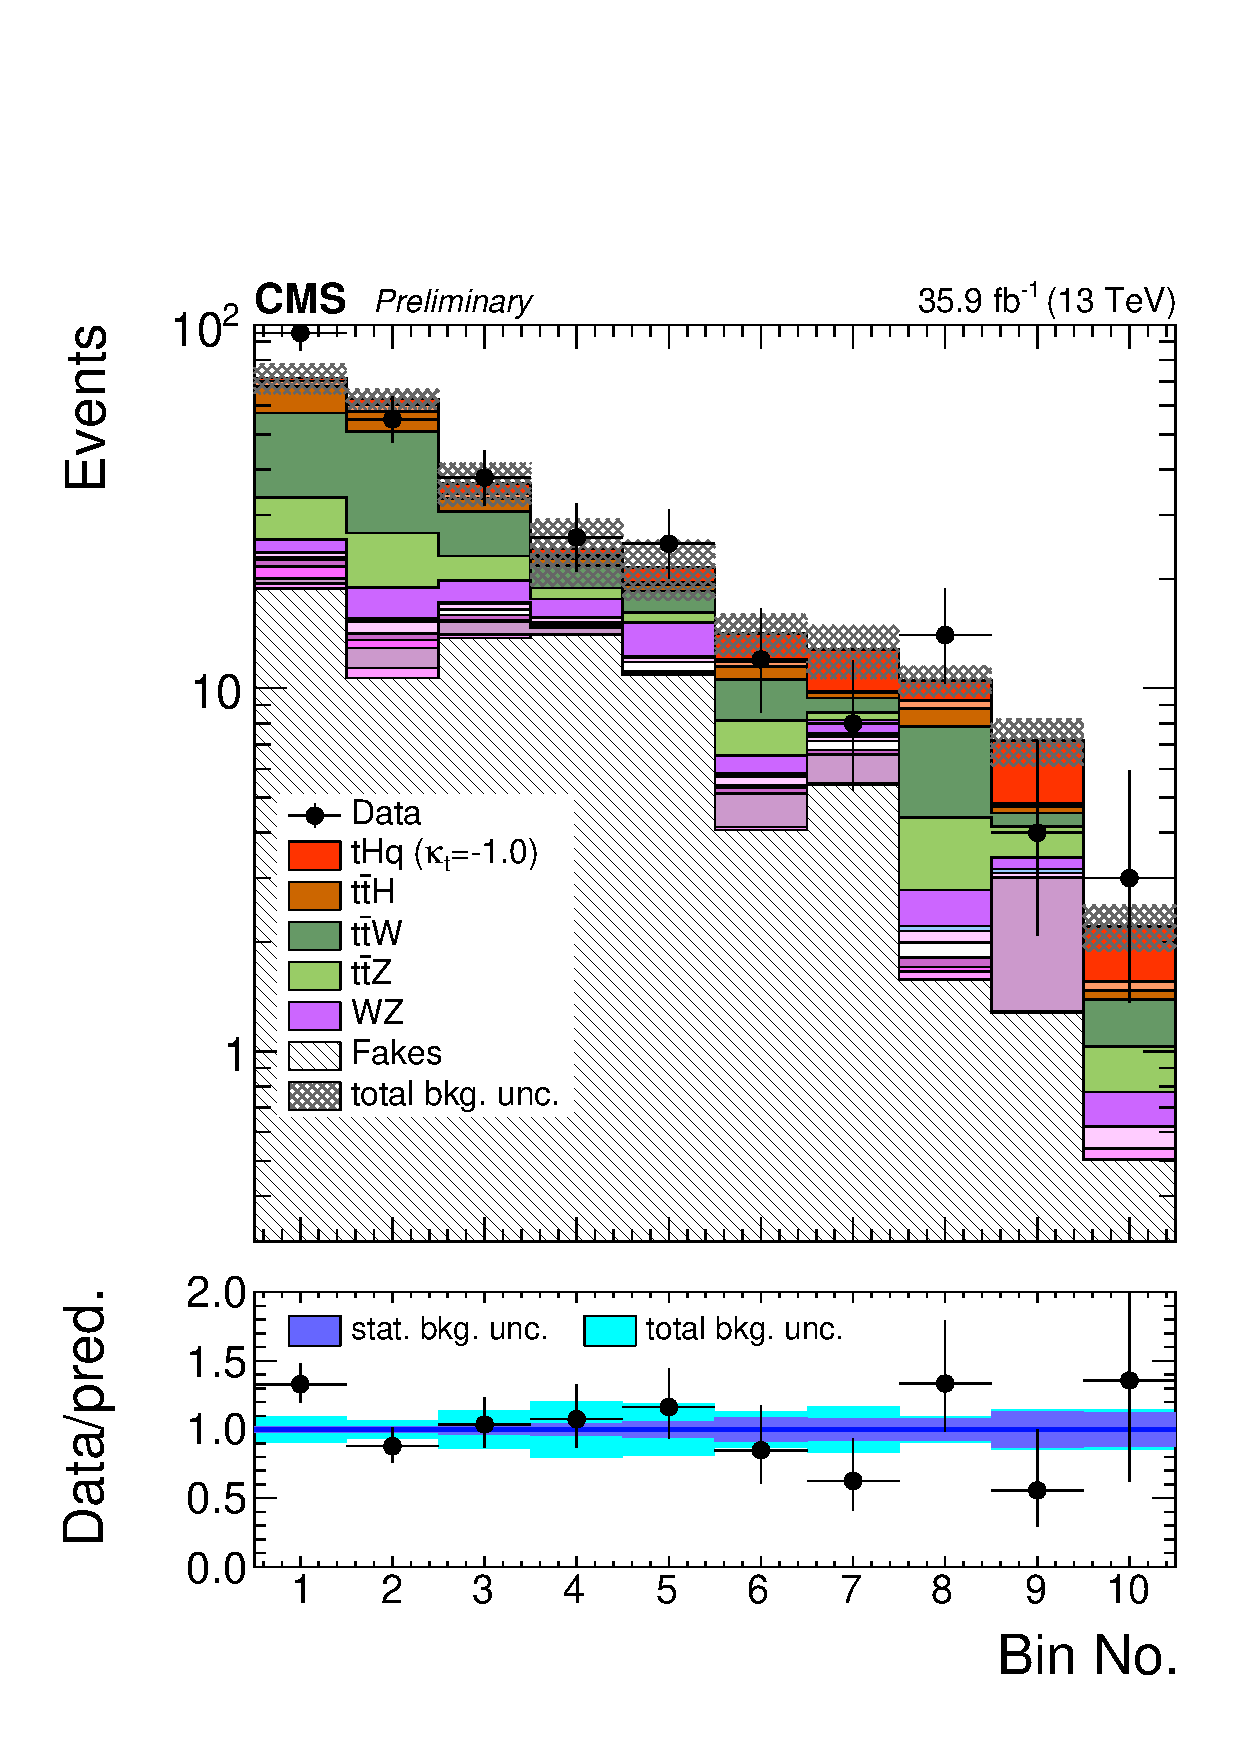
\includegraphics[width=0.24\textwidth]{figures/signalregion_2lss/mumu/finalBins_log_mm_40.pdf}
 % 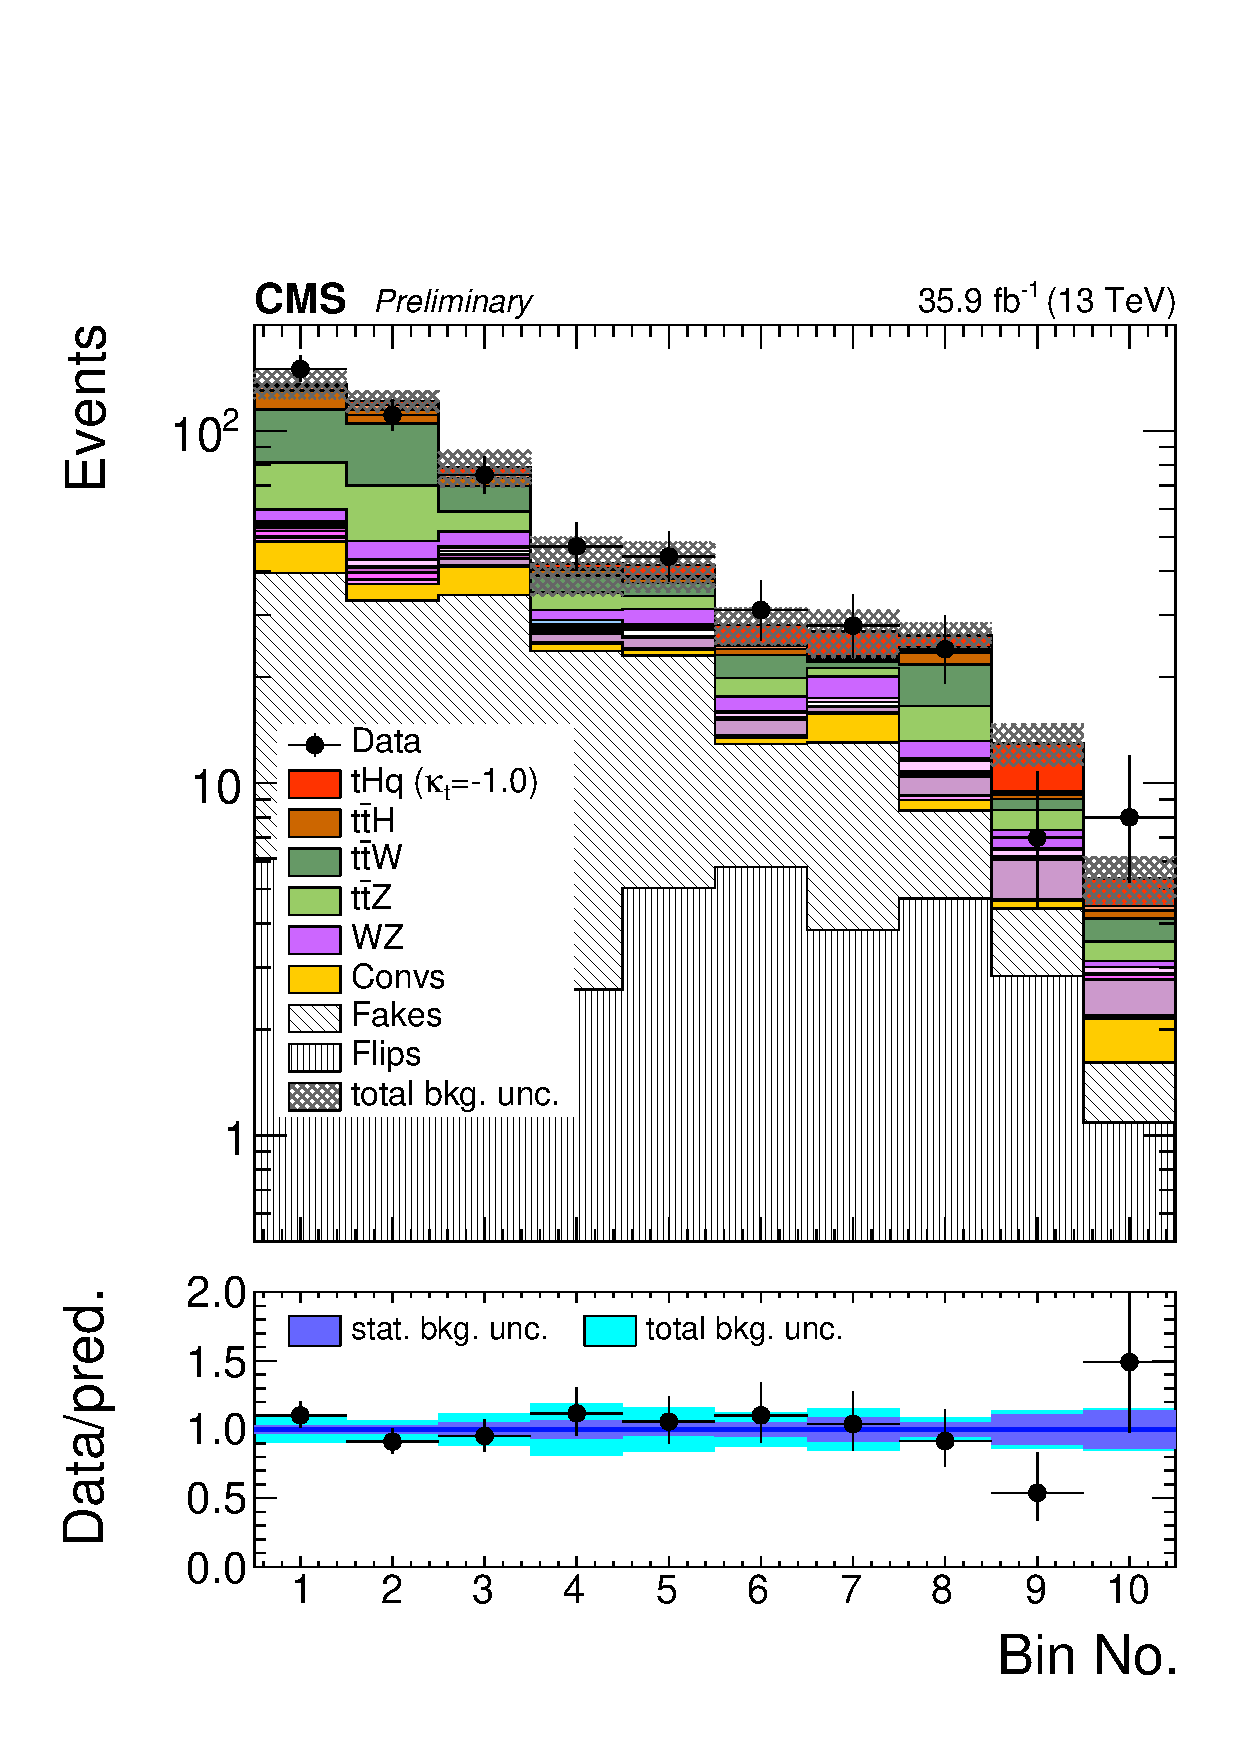
\includegraphics[width=0.24\textwidth]{figures/signalregion_2lss/emu/finalBins_log_em_40.pdf}
 % 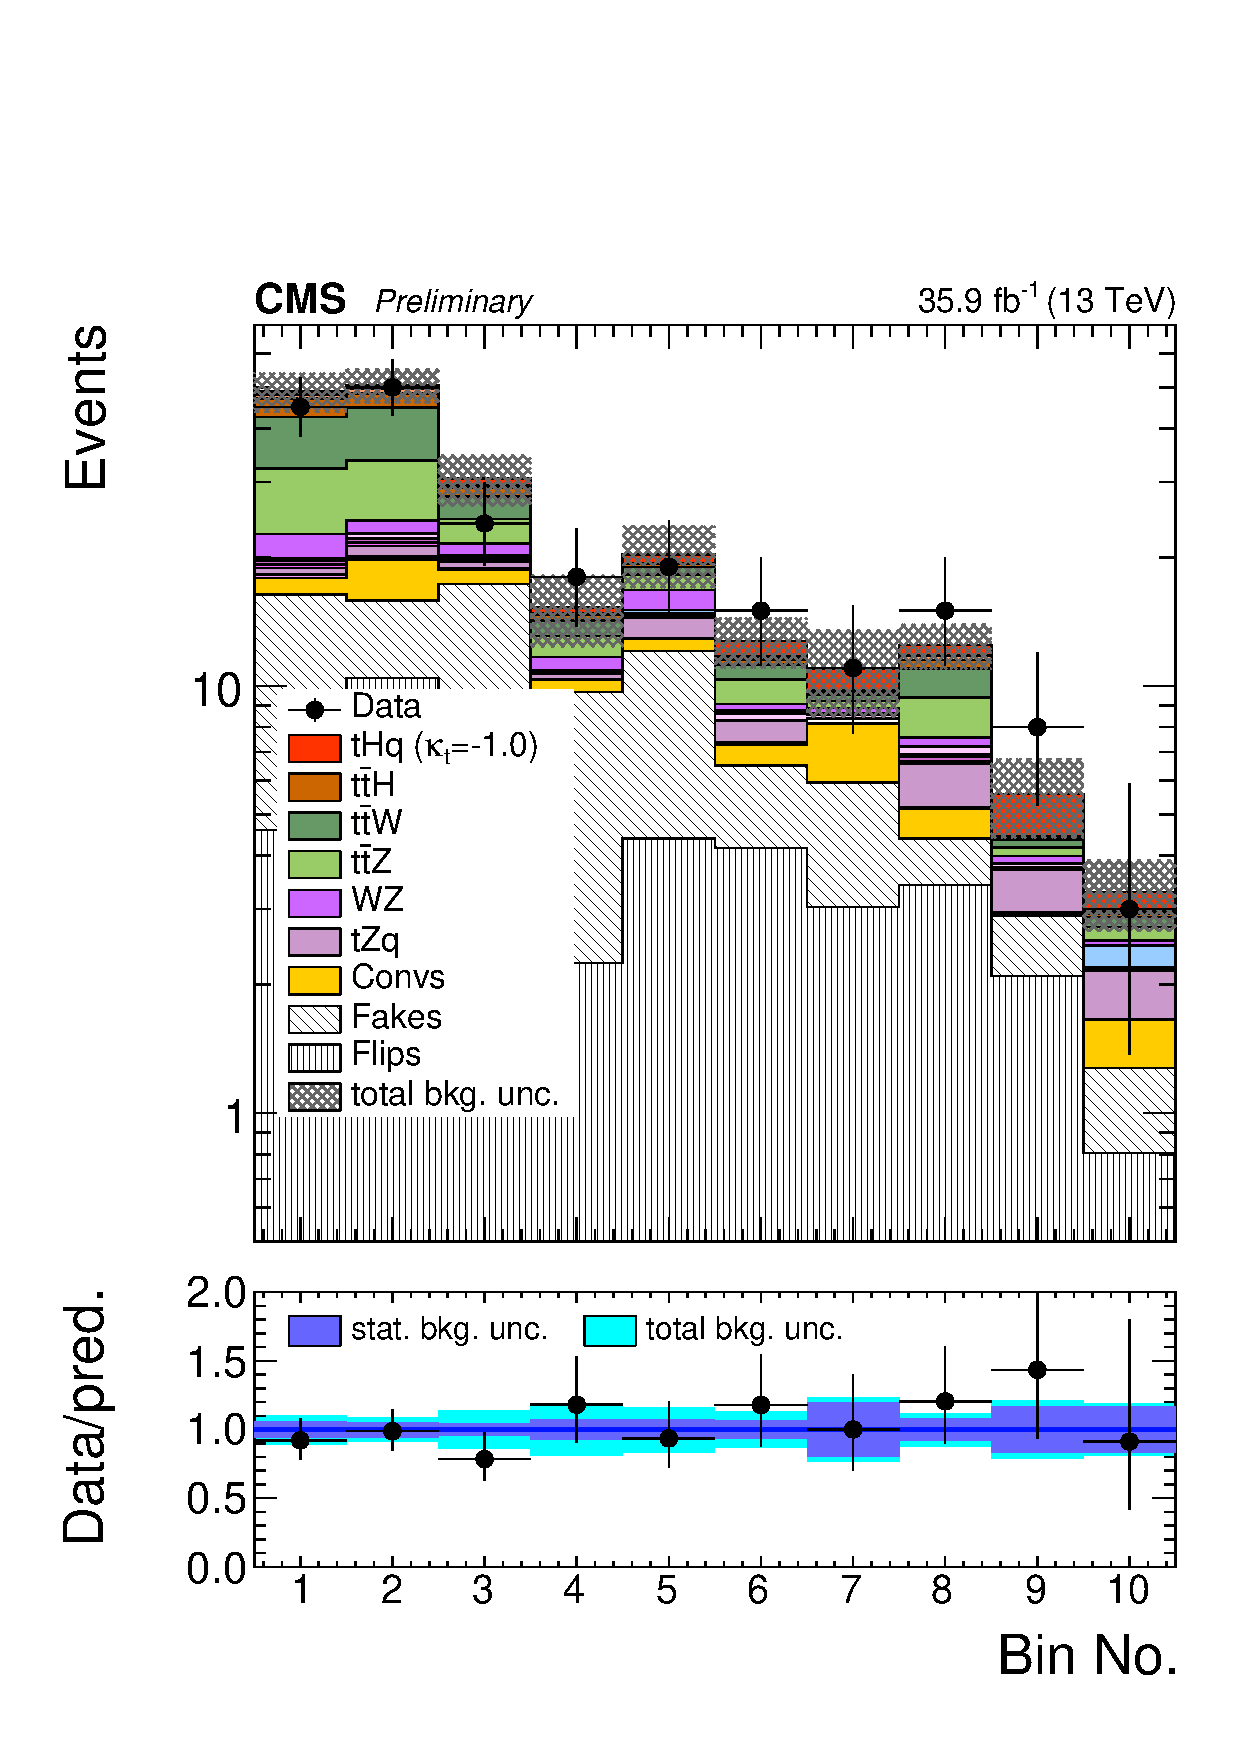
\includegraphics[width=0.24\textwidth]{figures/signalregion_2lss/ee/finalBins_log_ee_40.pdf}
 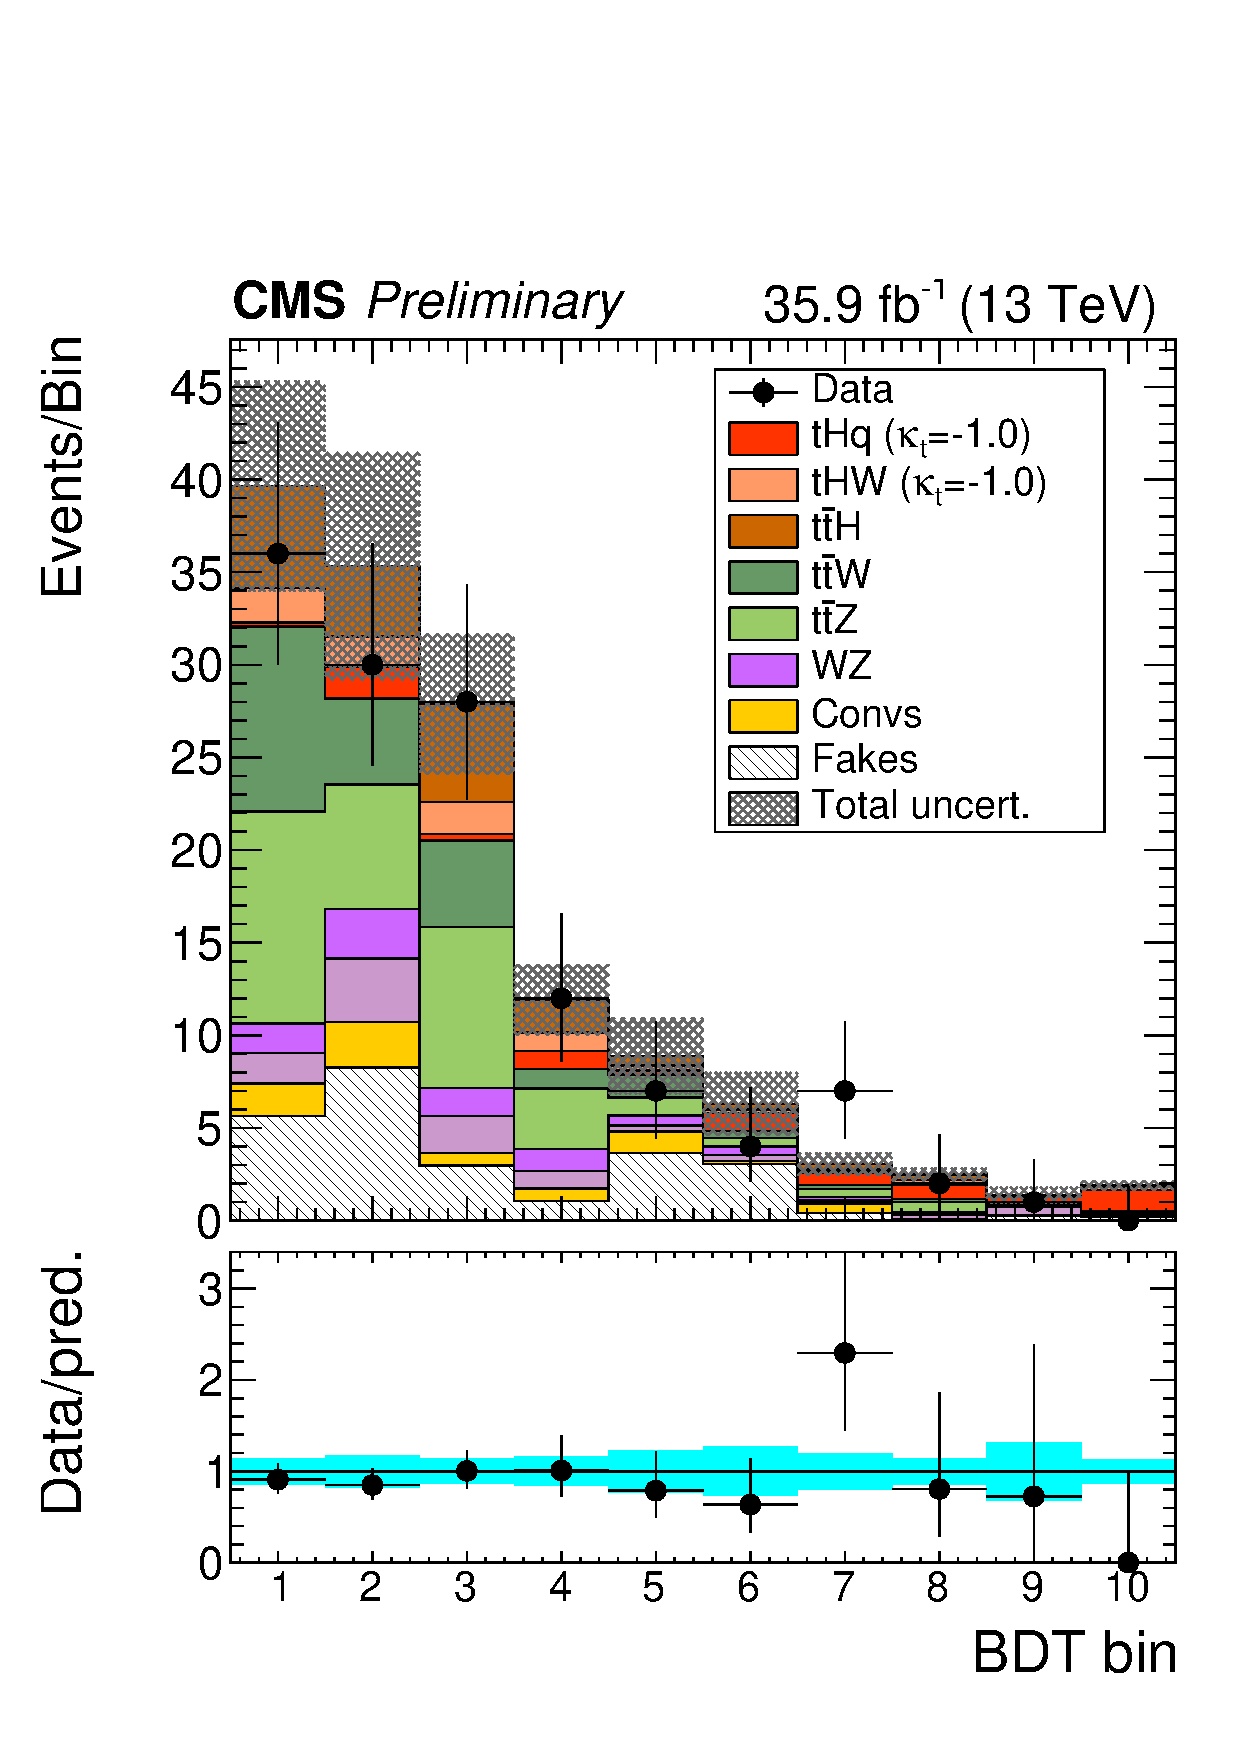
\includegraphics[width=0.32\textwidth]{figures/postfit/tHq_3l_13TeV_prefit.pdf}
 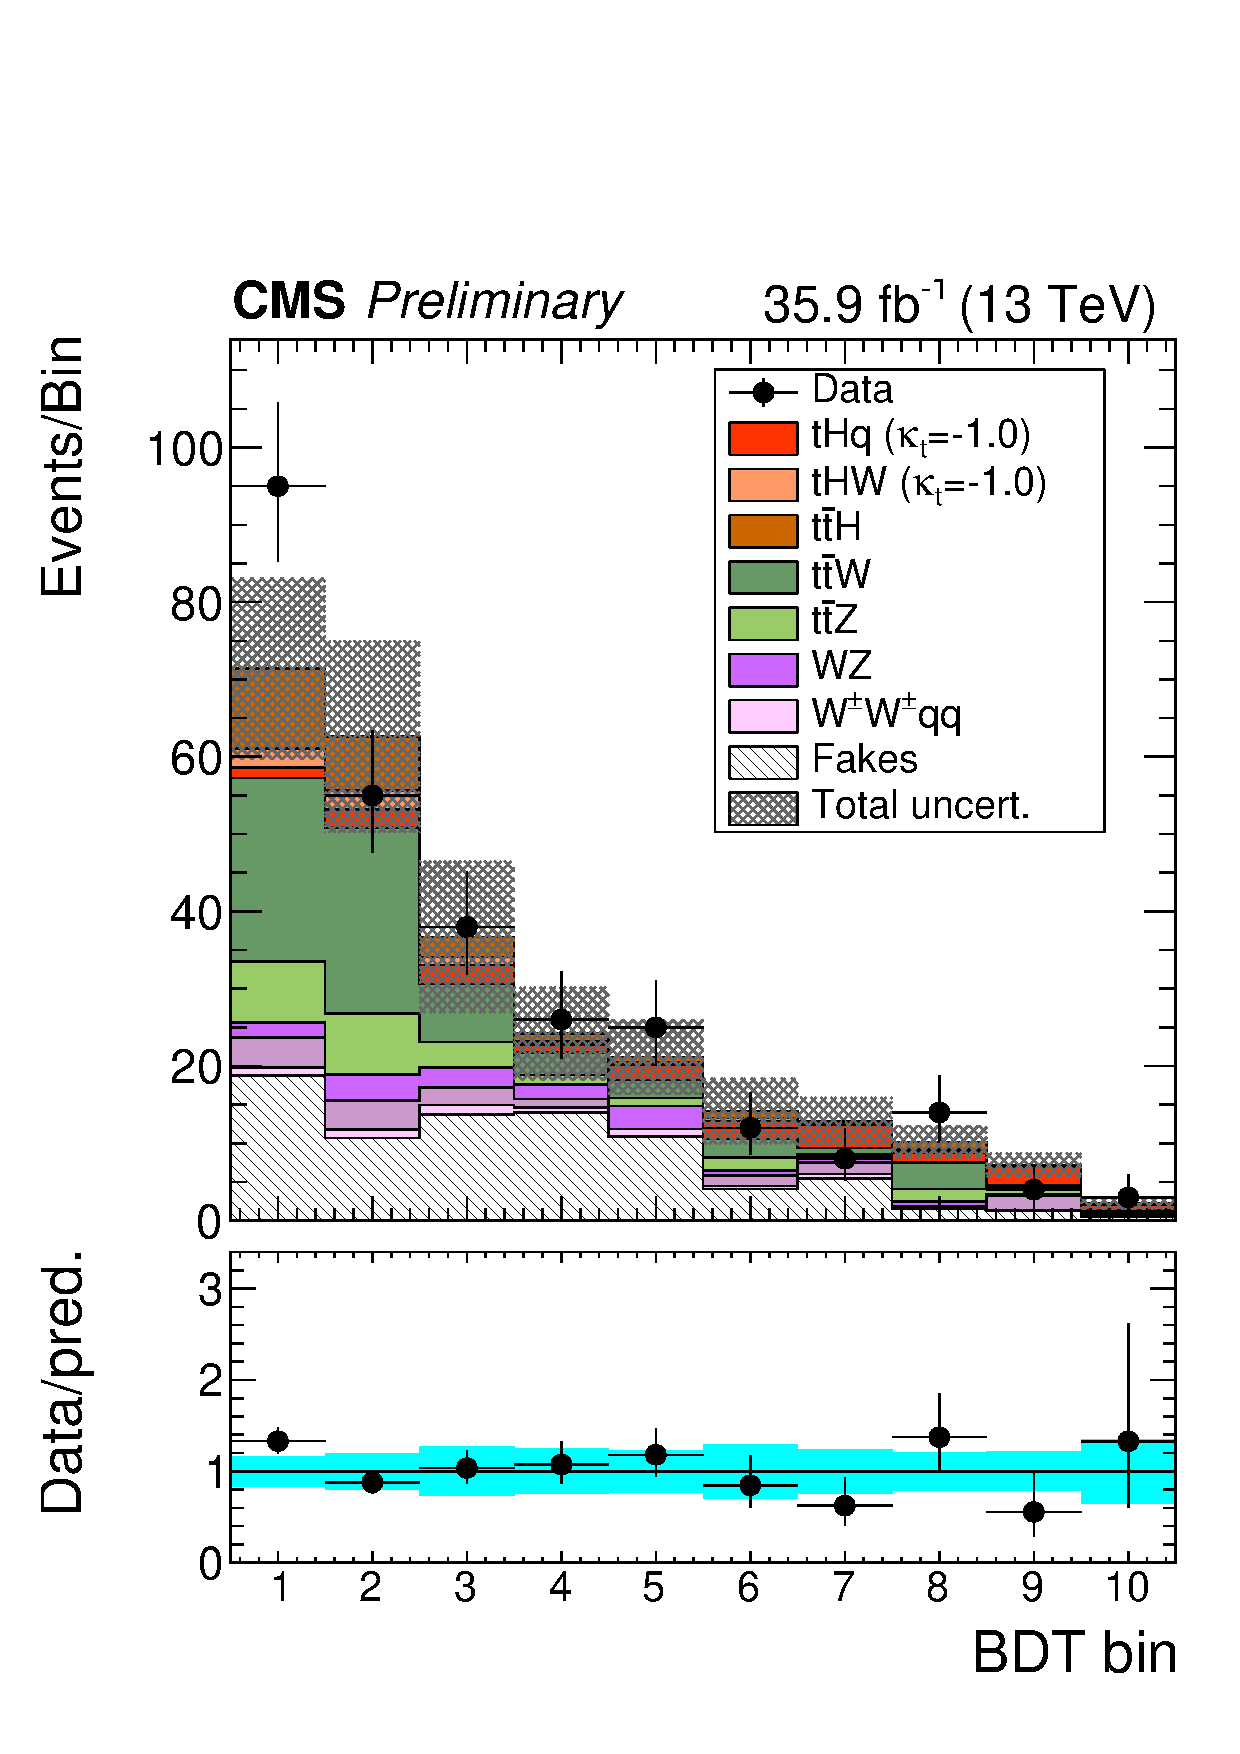
\includegraphics[width=0.32\textwidth]{figures/postfit/tHq_2lss_mm_13TeV_prefit.pdf}
 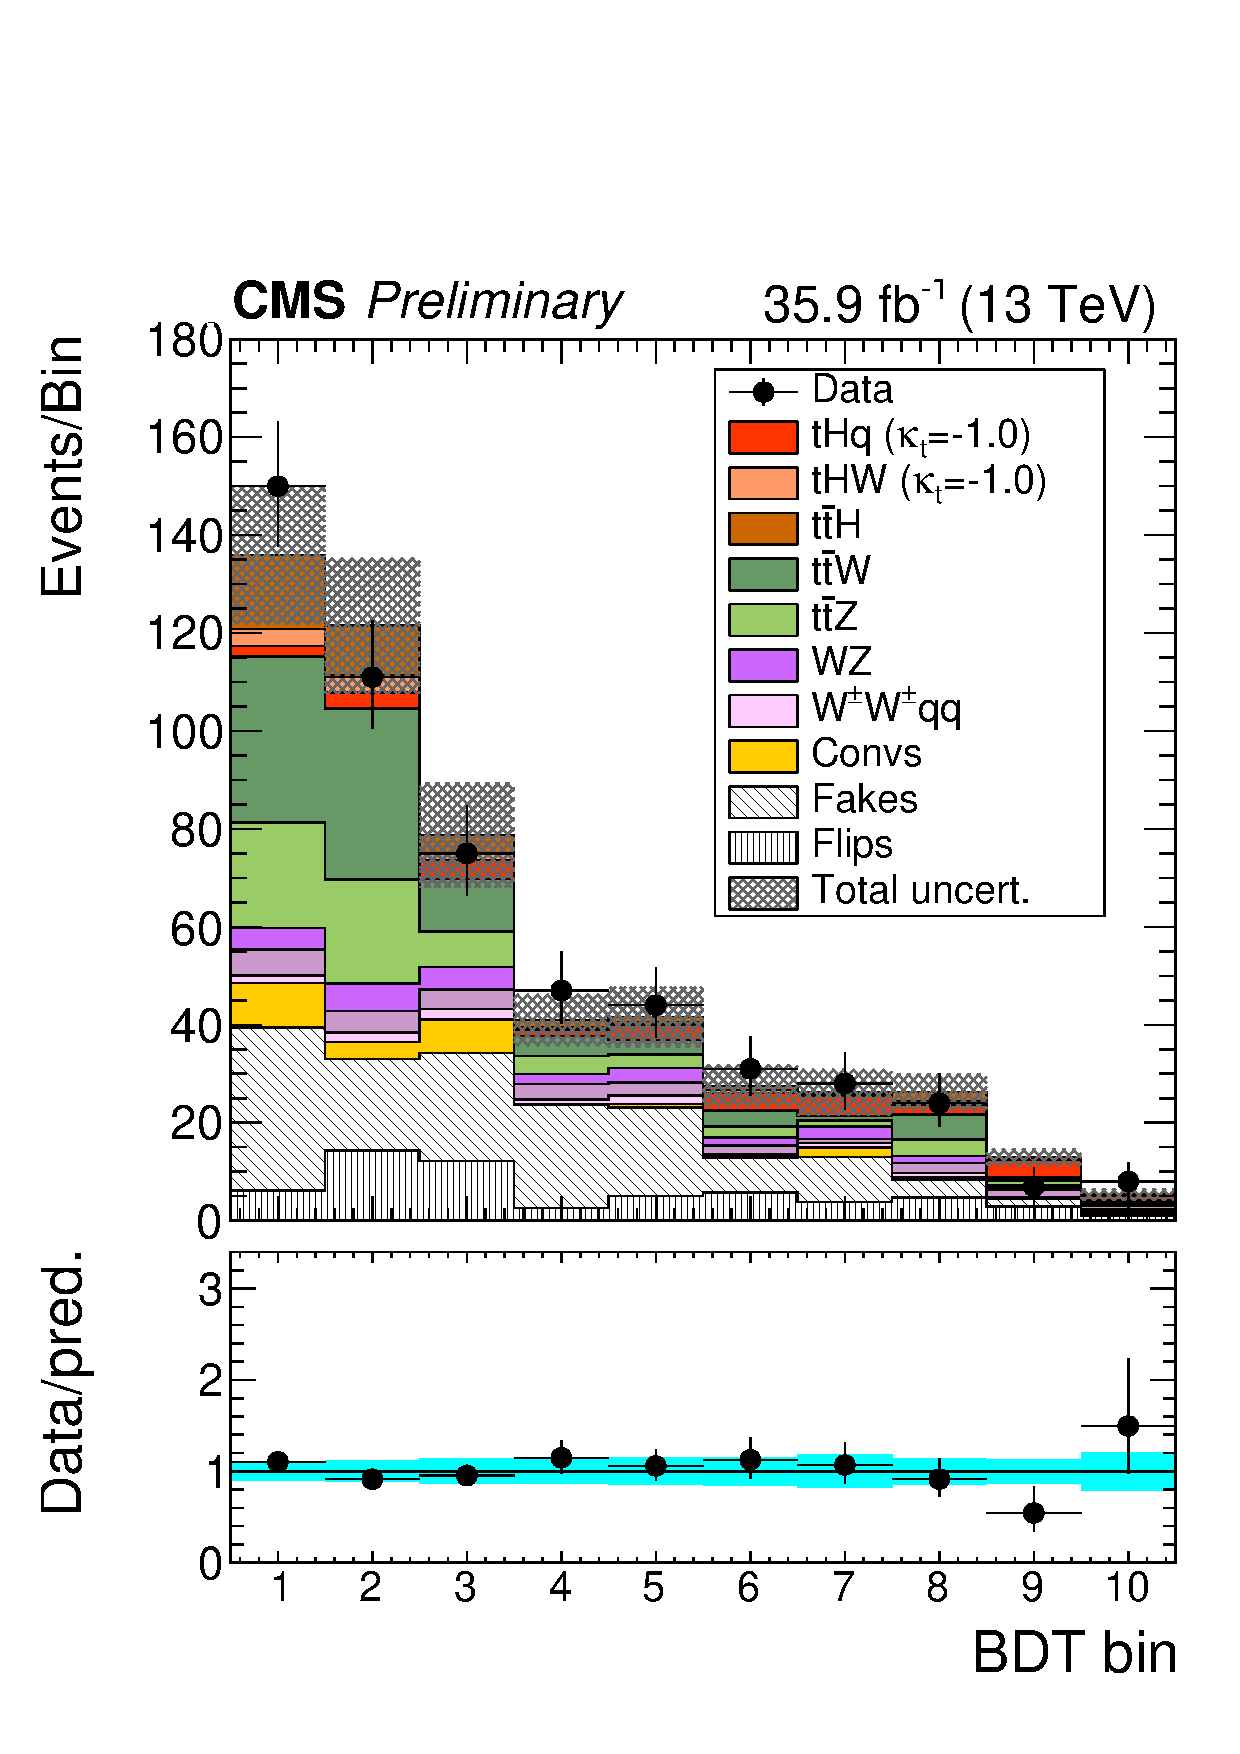
\includegraphics[width=0.32\textwidth]{figures/postfit/tHq_2lss_em_13TeV_prefit.pdf} \\
 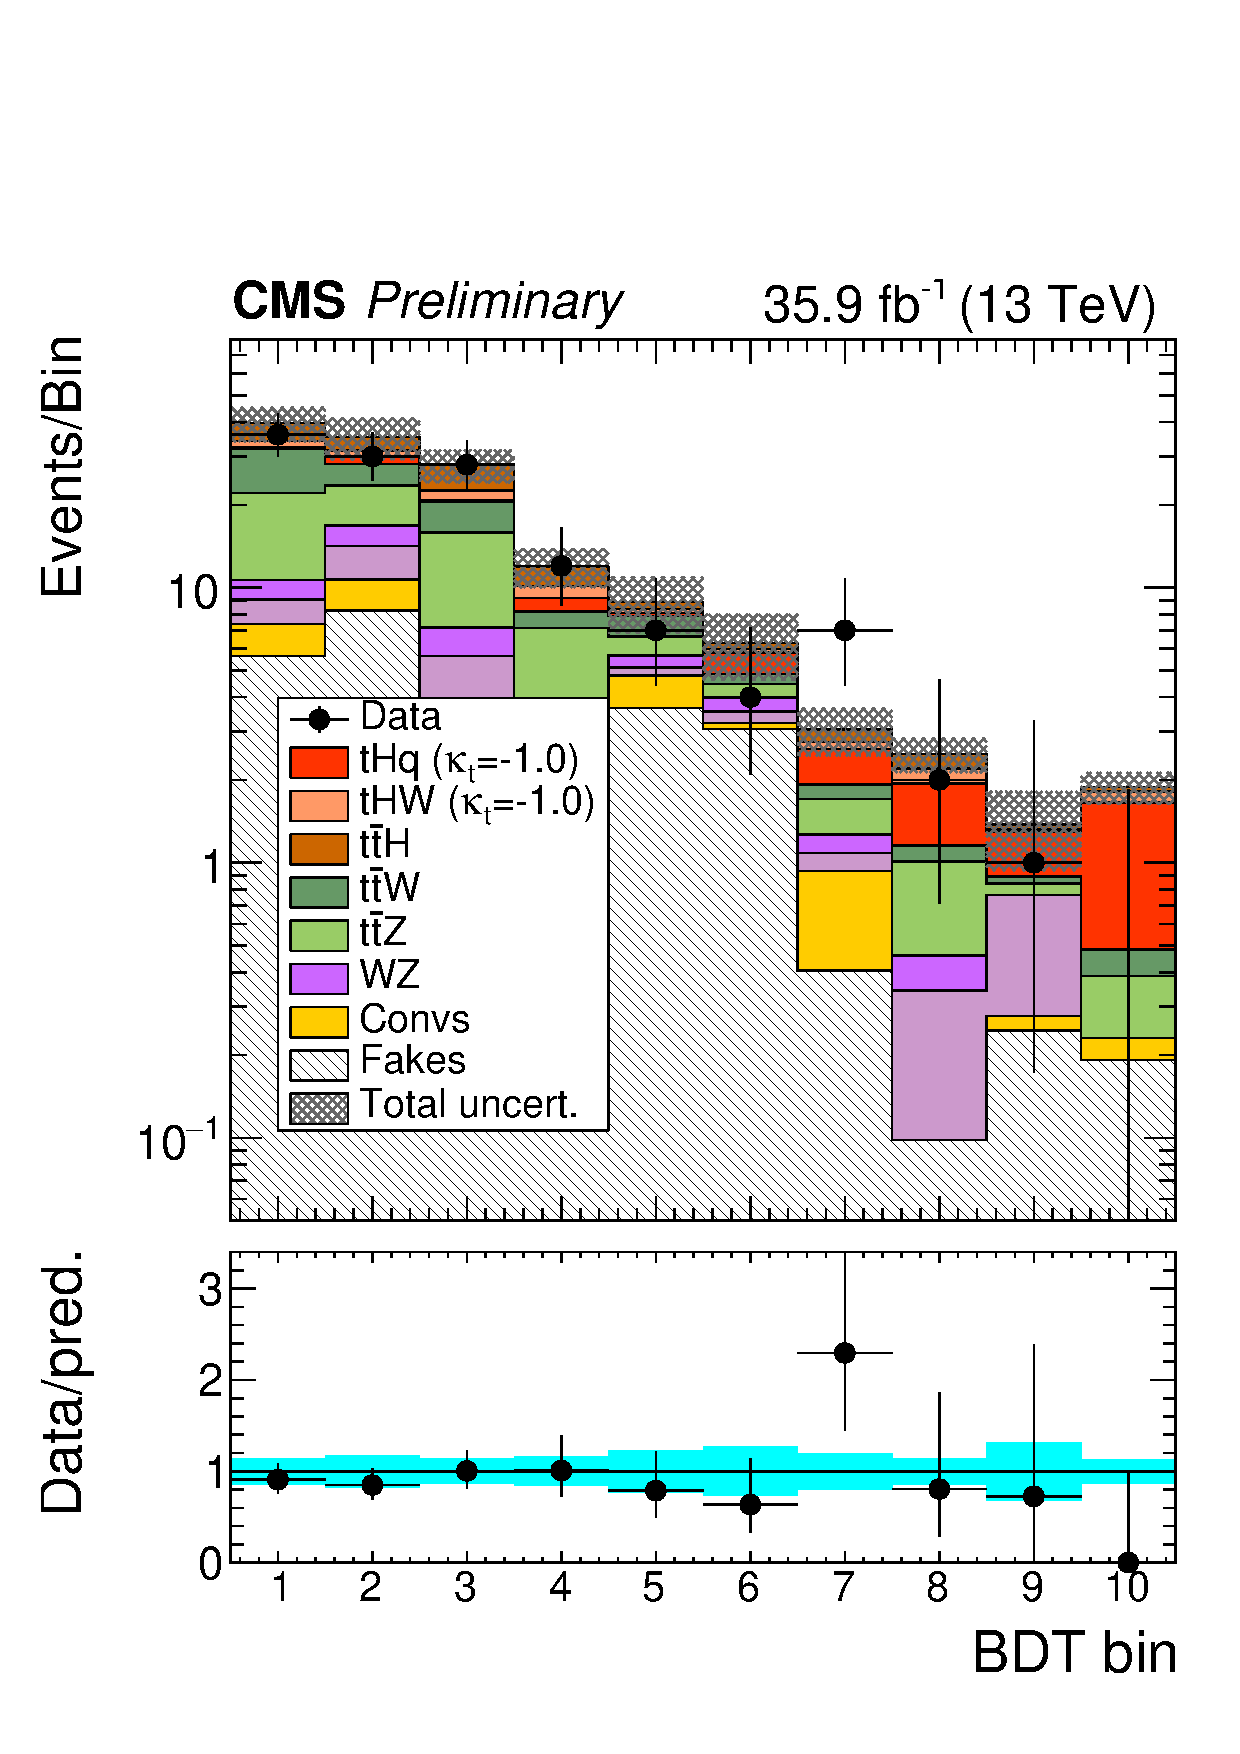
\includegraphics[width=0.32\textwidth]{figures/postfit/tHq_3l_13TeV_prefit_log.pdf}
 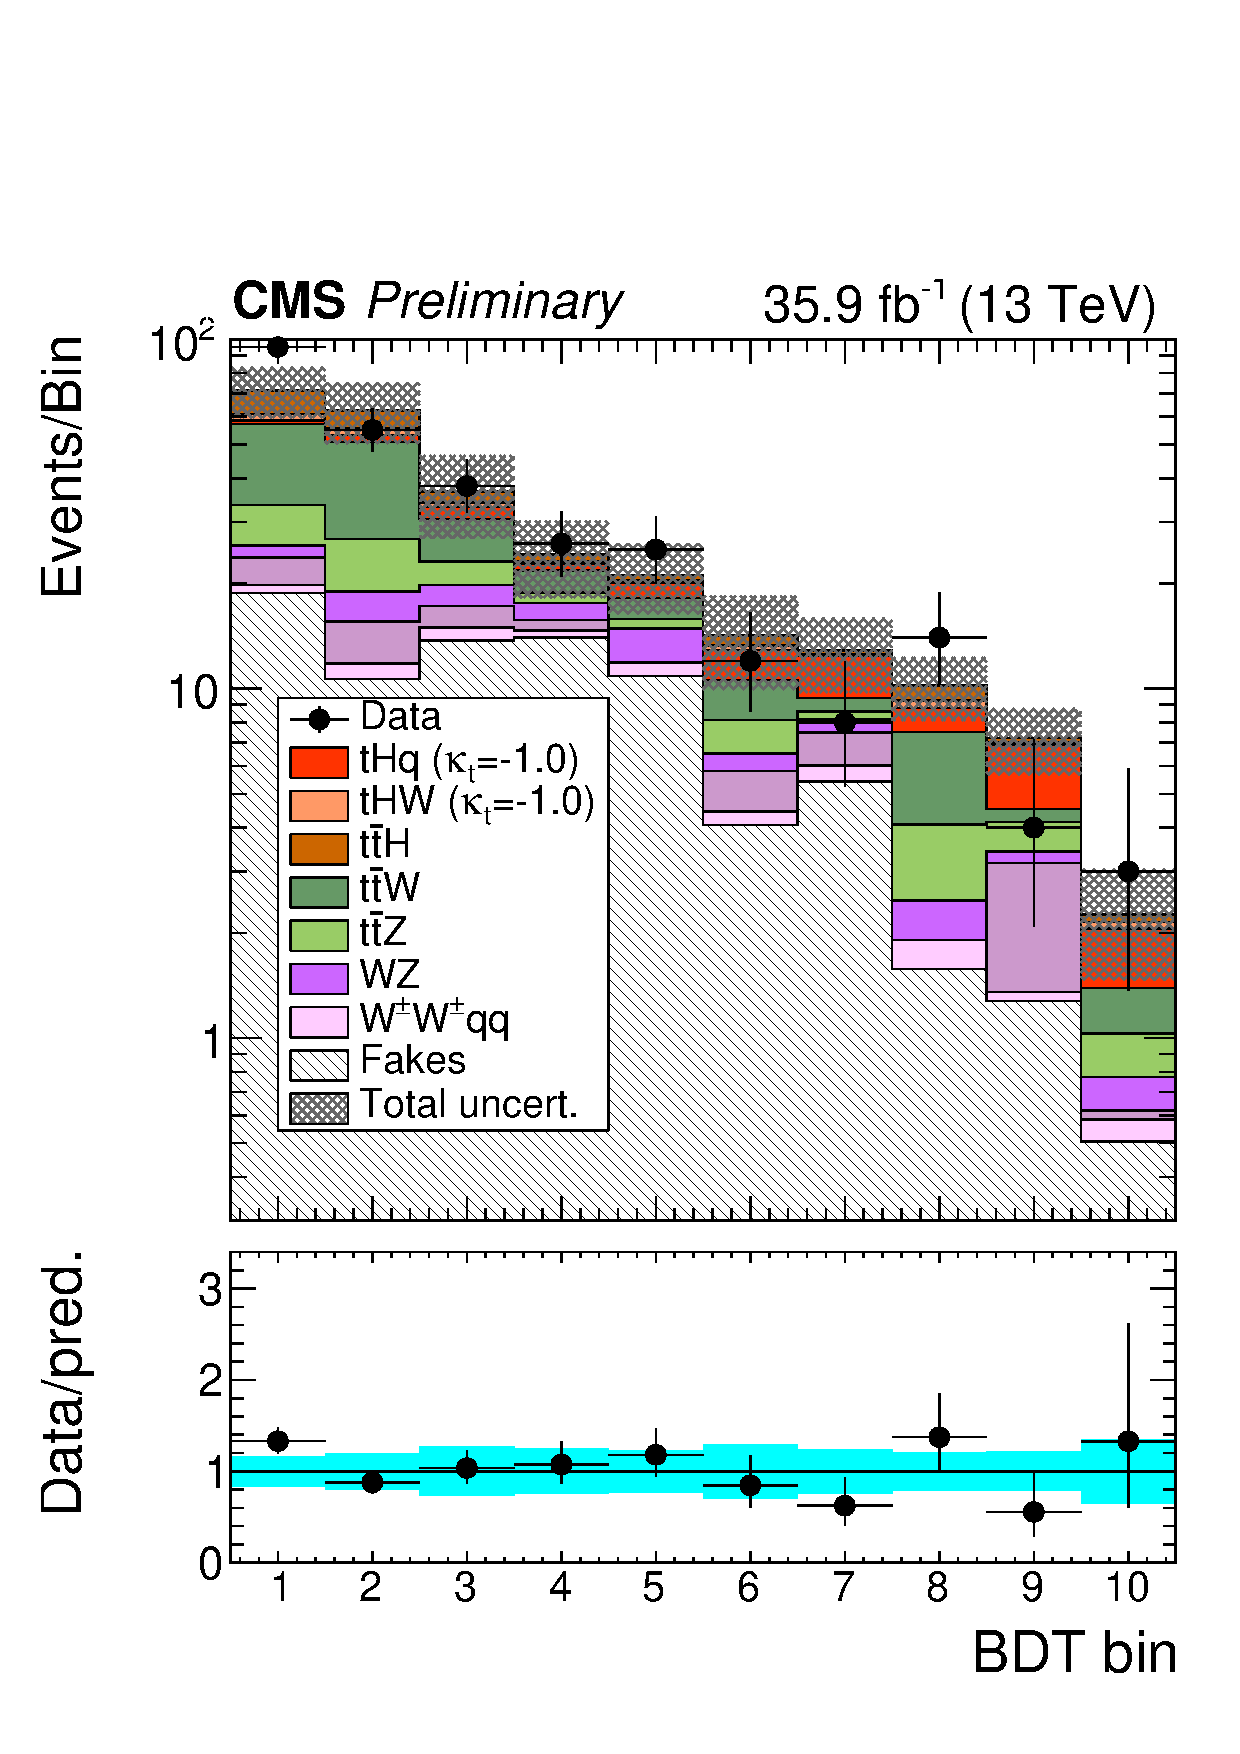
\includegraphics[width=0.32\textwidth]{figures/postfit/tHq_2lss_mm_13TeV_prefit_log.pdf}
 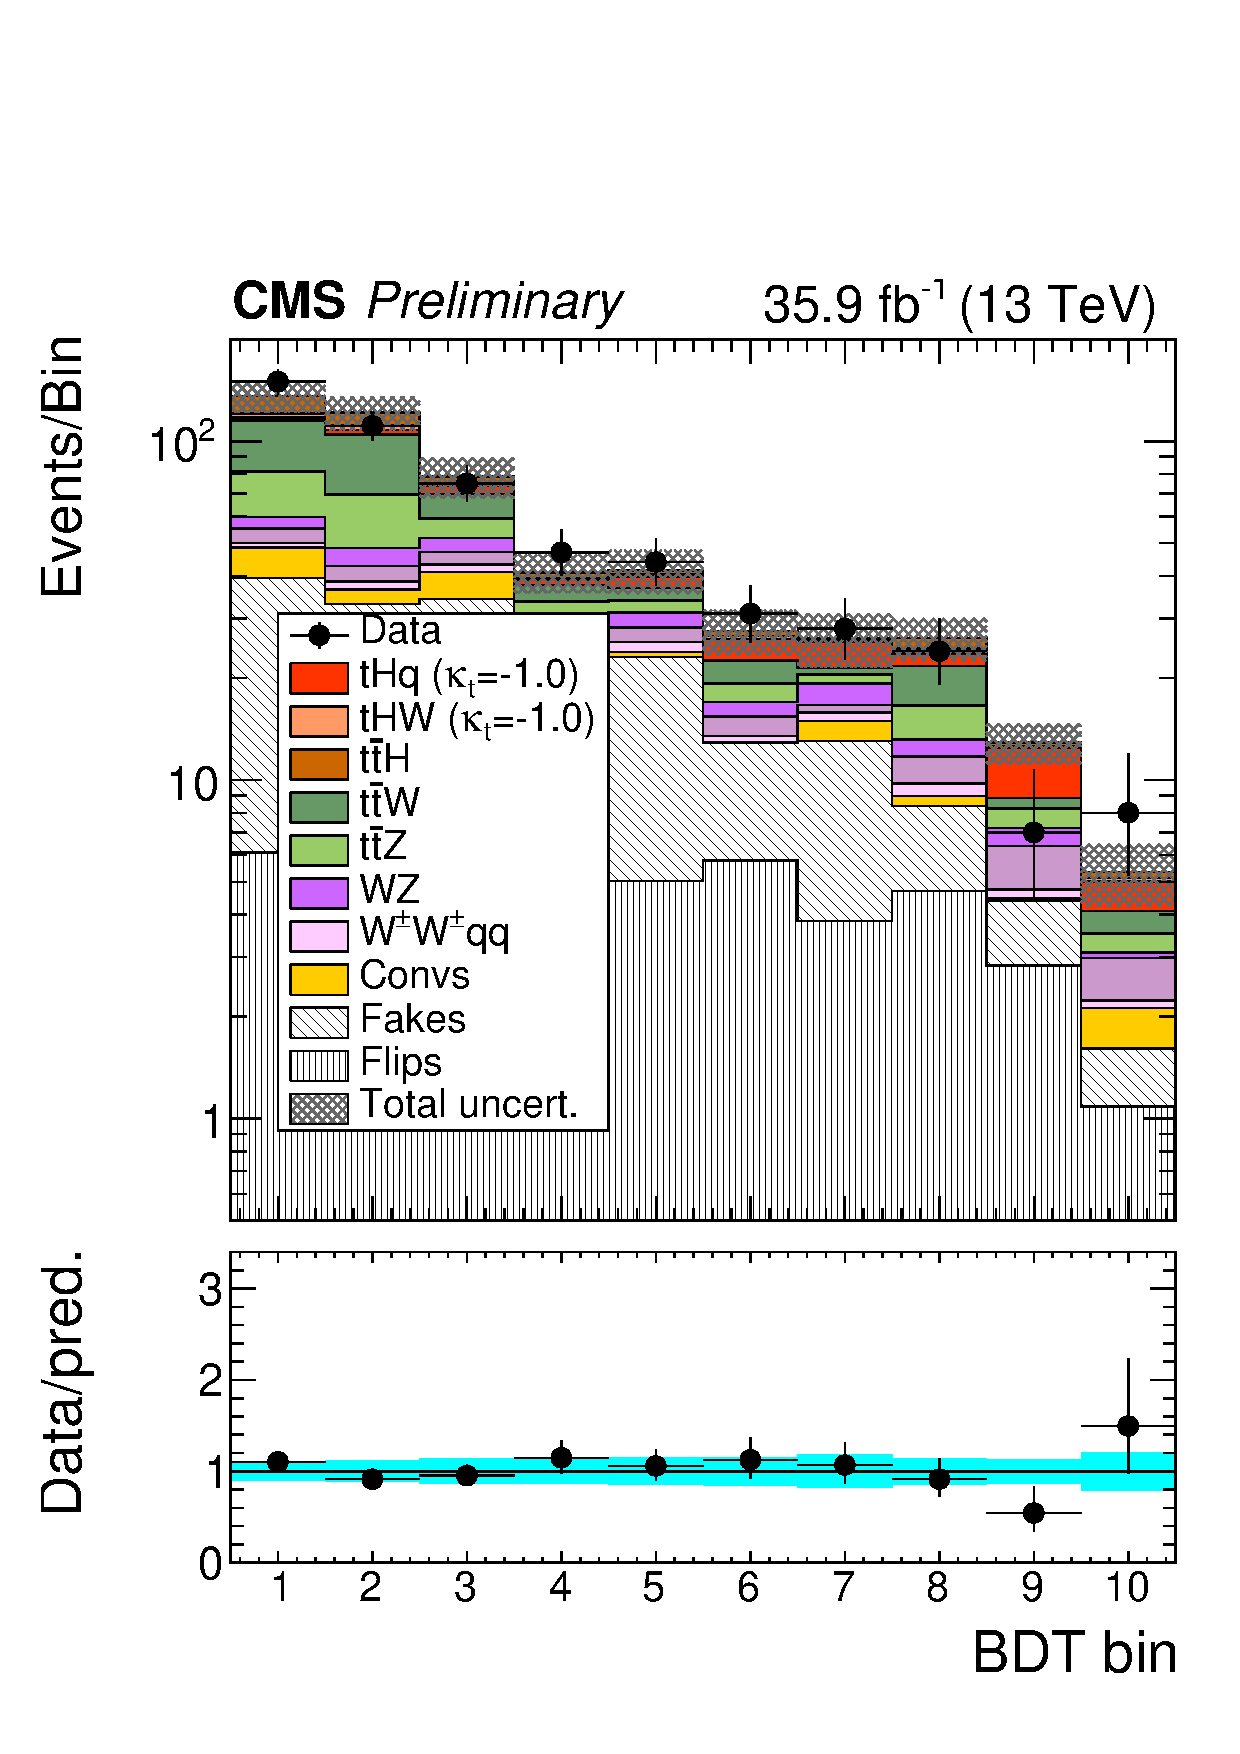
\includegraphics[width=0.32\textwidth]{figures/postfit/tHq_2lss_em_13TeV_prefit_log.pdf}
\caption{Expected (pre-fit) distributions in the final binning used for the signal extraction, for (from left to right) the three lepton channel, the \mumu\ channel, and the \emu\ channel. Linear scale (top row), and logarithmic scale (bottom row).}
\label{fig:finalbins}
\end{figure}

\begin{figure} [!h]
 \centering
 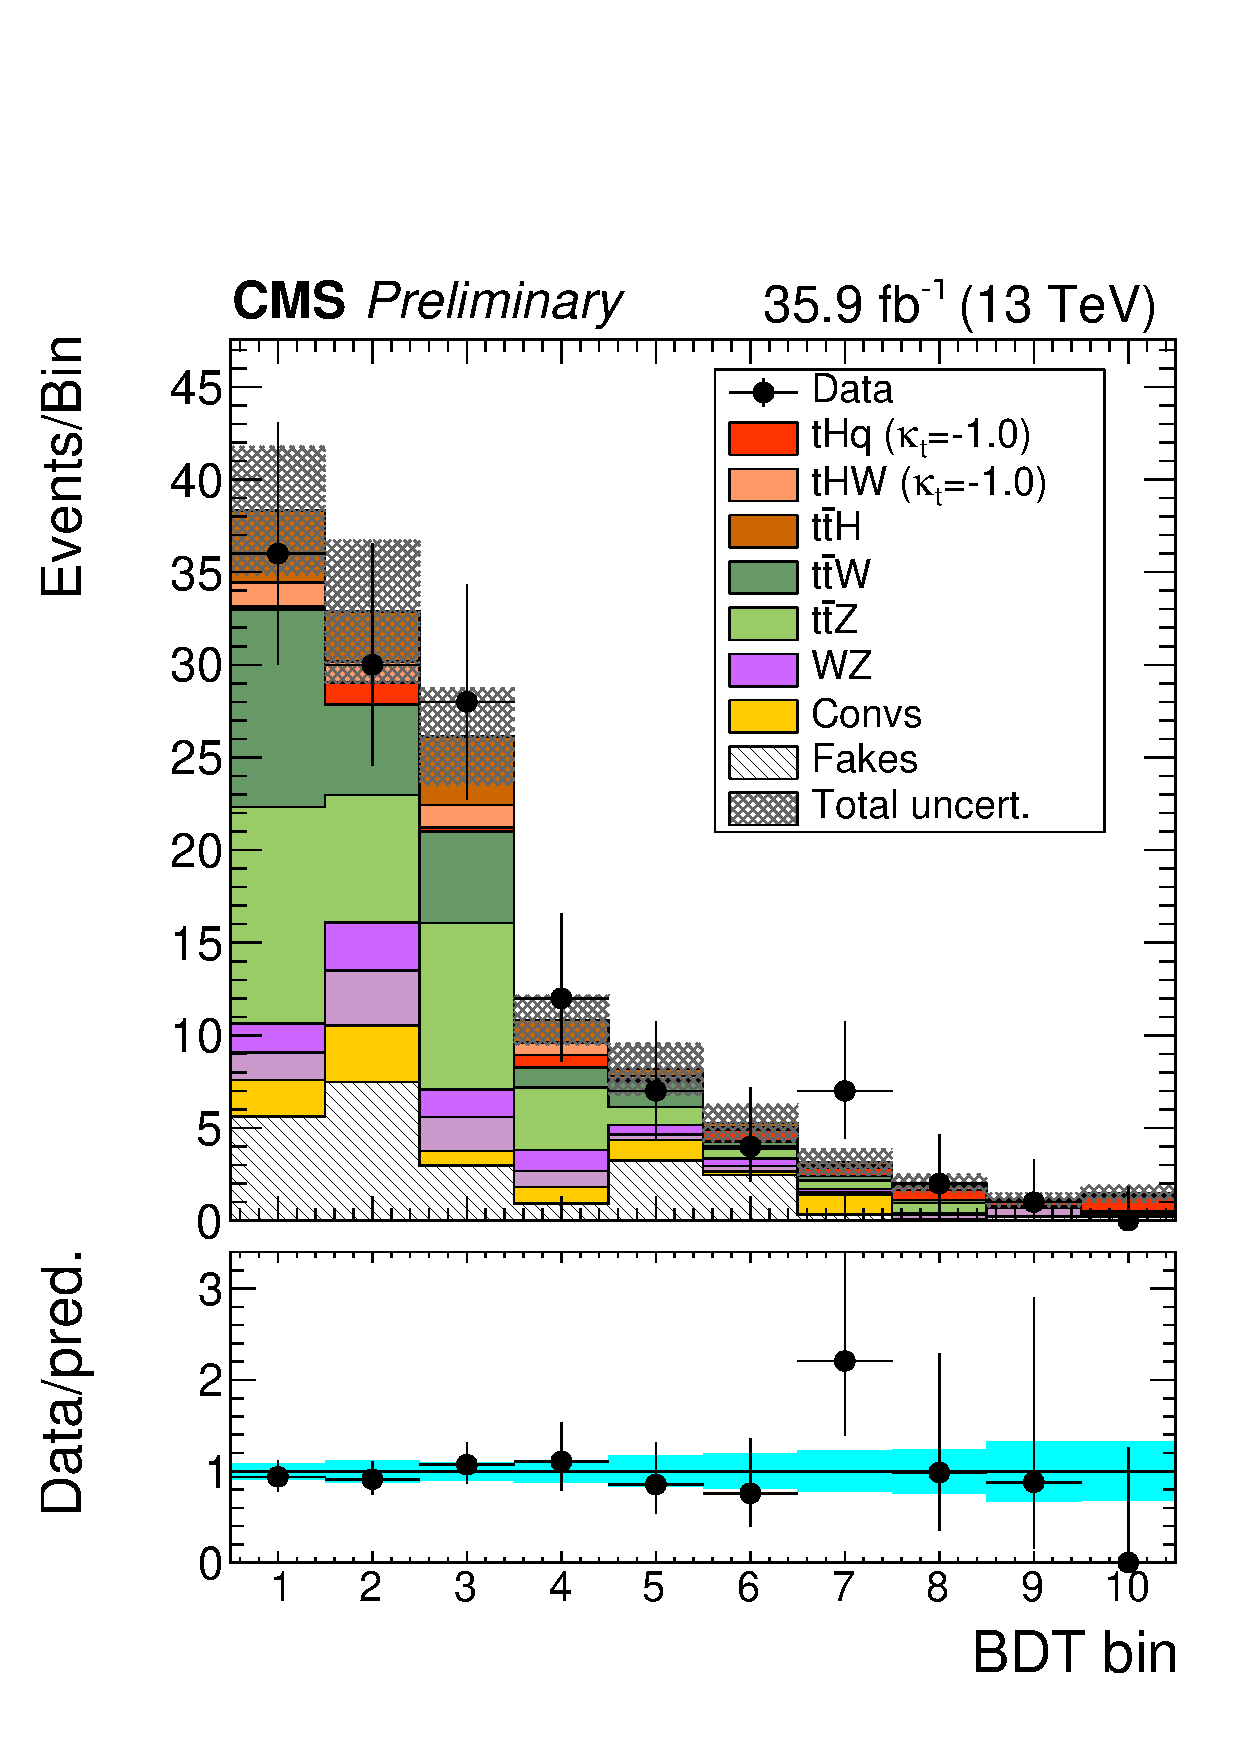
\includegraphics[width=0.32\textwidth]{figures/postfit/tHq_3l_13TeV_fit_s.pdf}
 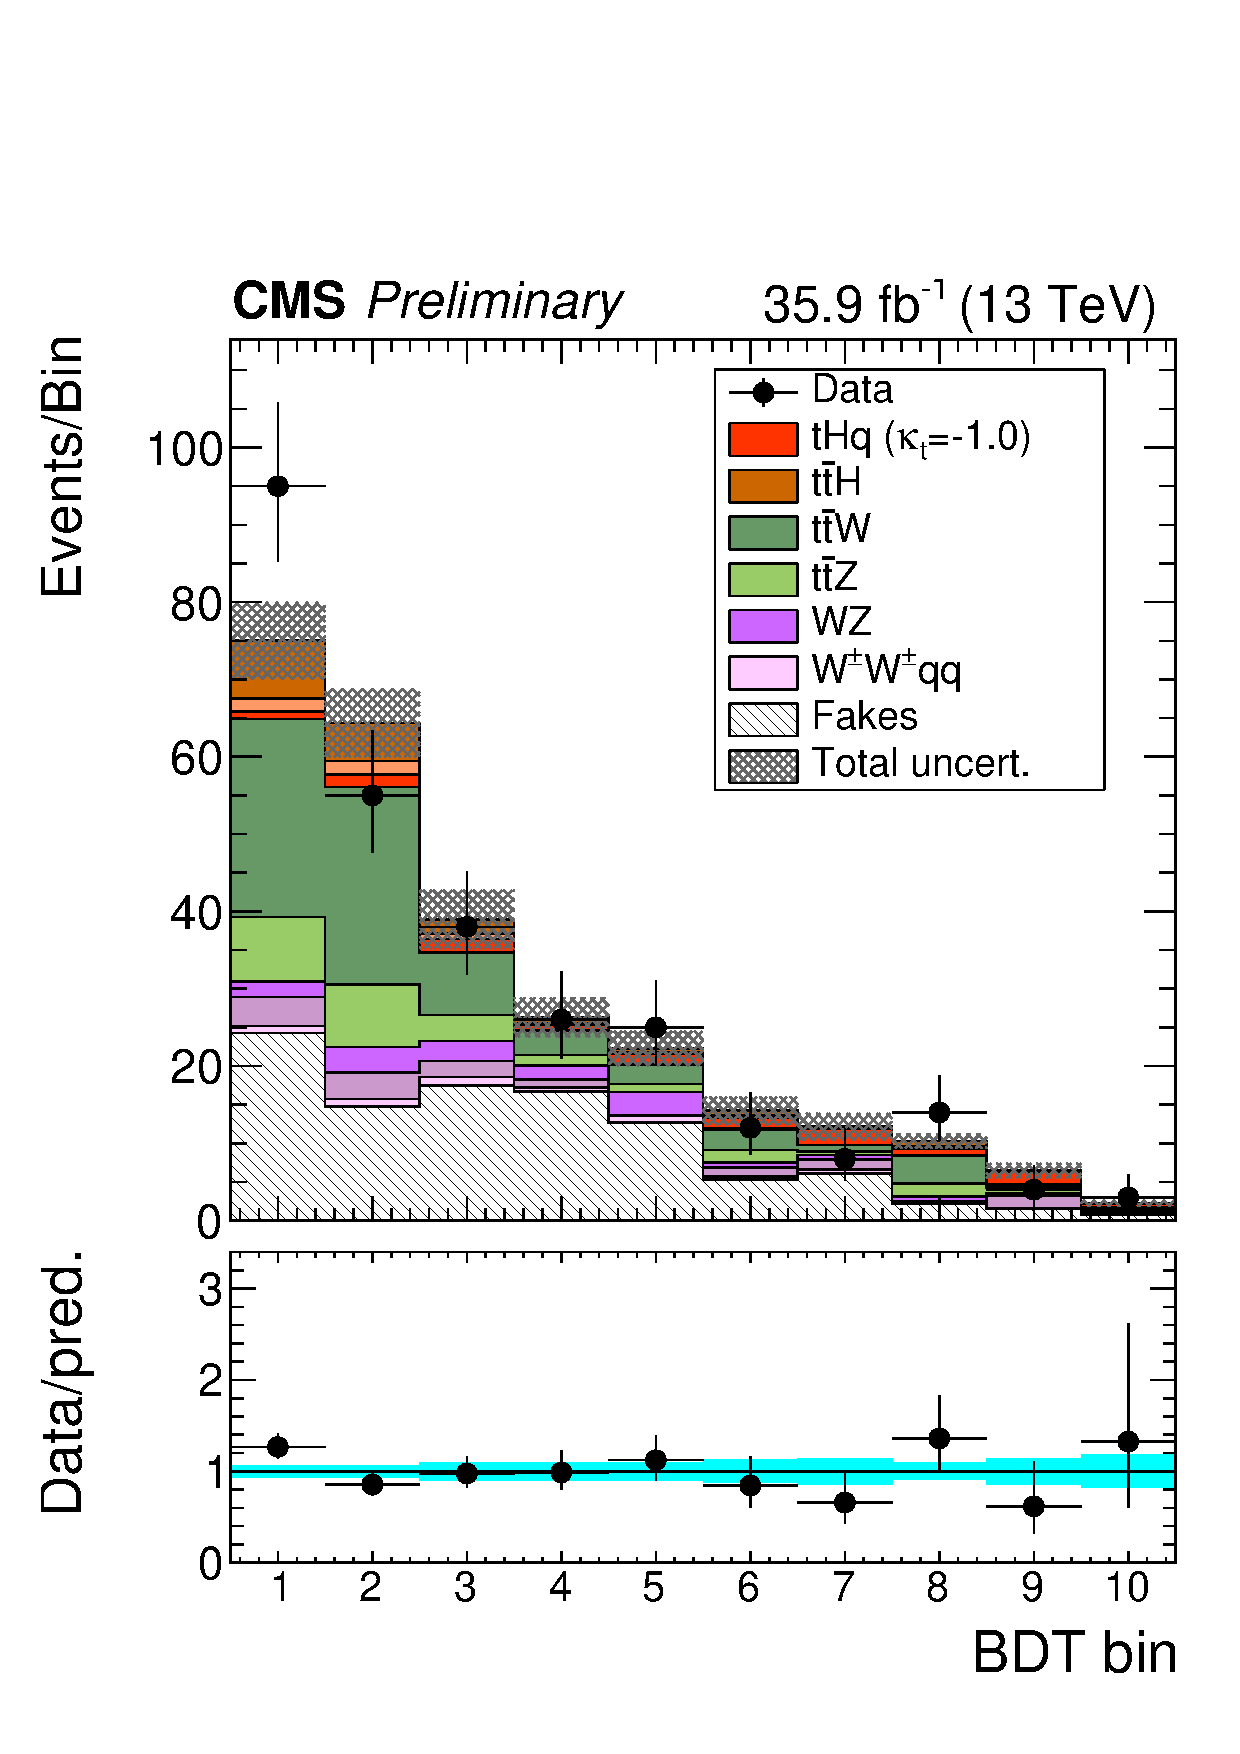
\includegraphics[width=0.32\textwidth]{figures/postfit/tHq_2lss_mm_13TeV_fit_s.pdf}
 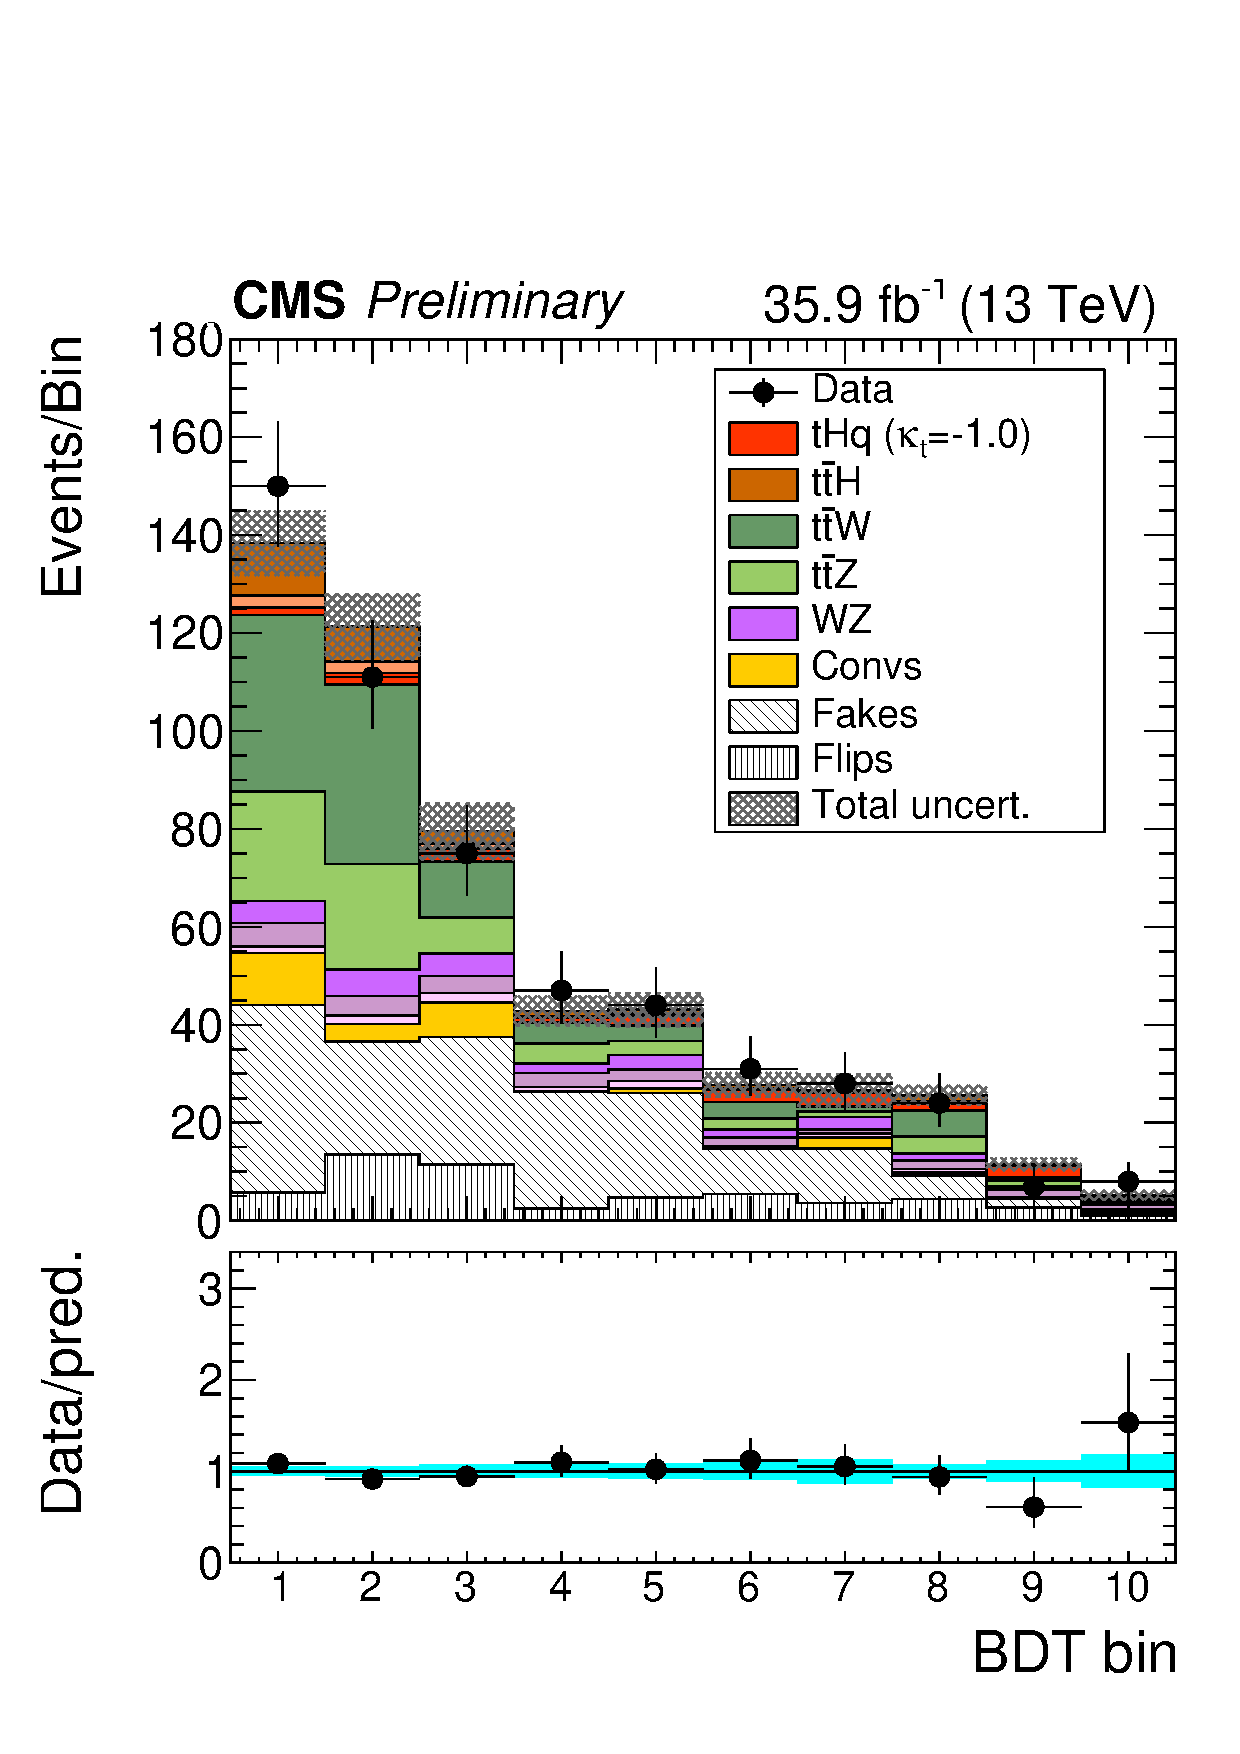
\includegraphics[width=0.32\textwidth]{figures/postfit/tHq_2lss_em_13TeV_fit_s.pdf} \\
 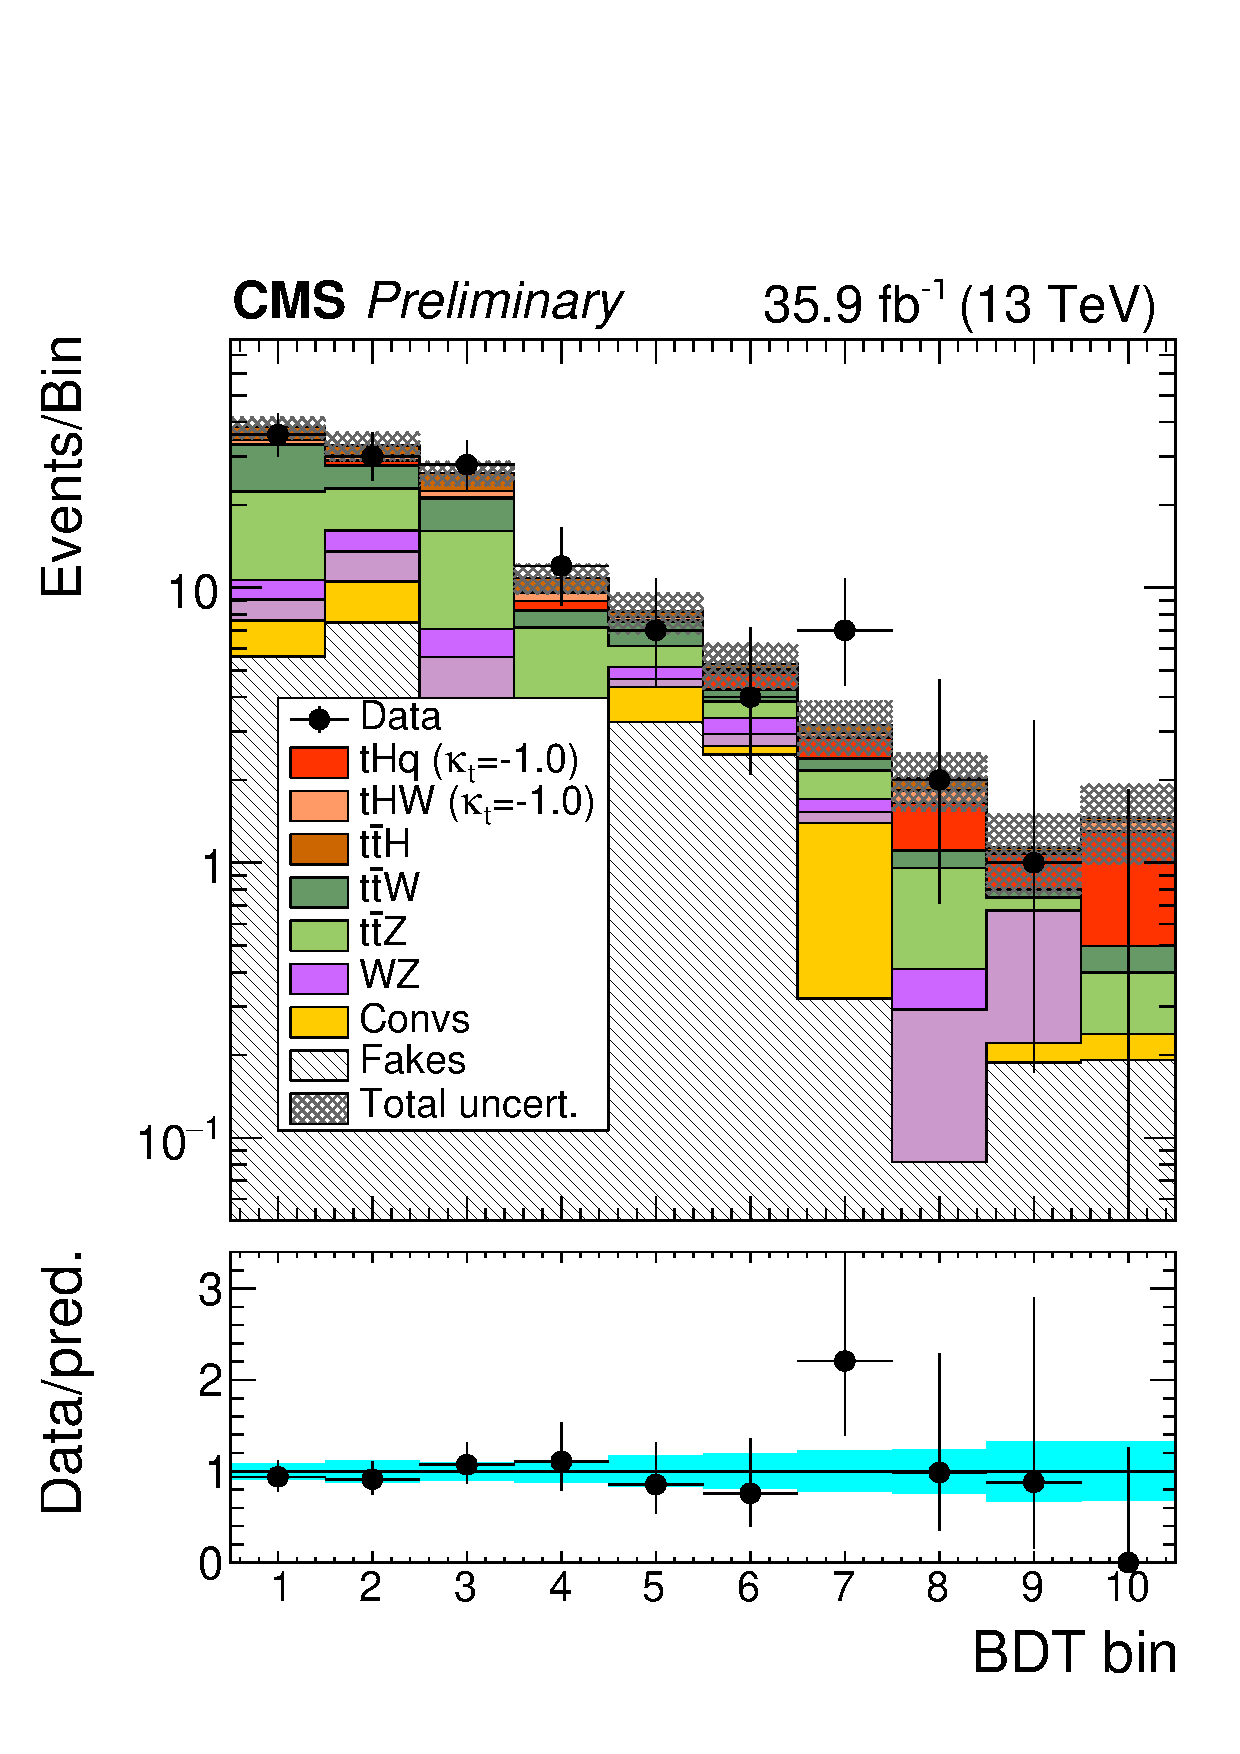
\includegraphics[width=0.32\textwidth]{figures/postfit/tHq_3l_13TeV_fit_s_log.pdf}
 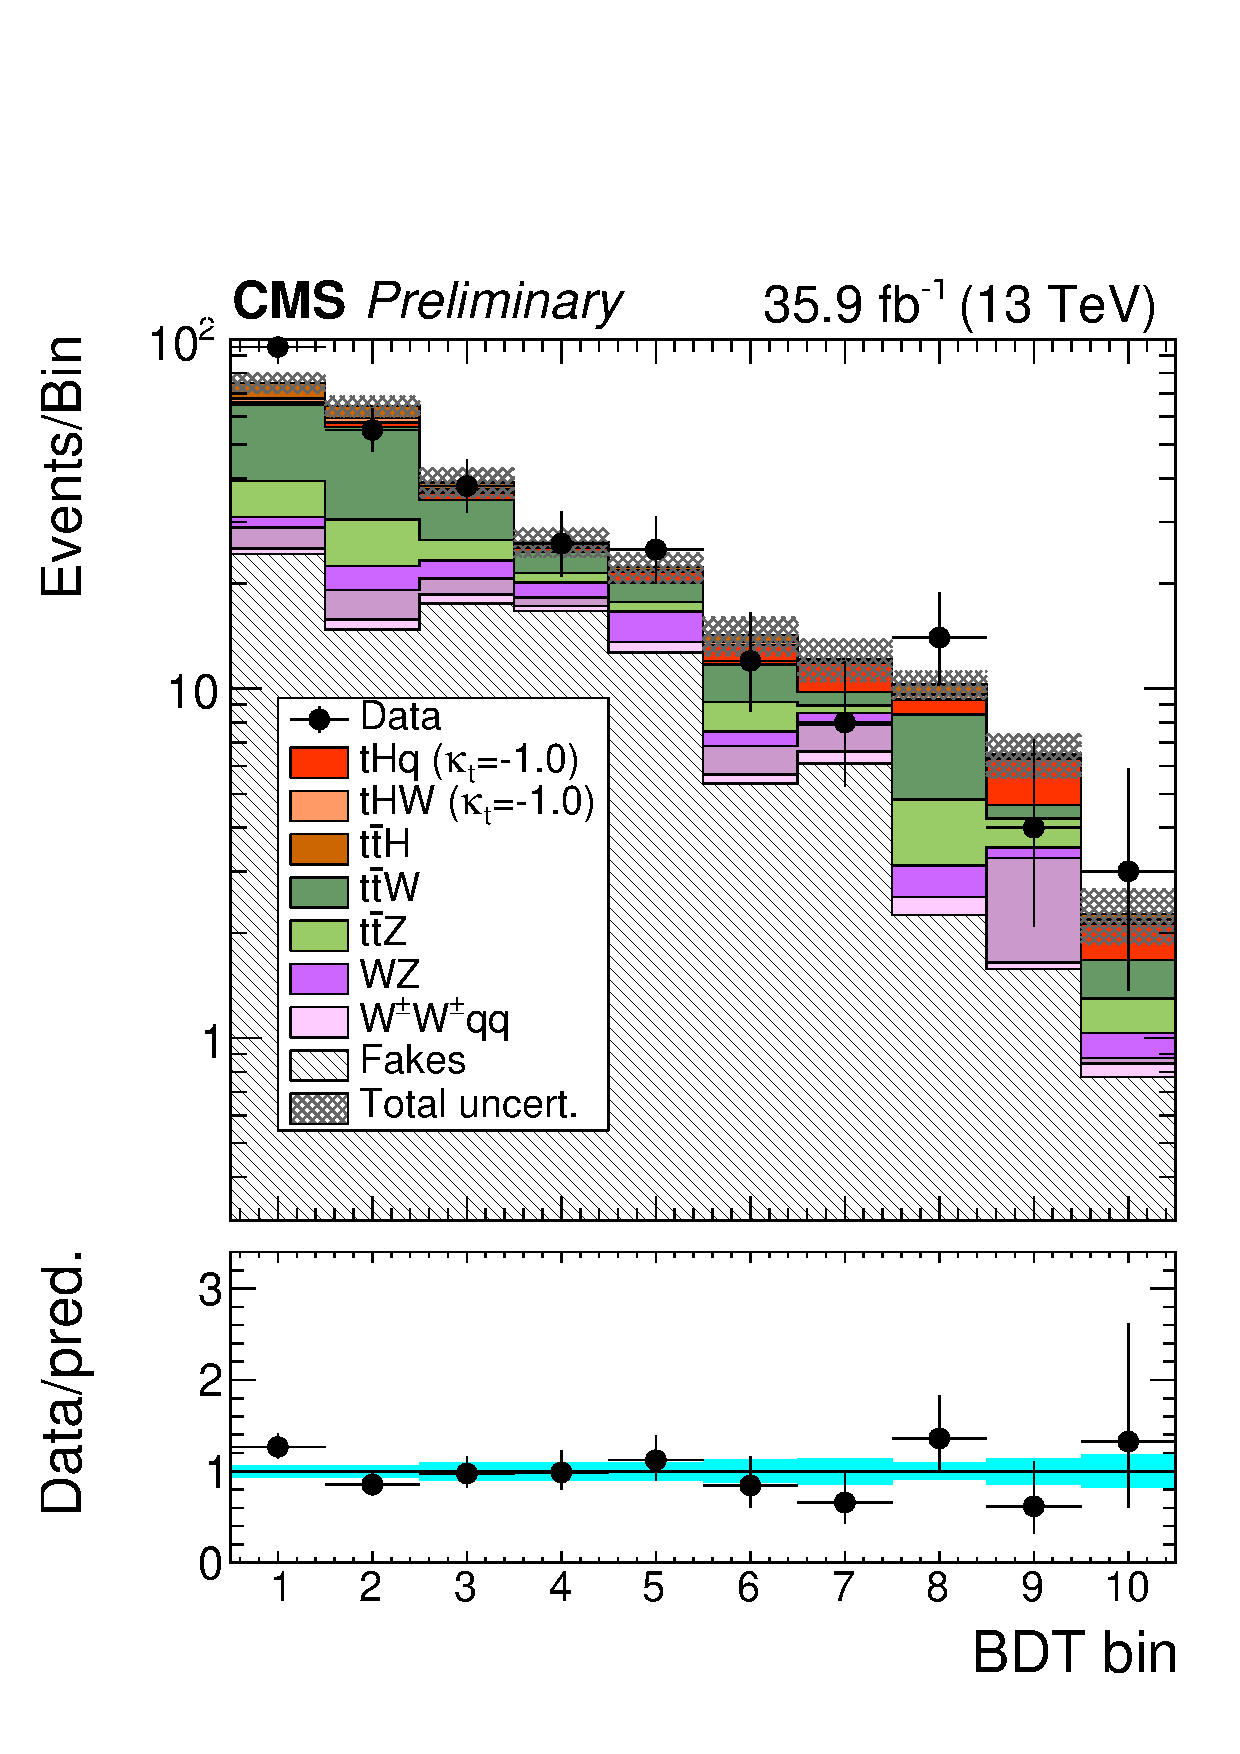
\includegraphics[width=0.32\textwidth]{figures/postfit/tHq_2lss_mm_13TeV_fit_s_log.pdf}
 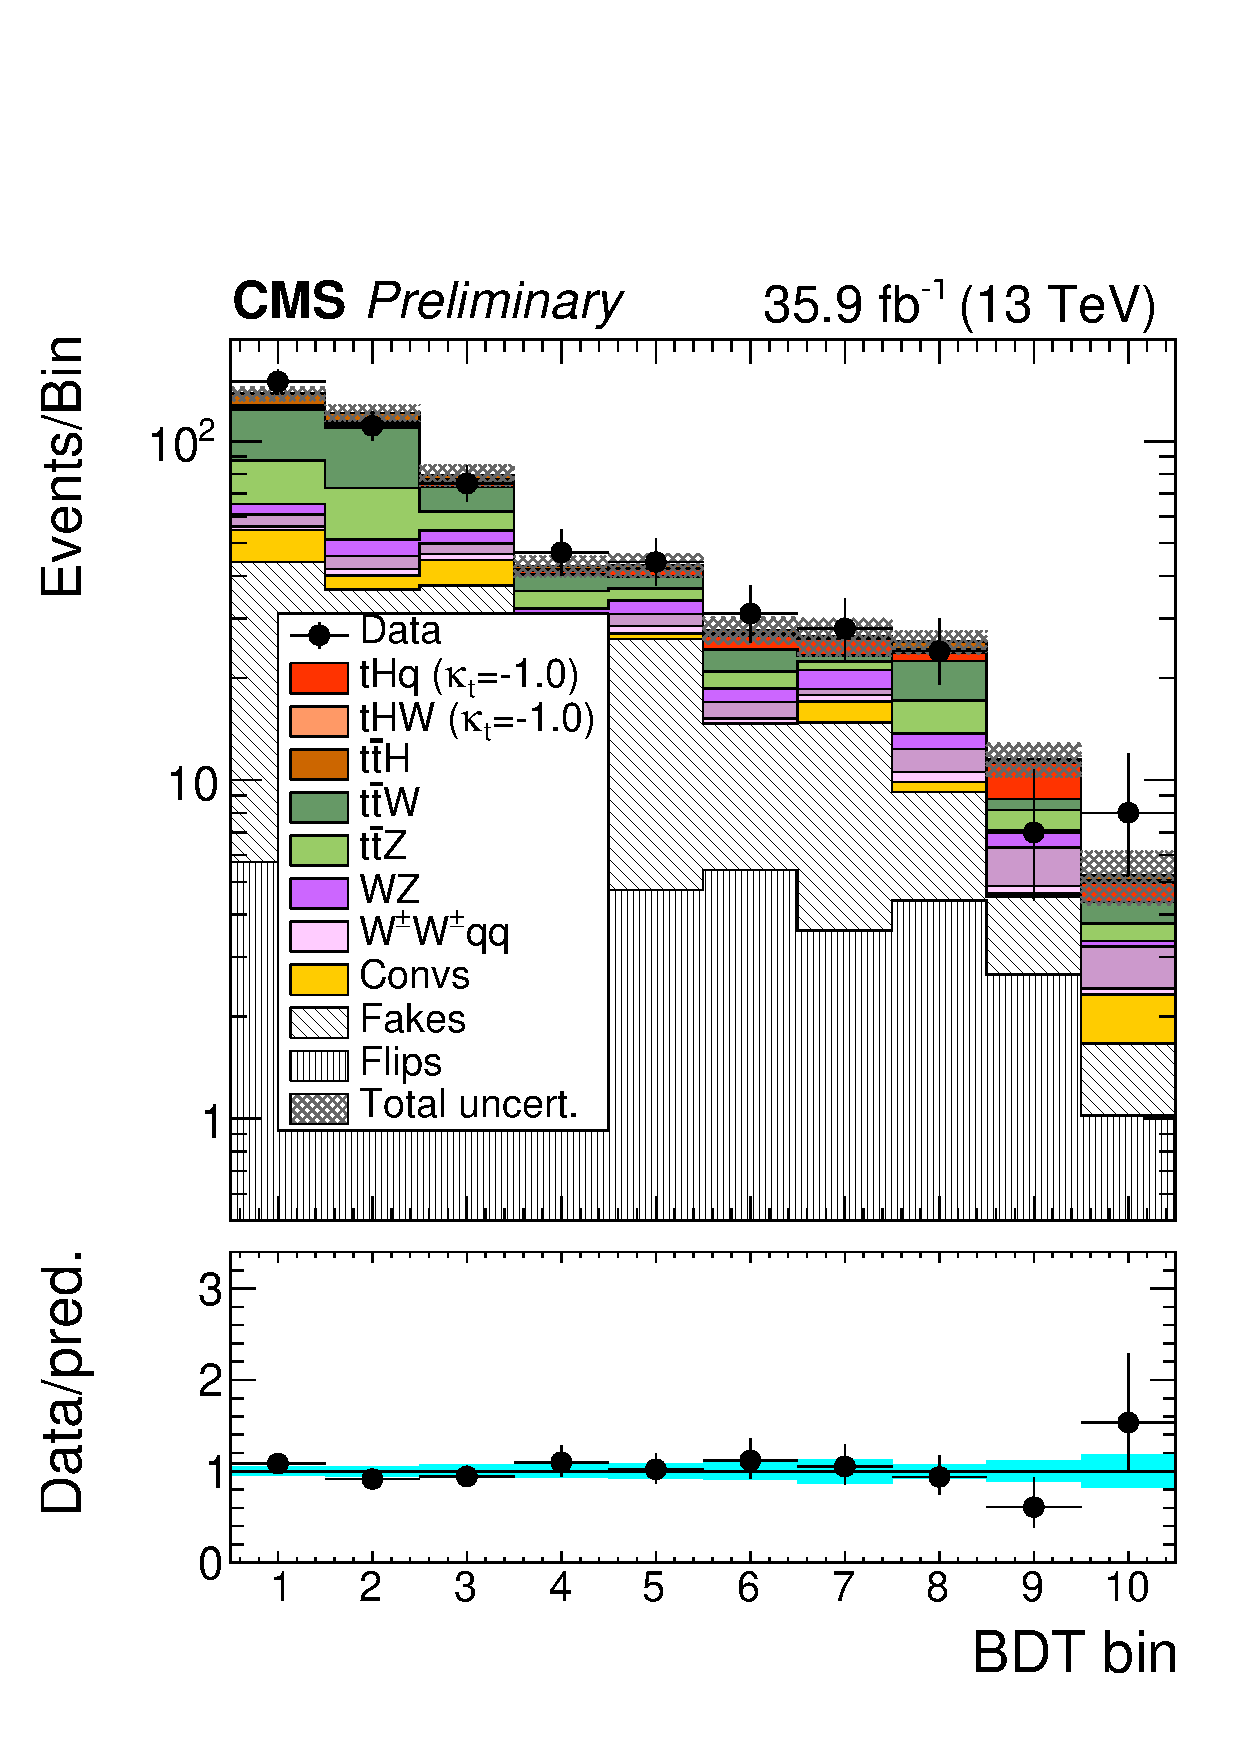
\includegraphics[width=0.32\textwidth]{figures/postfit/tHq_2lss_em_13TeV_fit_s_log.pdf}
\caption{Post-fit distributions in the final binning used for the signal extraction, for (from left to right) the three lepton channel, the \mumu\ channel, and the \emu\ channel. Linear scale (top row), and logarithmic scale (bottom row).}
\label{fig:postfit}
\end{figure}

\begin{figure} [!h]
 \centering
 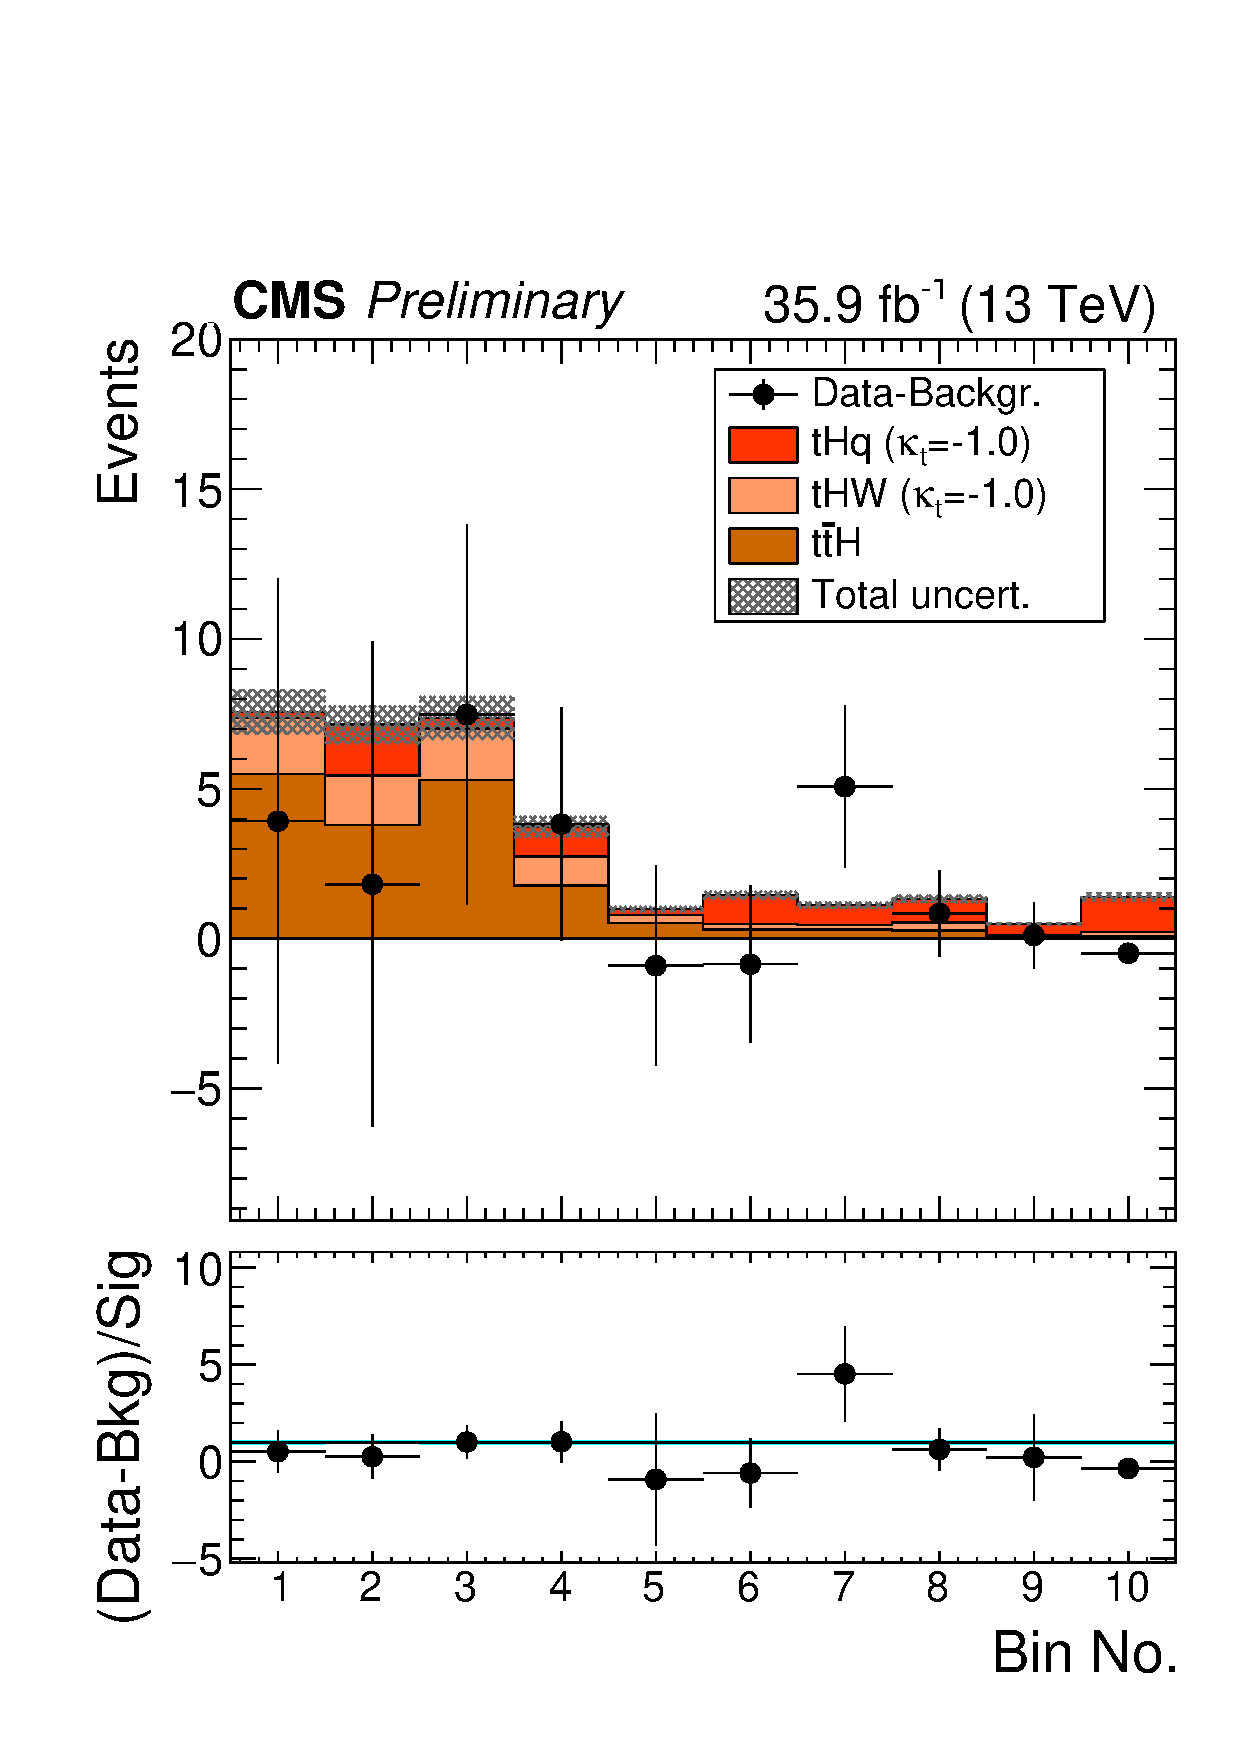
\includegraphics[width=0.32\textwidth]{figures/postfit/bgsub/ITC/tHq_3l_13TeV_prefit.pdf}
 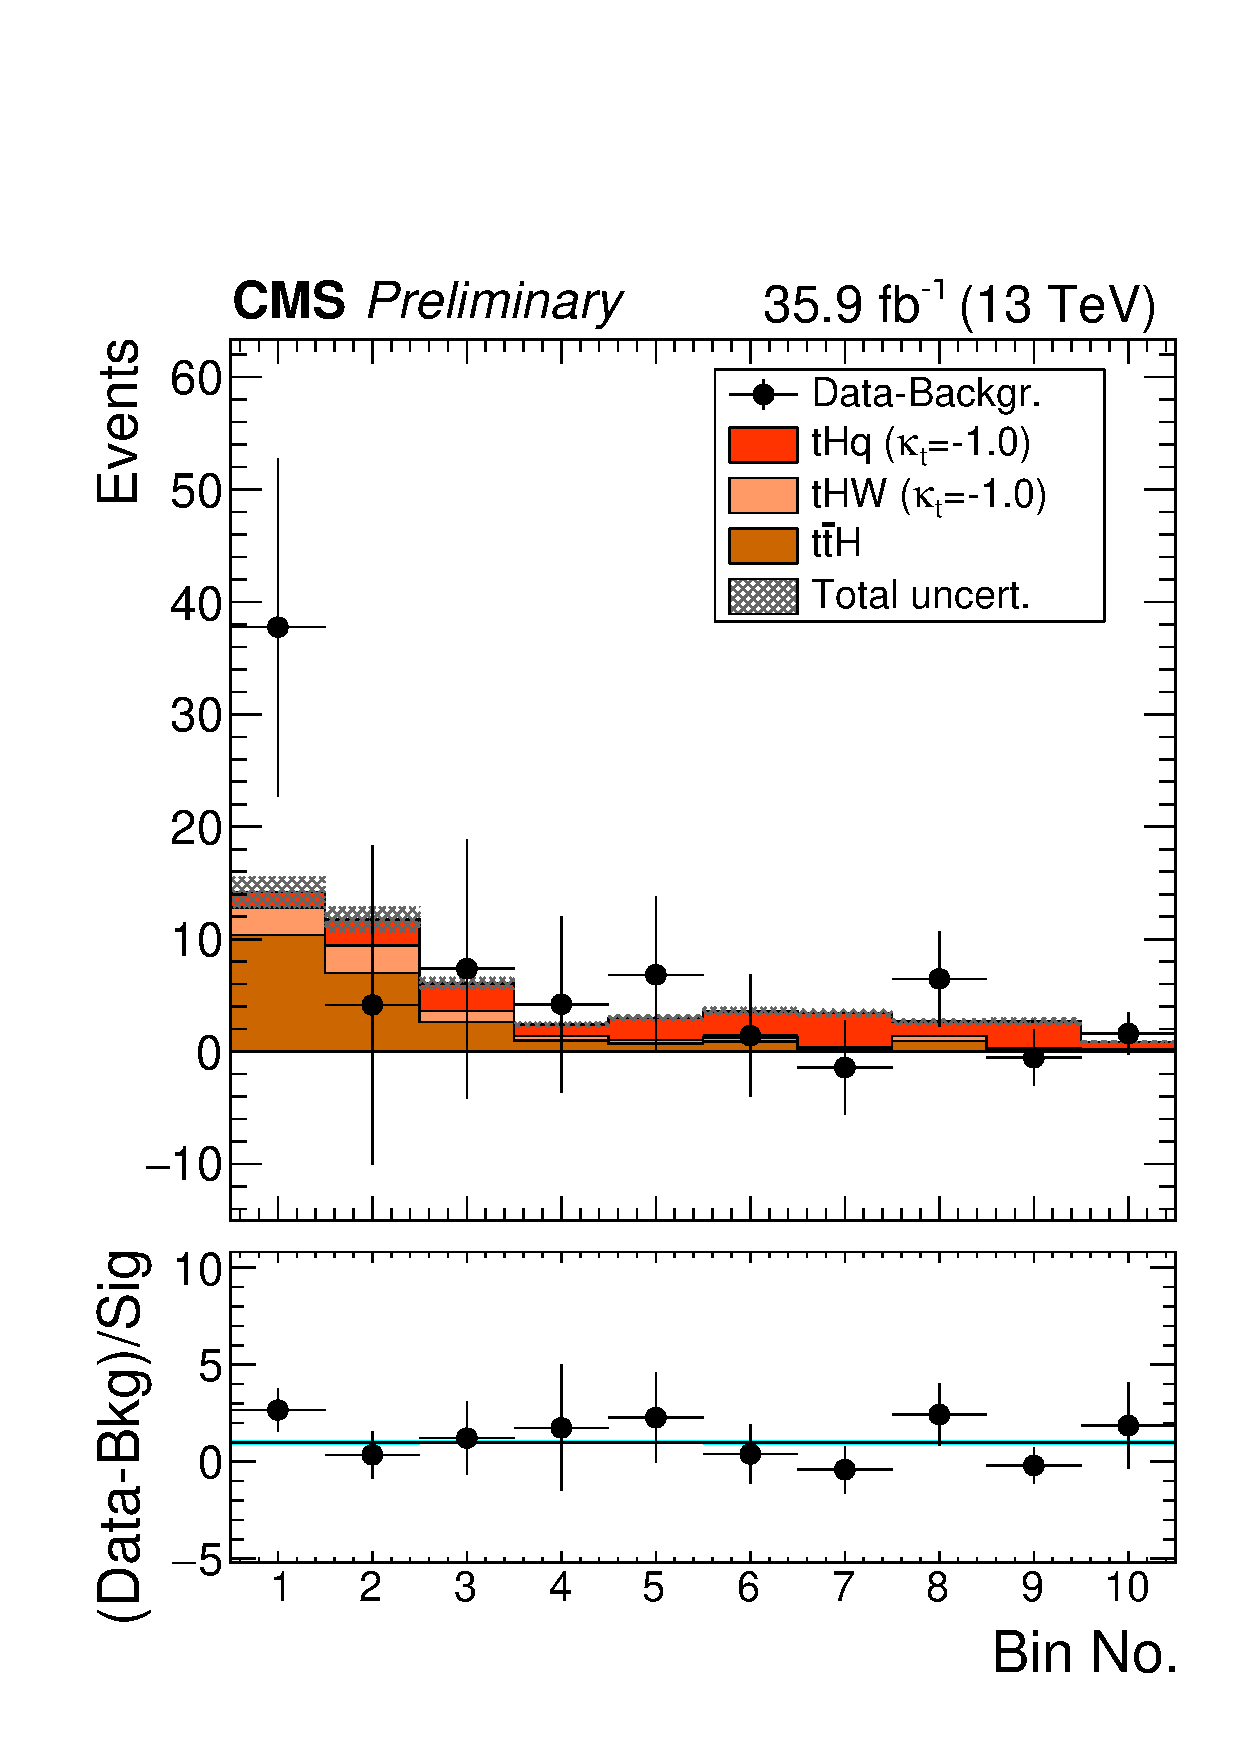
\includegraphics[width=0.32\textwidth]{figures/postfit/bgsub/ITC/tHq_2lss_mm_13TeV_prefit.pdf}
 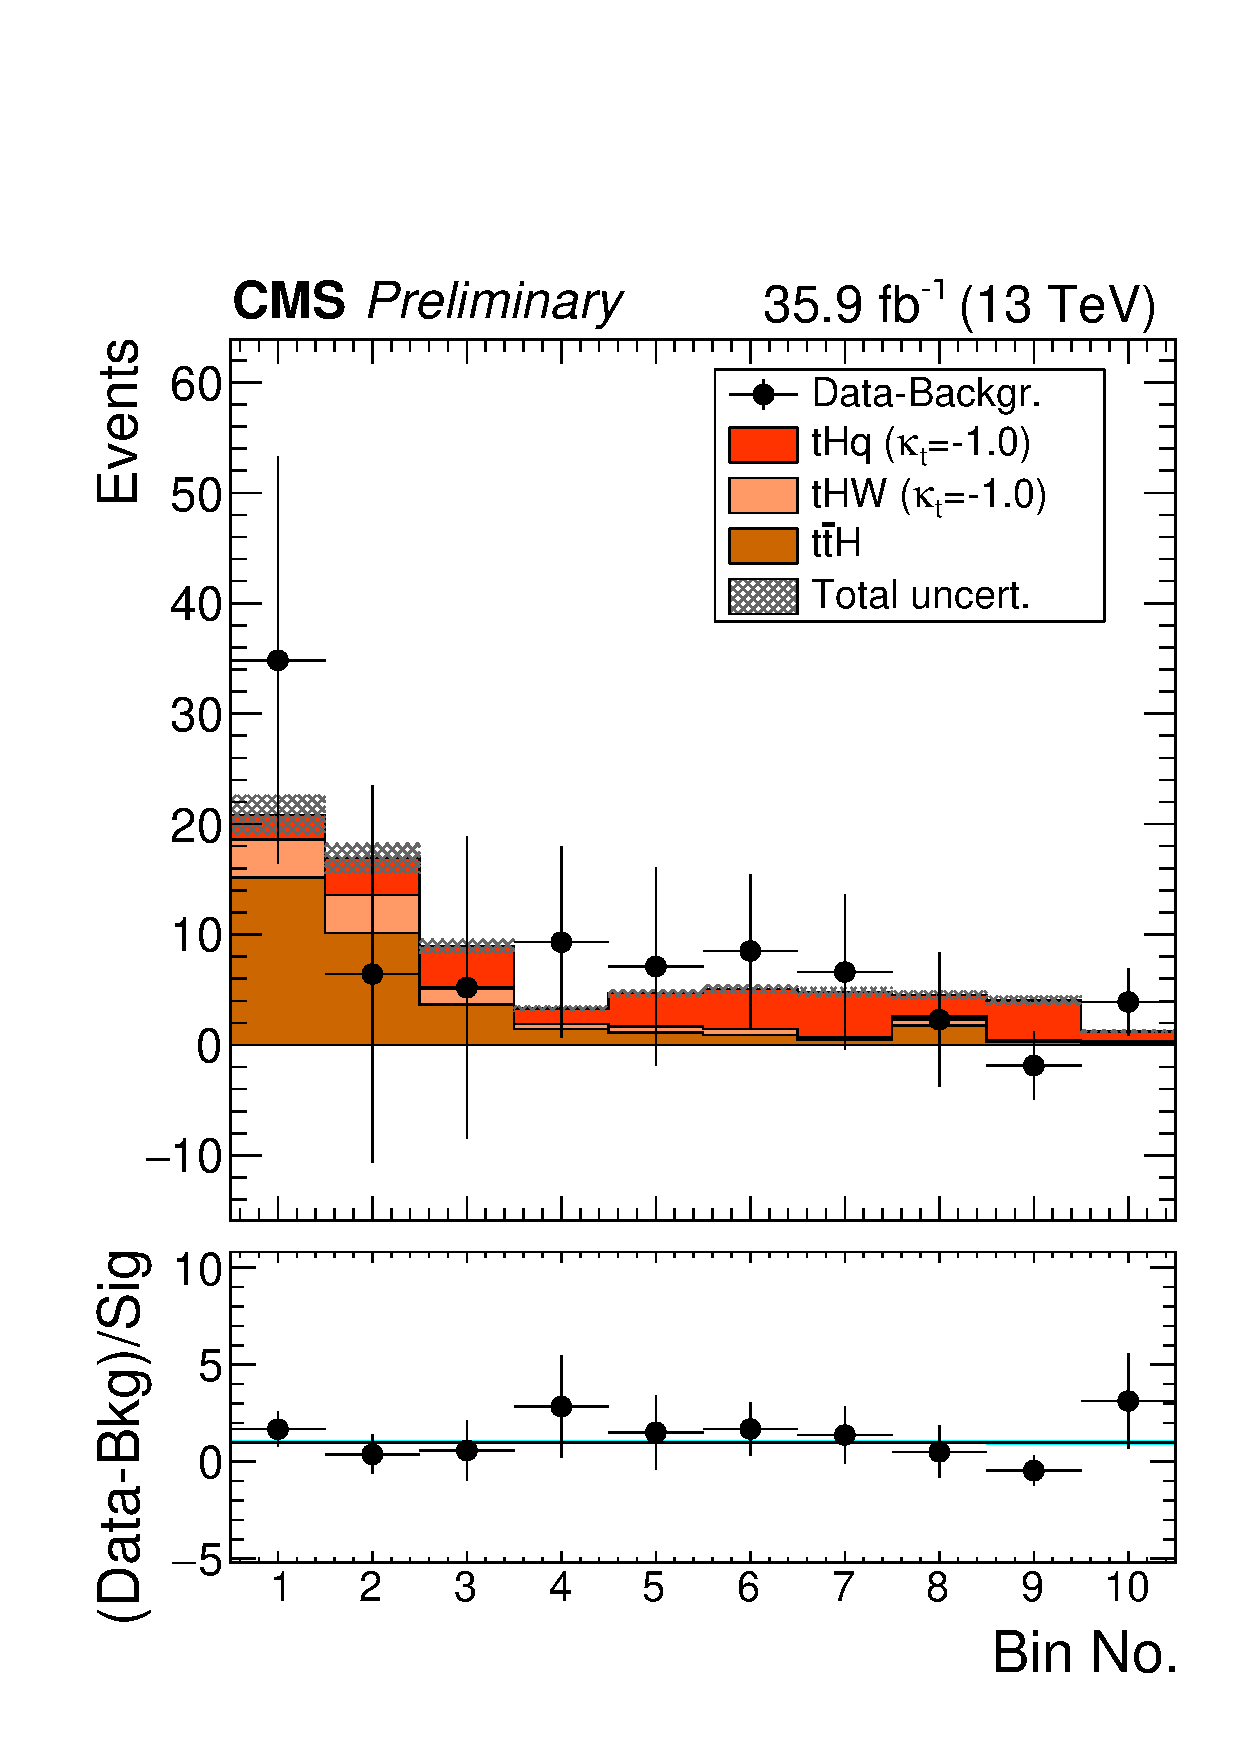
\includegraphics[width=0.32\textwidth]{figures/postfit/bgsub/ITC/tHq_2lss_em_13TeV_prefit.pdf} \\
 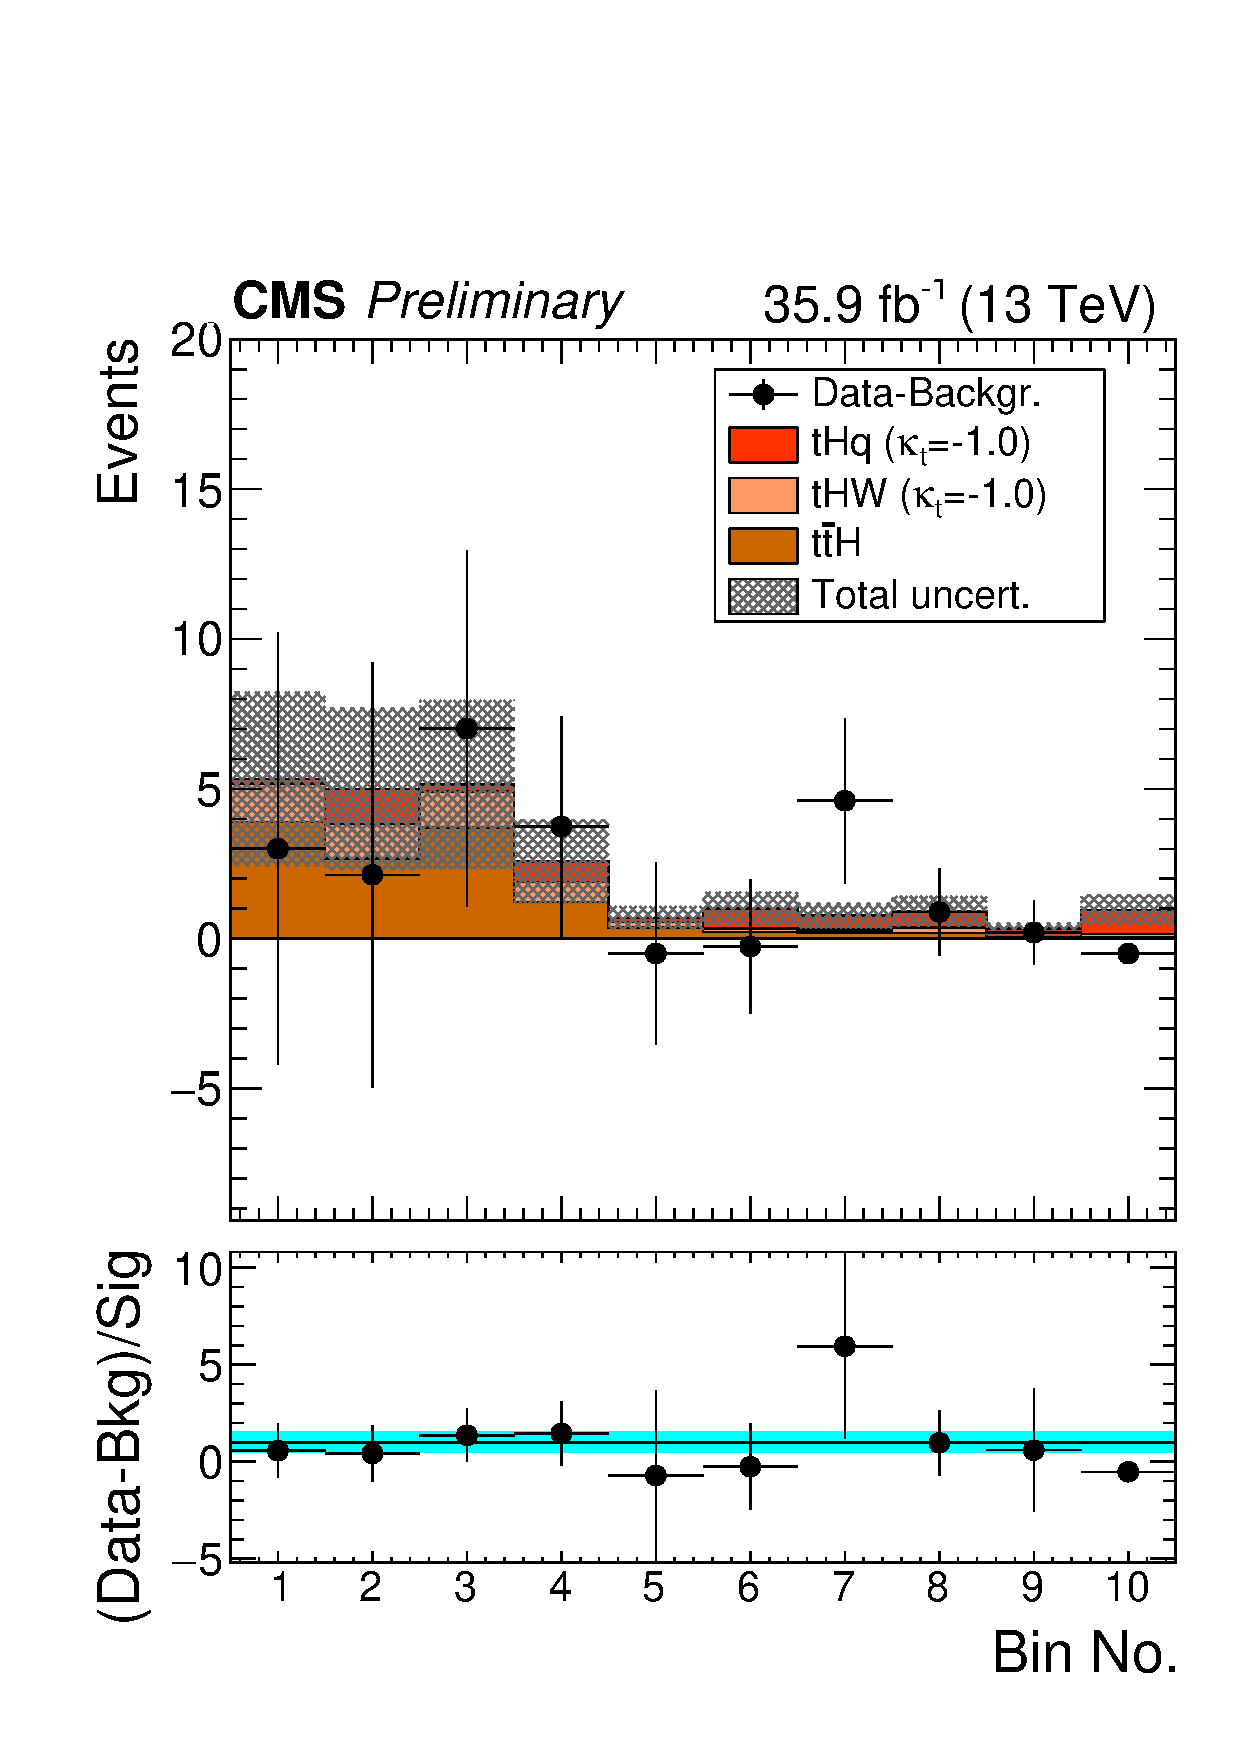
\includegraphics[width=0.32\textwidth]{figures/postfit/bgsub/ITC/tHq_3l_13TeV_fit_s.pdf}
 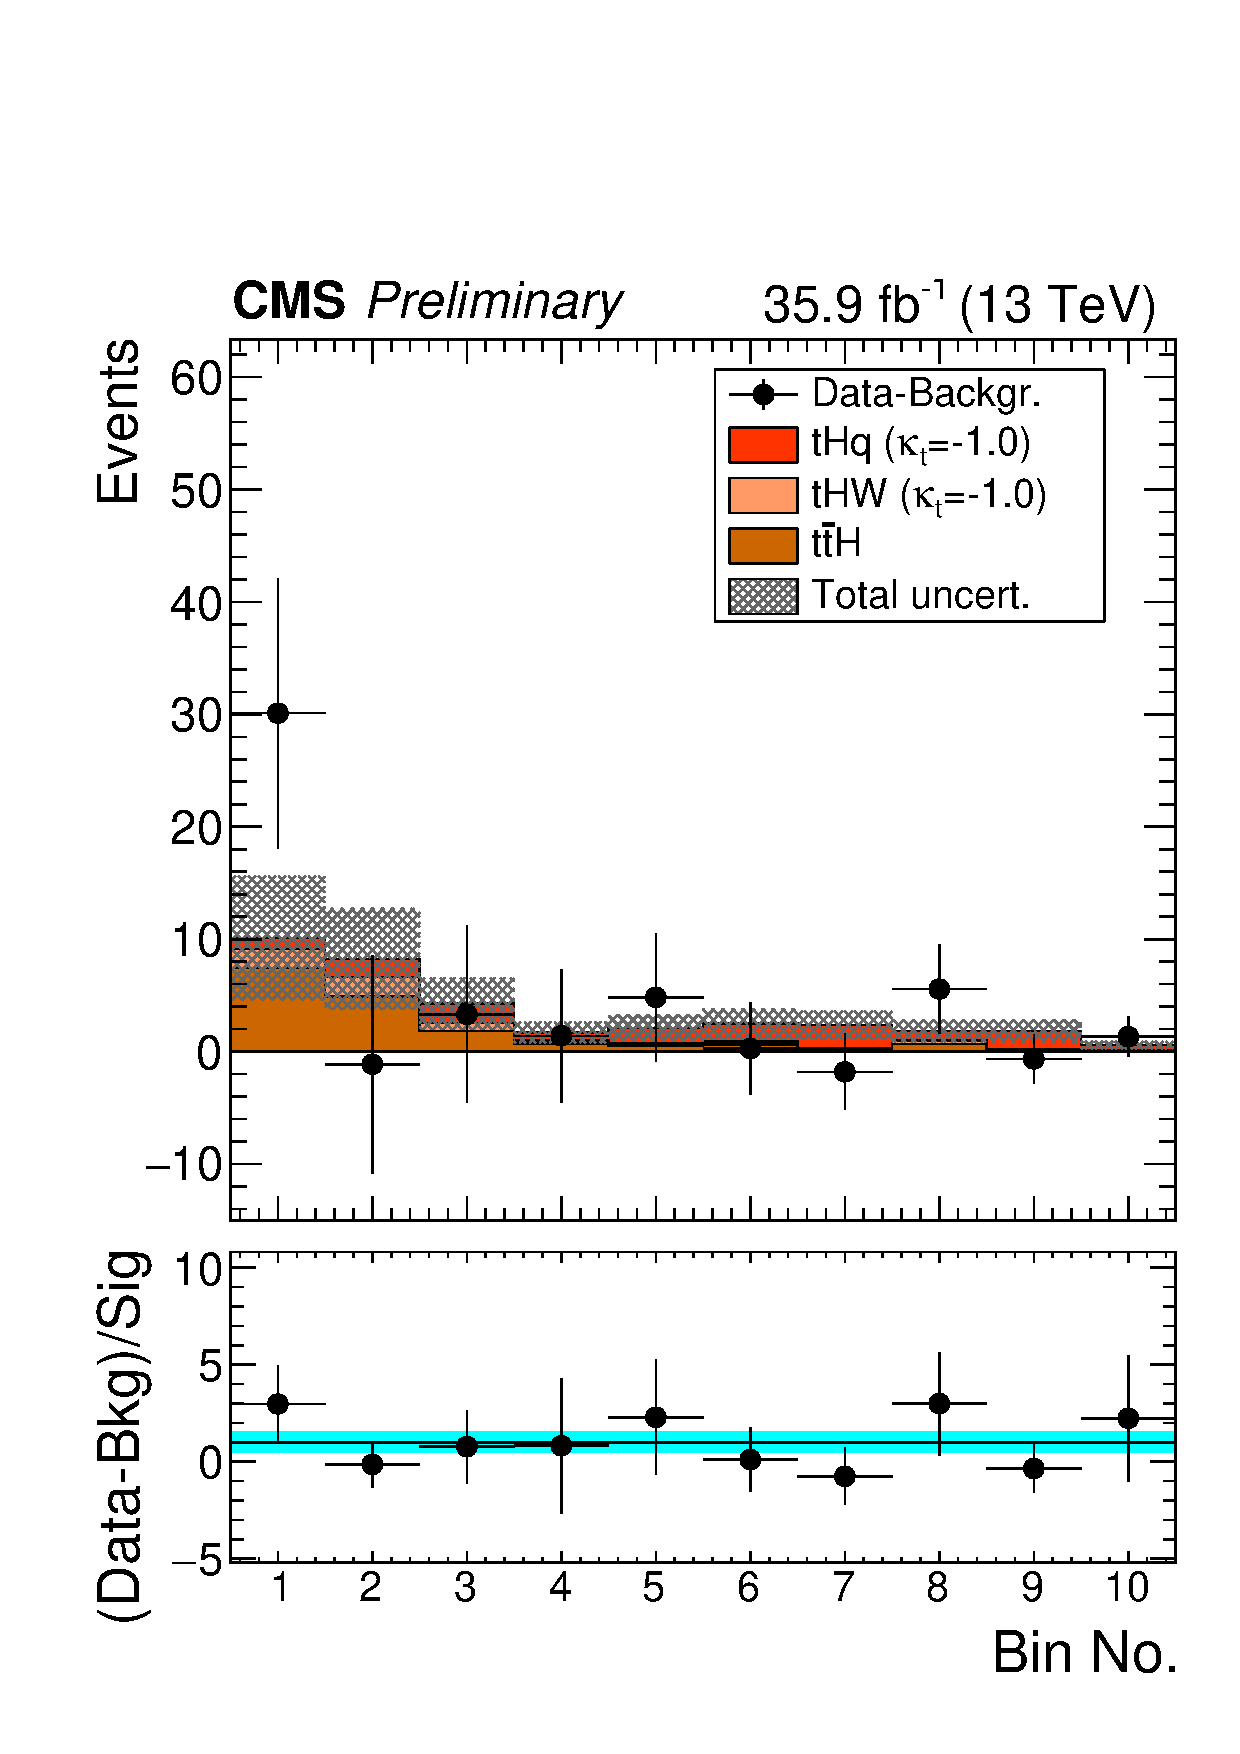
\includegraphics[width=0.32\textwidth]{figures/postfit/bgsub/ITC/tHq_2lss_mm_13TeV_fit_s.pdf}
 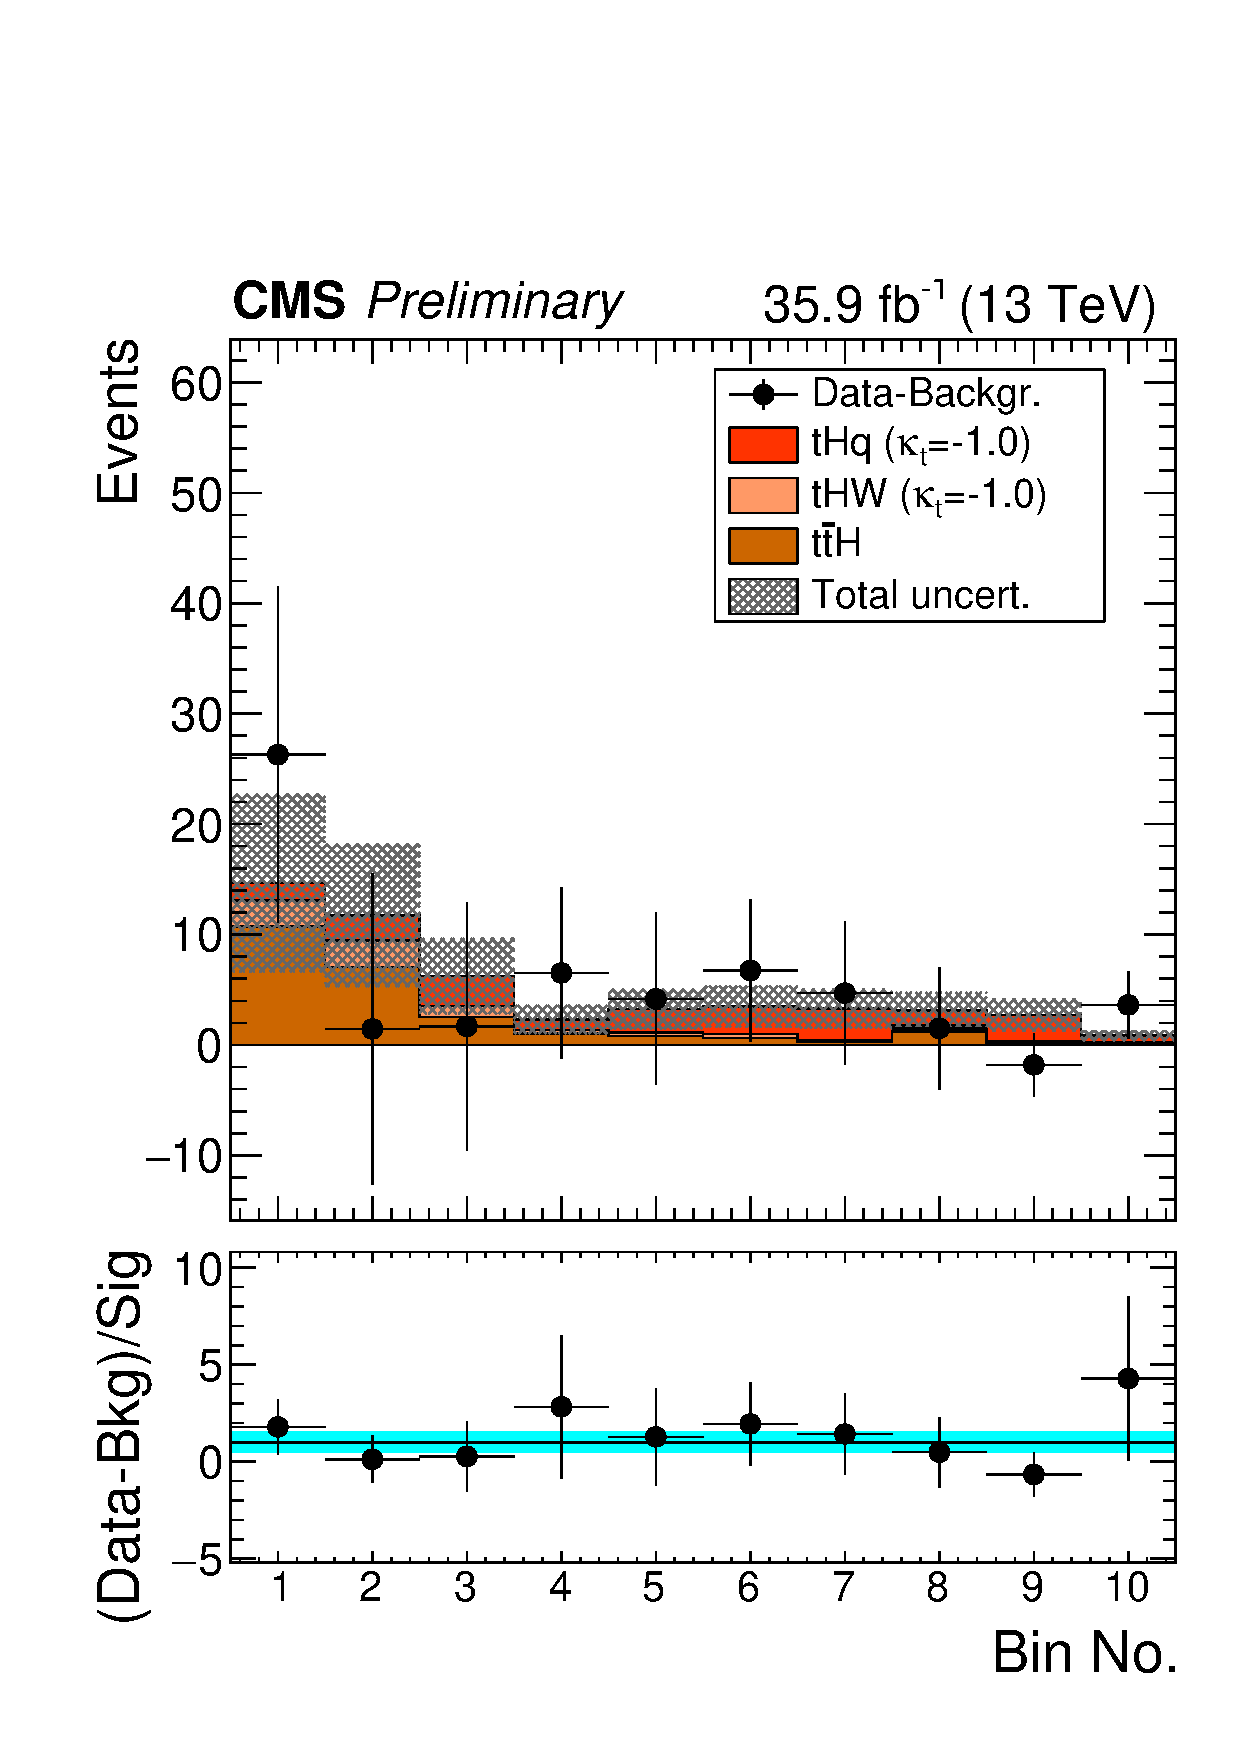
\includegraphics[width=0.32\textwidth]{figures/postfit/bgsub/ITC/tHq_2lss_em_13TeV_fit_s.pdf}
\caption{Background-subtracted pre- (top) and post-fit (bottom) distributions in the final binning used for the signal extraction, for (from left to right) the three lepton channel, the \mumu\ channel, and the \emu\ channel. For a fit in the inverted couplings scenario, as Figs.~\ref{fig:finalbins} and~\ref{fig:postfit}.}
\label{fig:postfit_bgsub_ITC}
\end{figure}

\begin{figure} [!h]
 \centering
 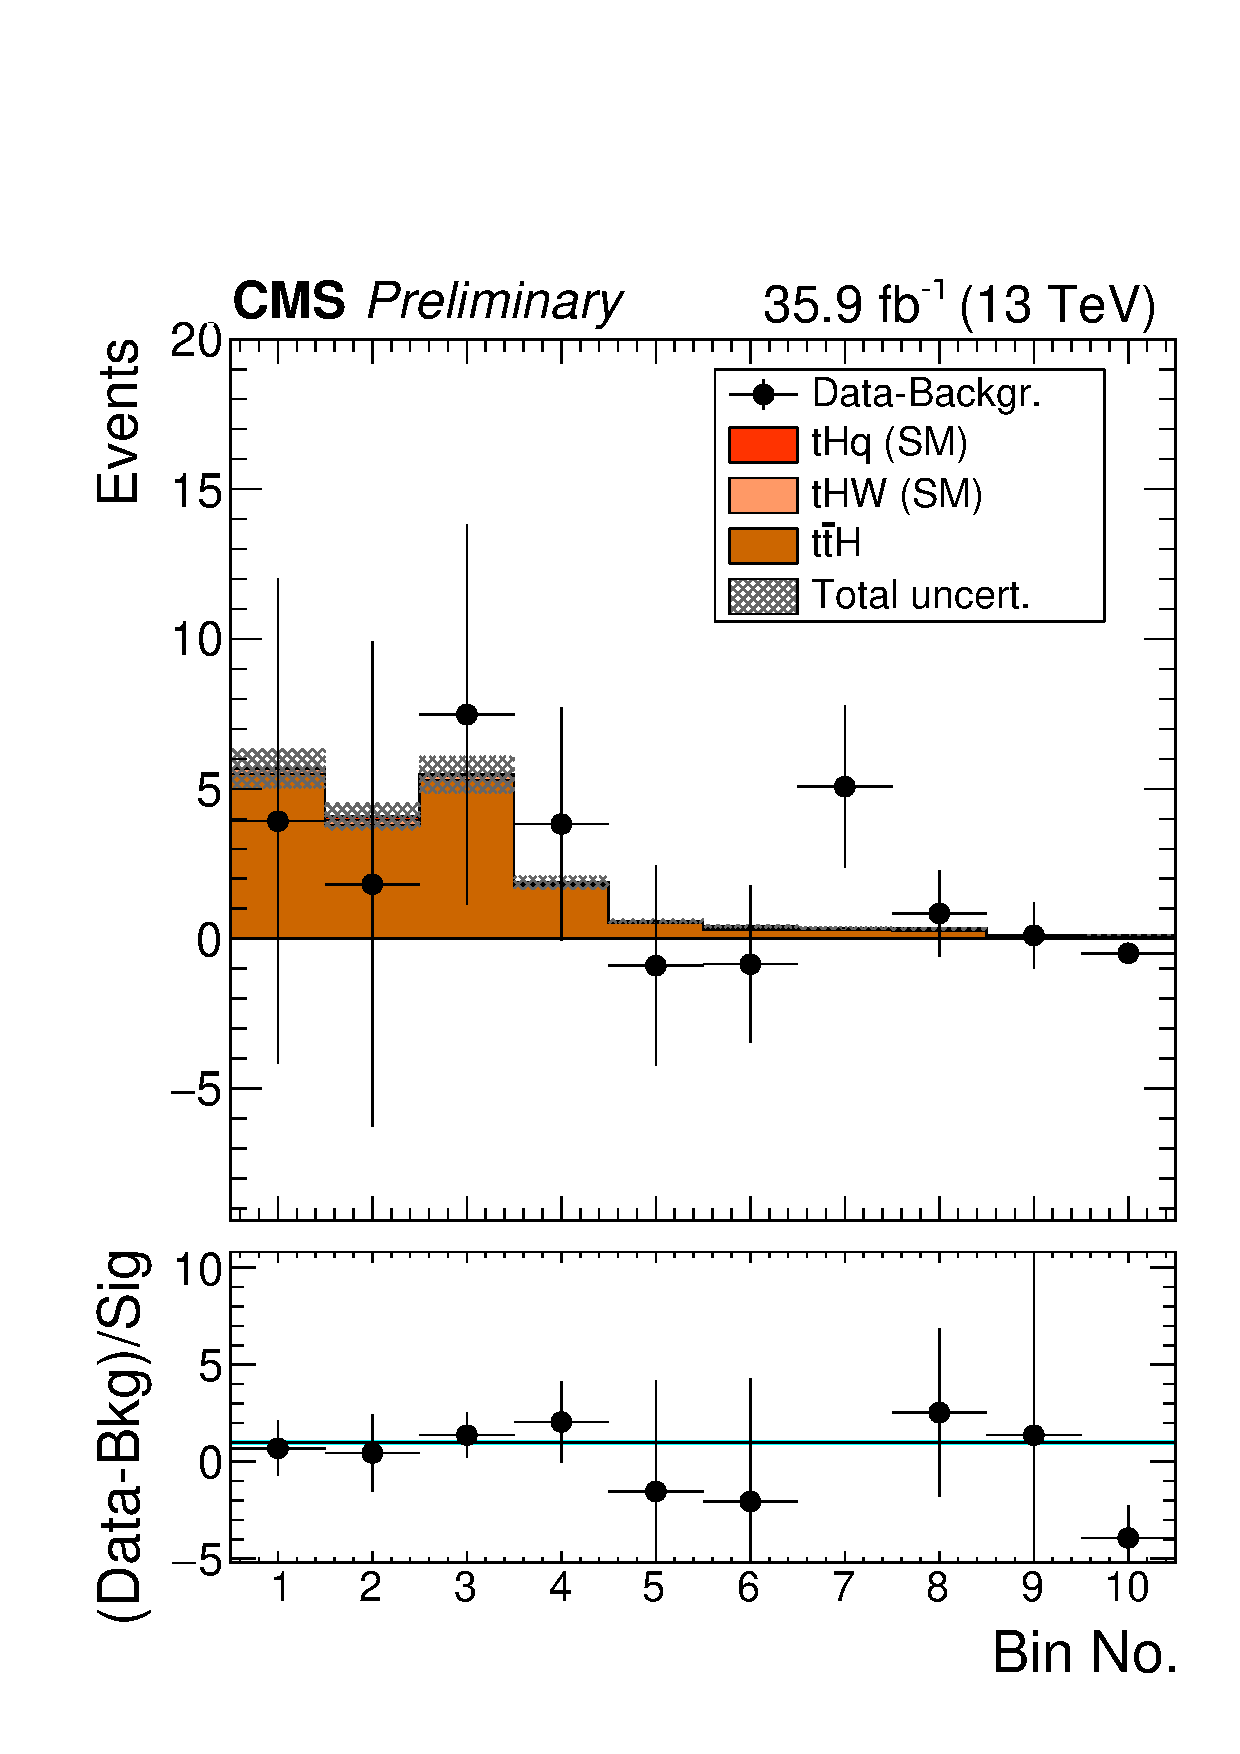
\includegraphics[width=0.32\textwidth]{figures/postfit/bgsub/SM/tHq_3l_13TeV_prefit.pdf}
 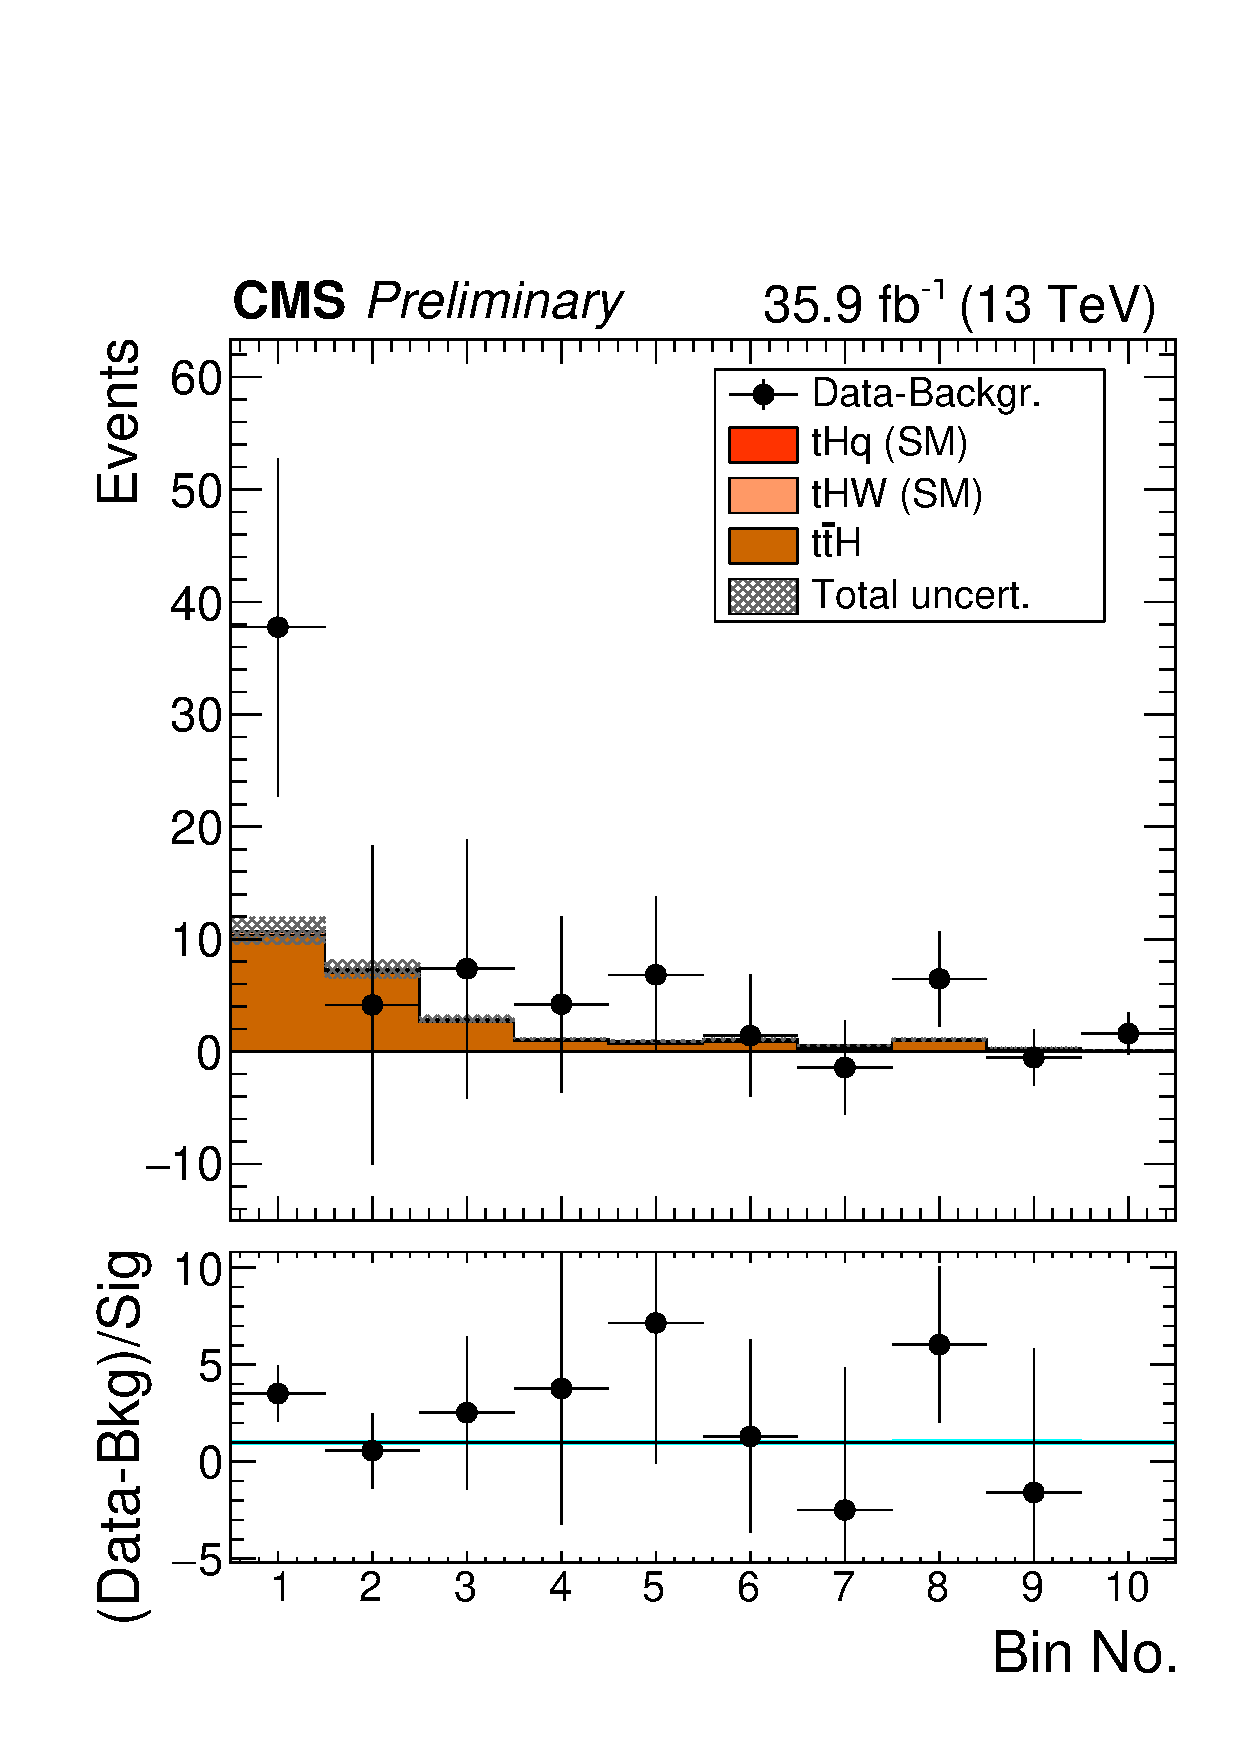
\includegraphics[width=0.32\textwidth]{figures/postfit/bgsub/SM/tHq_2lss_mm_13TeV_prefit.pdf}
 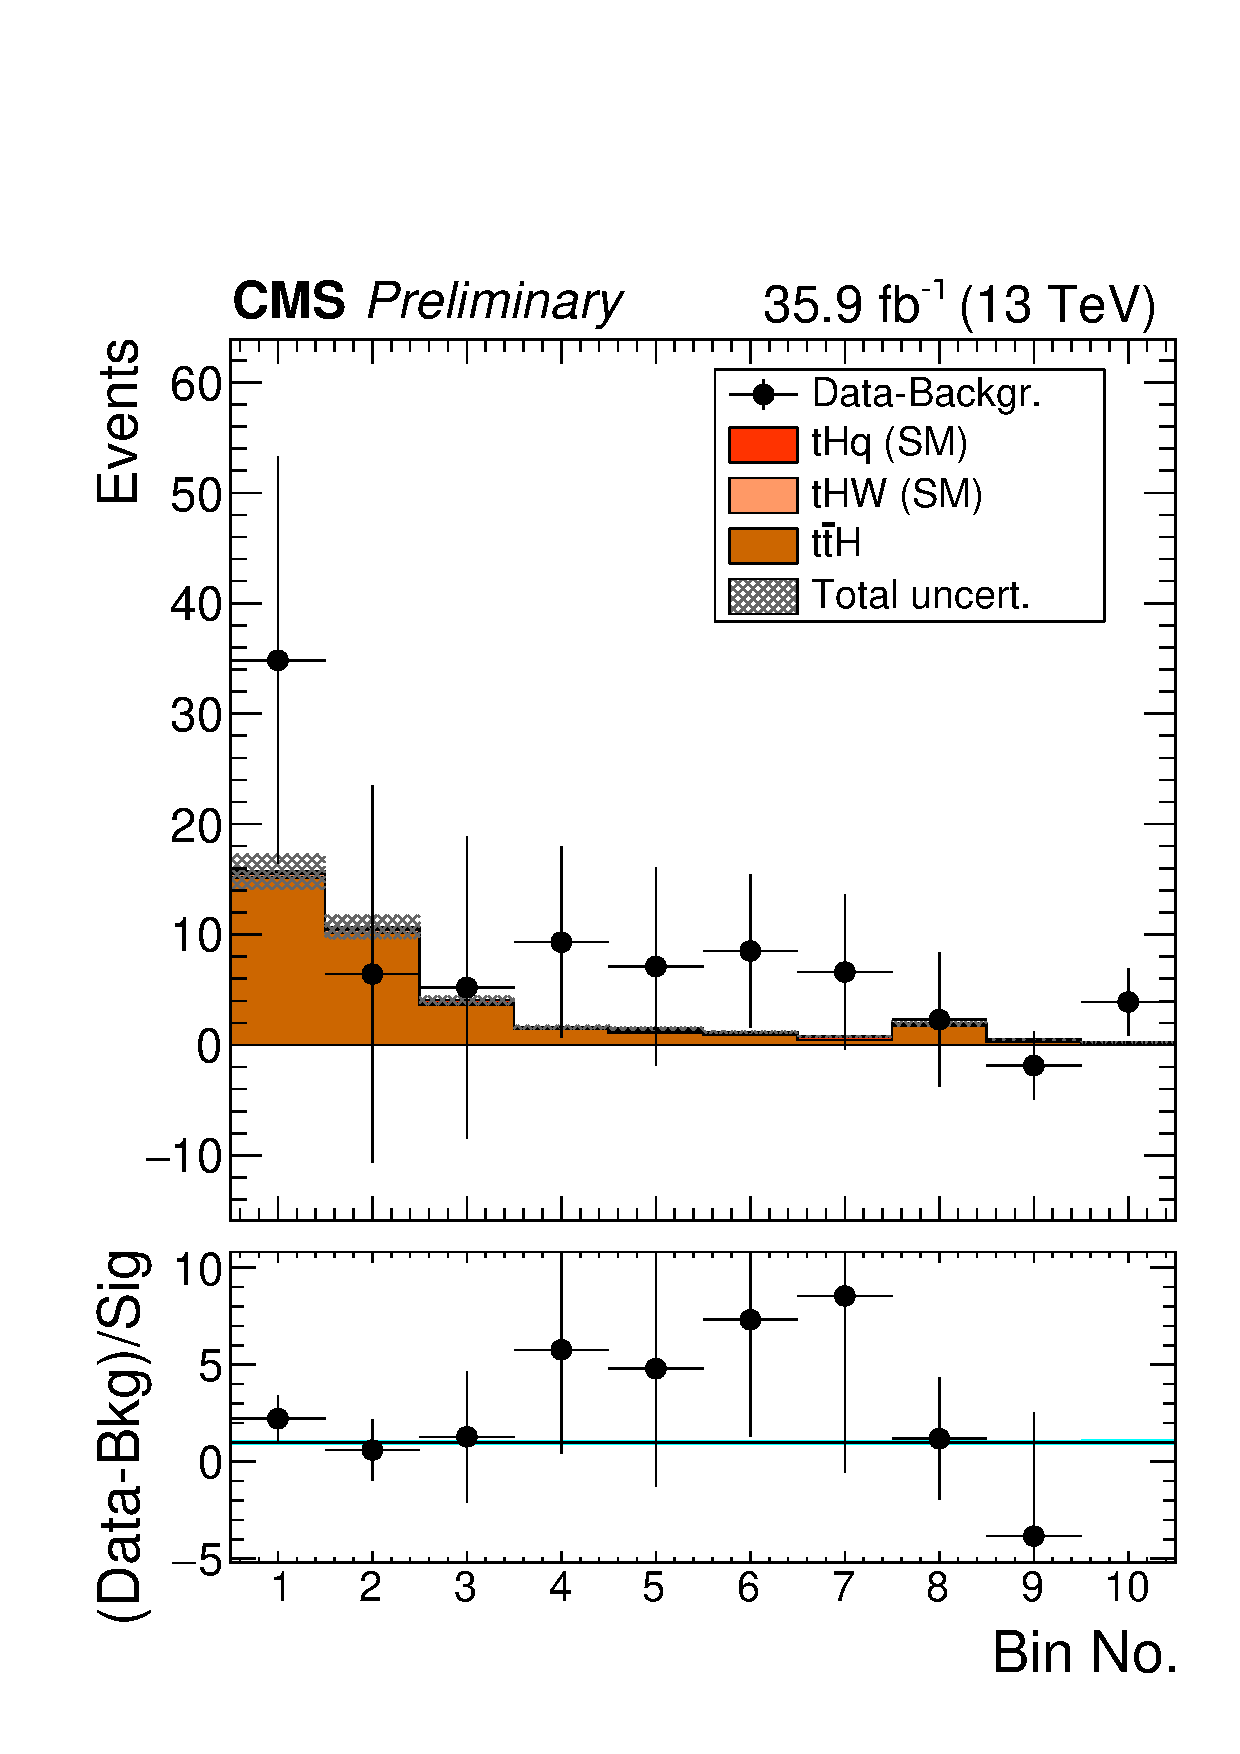
\includegraphics[width=0.32\textwidth]{figures/postfit/bgsub/SM/tHq_2lss_em_13TeV_prefit.pdf} \\
 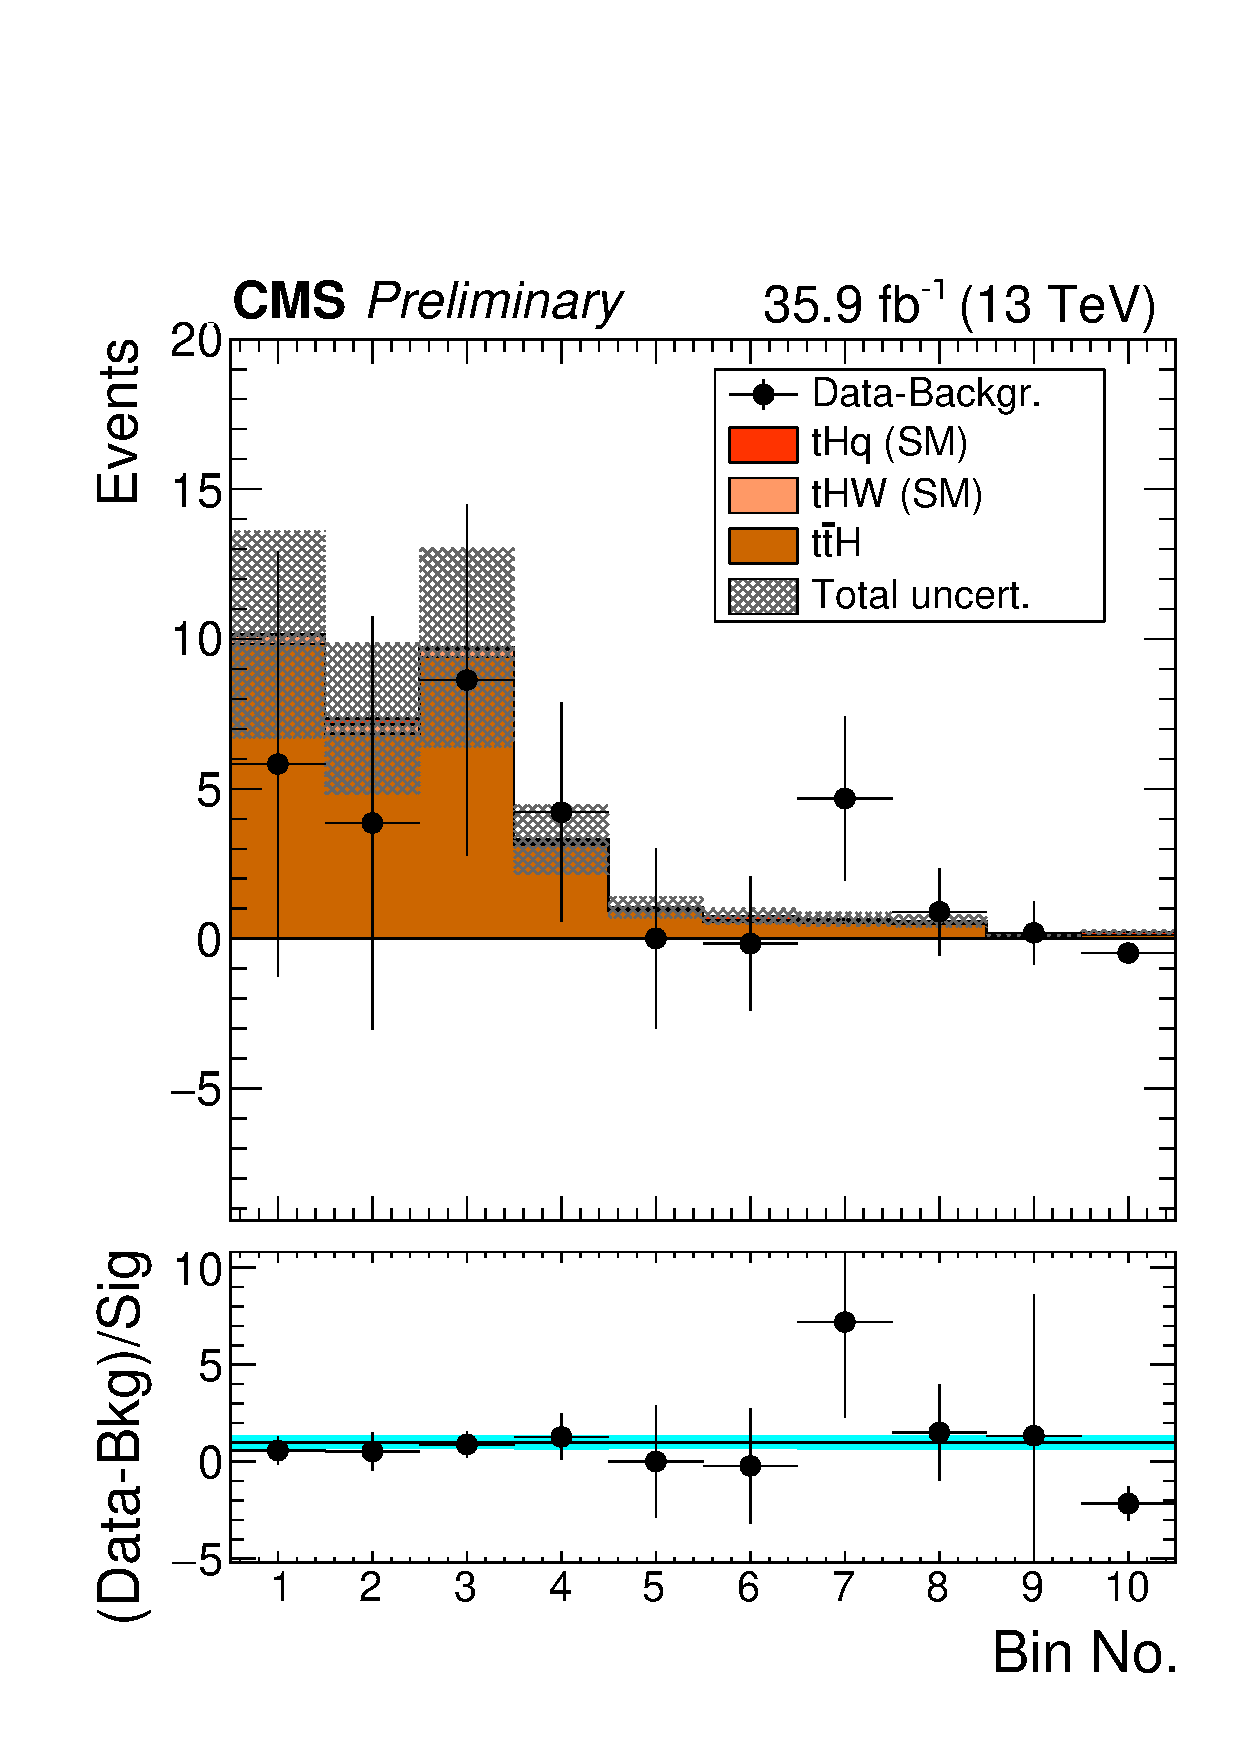
\includegraphics[width=0.32\textwidth]{figures/postfit/bgsub/SM/tHq_3l_13TeV_fit_s.pdf}
 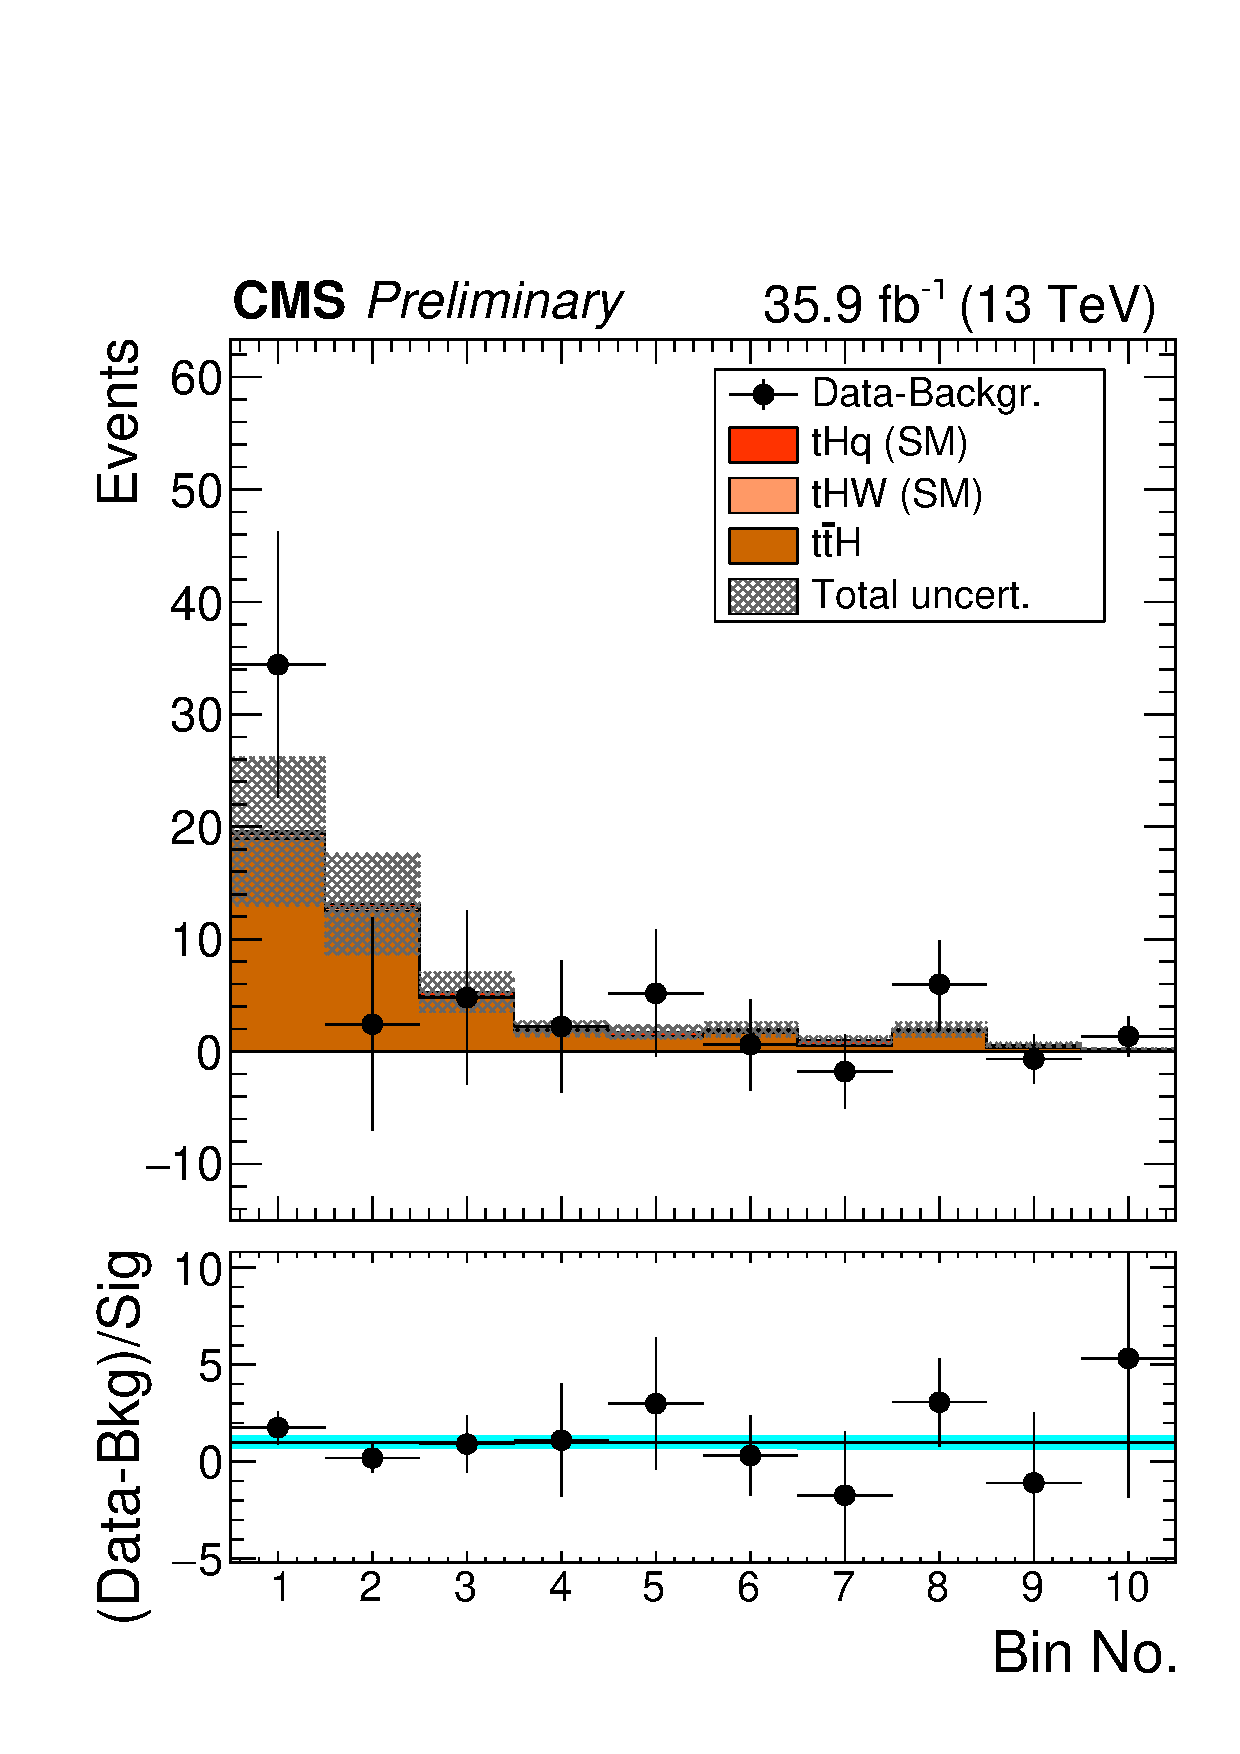
\includegraphics[width=0.32\textwidth]{figures/postfit/bgsub/SM/tHq_2lss_mm_13TeV_fit_s.pdf}
 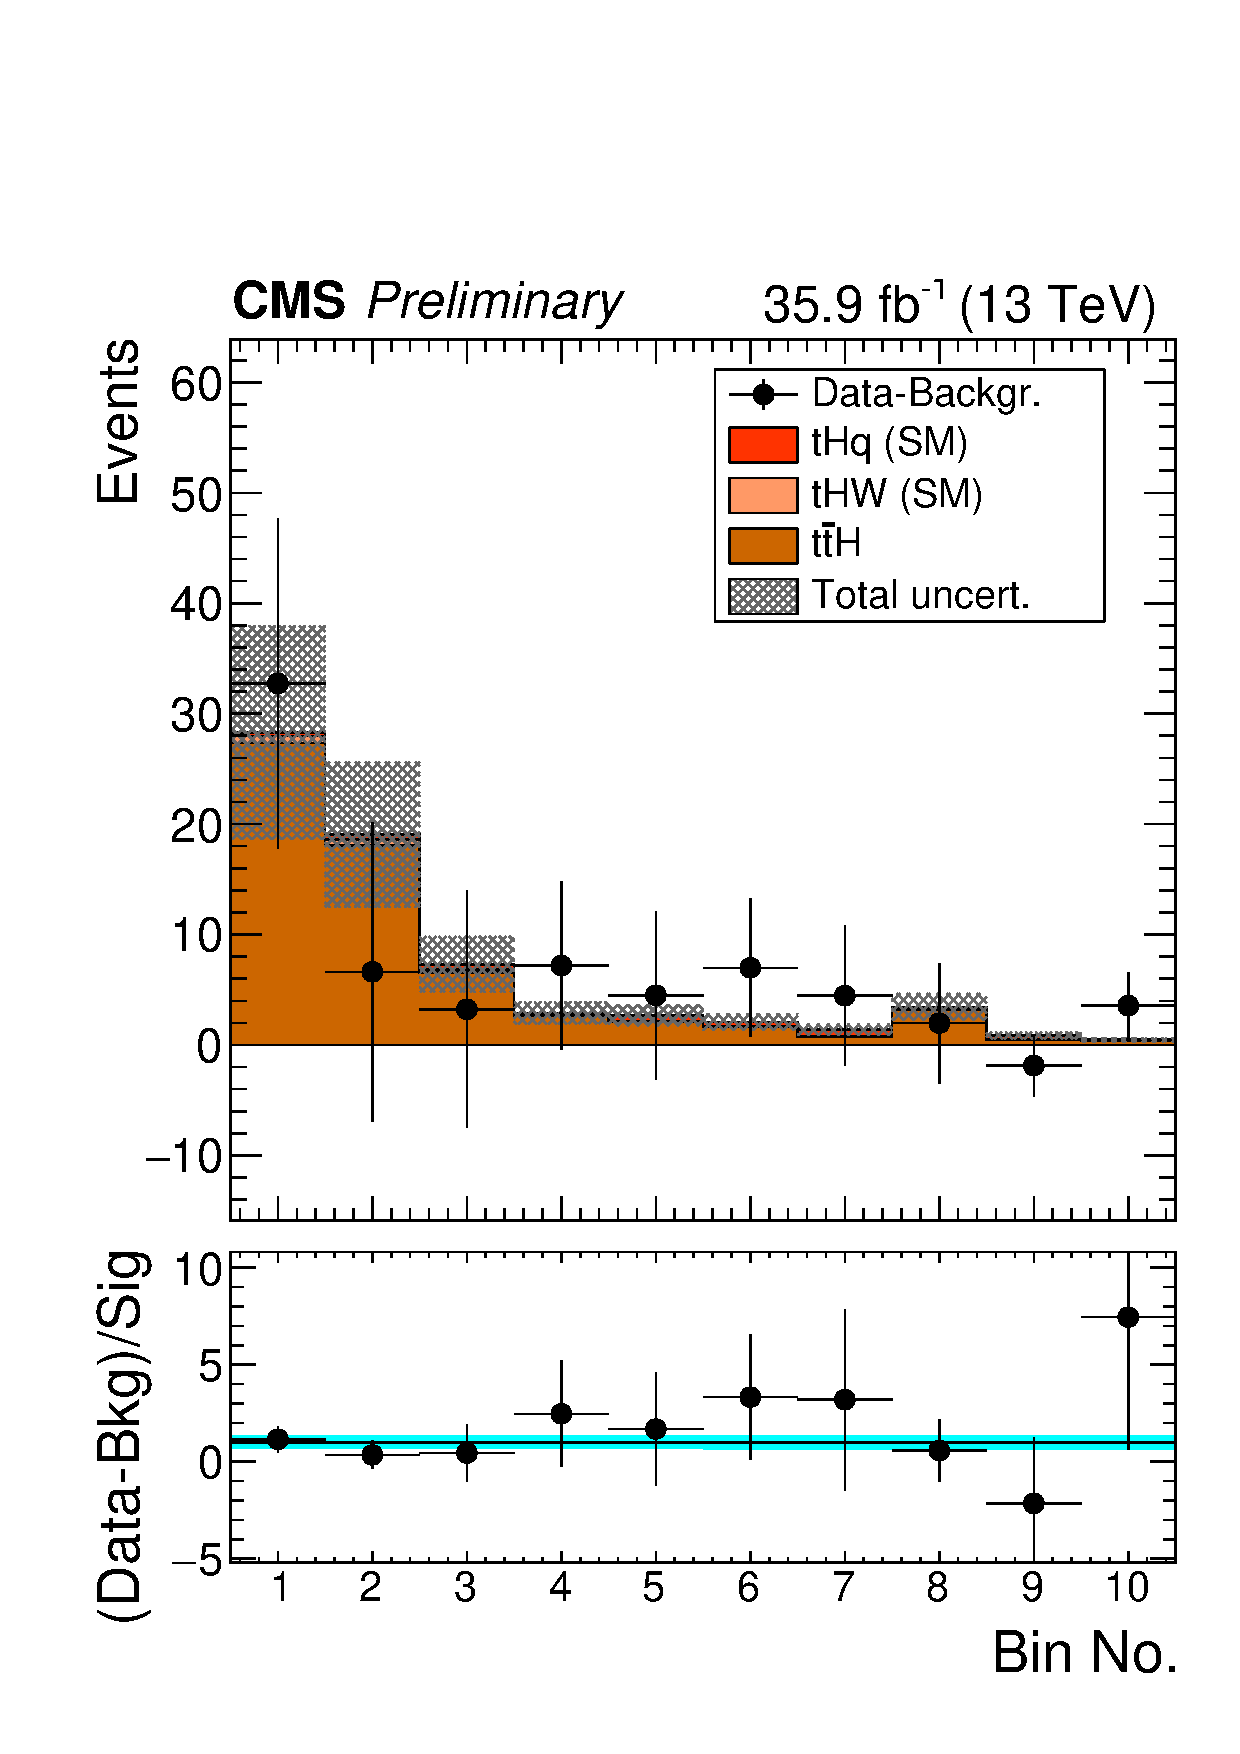
\includegraphics[width=0.32\textwidth]{figures/postfit/bgsub/SM/tHq_2lss_em_13TeV_fit_s.pdf}
\caption{Background-subtracted pre- (top) and post-fit (bottom) distributions in the final binning used for the signal extraction, for (from left to right) the three lepton channel, the \mumu\ channel, and the \emu\ channel. For a fit in the SM-like scenario ($\Ct=\CV=1$).}
\label{fig:postfit_bgsub_SM}
\end{figure}

We calculate asymptotic upper CL$_\text{S}$ limits at 95\% C.L. on the combined production cross section of \tHq, \tHW, and \ttH\ (reported as an upper limit on the cross section times modified branching ratio), for each of the 51 coupling configurations, see Tab.~\ref{tab:limits}.
The limits and best-fit values of the signal cross section (and corresponding signal strength at $\CV=1.0$) for each point are given in Tab.~\ref{tab:xslimits}, and in Tab.~\ref{tab:xslimits_chan} for the two main hypotheses, split by channel.
In the SM point a signal strength of $1.82\,^{+0.34}_{-0.33}\mathrm{(stat.)}\,^{+0.55}_{-0.59}\mathrm{(syst.)}$ (compared to the SM cross section at $\CV=1.0$) is obtained, corresponding to a cross section of $0.33\pm0.12\,\mathrm{pb}$.
The observed significance of the signal, in a background-only hypothesis, is $2.7\,\sigma$, with an a-priori expected significance of $1.5\,\sigma$.
Without considering systematic uncertainties, the significance increases to $6.2\,\sigma$.
A scan of the observed and expected significances for each coupling configuration is shown in Fig.~\ref{fig:significances}.

% The full results are shown in Fig.~\ref{fig:r_limits_cv} for the non-resolved model with fixed $\PH\to\gamma\gamma/\Z\gamma/\Pg\Pg$ branching ratios, and the two scenarios of exactly inverted couplings ($\CV=1.0$,$\Ct=-1.0$) and the standard model are reported in Tab.~\ref{tab:limits}.  %% FIXME
The pulls and impacts of the most important nuisance parameters are shown in Fig.~\ref{fig:impacts}.

\begin{table}[h!]
\centering
\begin{tabular}{llcccccc}
Scenario  & Channel   & Obs. Limit & \multicolumn{5}{c}{Exp. Limit}         \\
           &                                  &     & $-2\sigma$ &$-1\sigma$ & Median        & $+1\sigma$ & $+2\sigma$  \\ \hline
$\CV=1.0$  & \mumu\                           & 2.3          & 0.71 & 0.94 &         1.32  & 1.88 & 2.60 \\
$\Ct=-1.0$ & \emu\                            & 1.9          & 0.65 & 0.87 &         1.21  & 1.71 & 2.32 \\
           % & \ee\                             & 3.3          & 1.05 & 1.41 &         1.98  & 2.80 & 3.86 \\
           & \threel\                         & 1.6          & 0.43 & 0.59 &         0.86  & 1.26 & 1.78 \\
           & Combined ($\mu\mu,3\ell$)        & \textbf{1.6} & 0.40 & 0.54 & \textbf{0.78} & 1.12 & 1.57 \\
           & Combined ($\mu\mu,\Pe\mu,3\ell$) & \textbf{1.4} & 0.37 & 0.50 & \textbf{0.71} & 1.03 & 1.43 \\ \hline
           % & Combined (all channels)          & \textbf{1.6} & 0.37 & 0.51 & \textbf{0.72} & 1.03 & 1.43 \\ \hline
  (SM)     & \mumu\                           & 4.9          & 1.20 & 1.61 &         2.27  & 3.24 & 4.54 \\
$\CV=1.0$  & \emu\                            & 3.3          & 1.10 & 1.48 &         2.07  & 2.95 & 4.06 \\
% $\Ct=1.0$  & \ee\                             & 4.4          & 1.65 & 2.24 &         3.20  & 4.62 & 6.52 \\
$\Ct=1.0$  & \threel\                         & 3.0          & 0.91 & 1.22 &         1.73  & 2.49 & 3.47 \\
           & Combined ($\mu\mu,3\ell$)        & \textbf{3.4} & 0.79 & 1.07 & \textbf{1.51} & 2.17 & 3.01 \\
           & Combined ($\mu\mu,\Pe\mu,3\ell$) & \textbf{3.1} & 0.71 & 0.96 & \textbf{1.36} & 1.94 & 2.70 \\ \hline
           % & Combined (all channels)          & \textbf{3.1} & 0.71 & 0.95 & \textbf{1.34} & 1.92 & 2.65 \\ \hline
\end{tabular}
\caption{Expected and observed CL$_\text{S}$ limits (at 95\% C.L.) on the signal strength of combined $\tH+\ttH$ production in each channel, and for different combinations thereof, for a scenario with inverted couplings ($\CV=1.0$, $\Ct=-1.0$, top section), and for the standard model ($\CV=\Ct=1.0$, bottom section). Numbers are for 35.9\fbinv.}
\label{tab:limits}
\end{table}

\begin{table}[h!]
  \begin{center}
    \begin{tabular}{llcccc} \hline 
      Scenario  & Channel  & Obs. Limit    & \multicolumn{3}{c}{Exp. Limit (pb)}         \\
                &          & (pb)          & Median        & $\pm1\sigma$ & $\pm2\sigma$ \\ \hline \hline
   $\Ct/\CV=-1$ & \mumu\   & 1.00          &         0.58  & [0.42, 0.83] & [0.31, 1.15] \\
                & \emu\    & 0.84          &         0.54  & [0.39, 0.76] & [0.29, 1.03] \\
                & \threel\ & 0.70          &         0.38  & [0.26, 0.56] & [0.19, 0.79] \\ 
                & Combined & \textbf{0.64} & \textbf{0.32} & [0.22, 0.46] & [0.16, 0.64] \\ \hline
    $\Ct/\CV=1$ & \mumu\   & 0.87          &         0.41  & [0.29, 0.58] & [0.22, 0.82] \\
    (SM-like)   & \emu\    & 0.59          &         0.37  & [0.26, 0.53] & [0.20, 0.73] \\
                & \threel\ & 0.54          &         0.31  & [0.22, 0.43] & [0.16, 0.62] \\
                & Combined & \textbf{0.56} & \textbf{0.24} & [0.17, 0.35] & [0.13, 0.49] \\ \hline
    \end{tabular}
    \caption{Expected and observed 95\% C.L. upper limits on the $\tH+\ttH$ production cross section times $\PH\to\W\W^*+\tautau+\Z\Z^*$ branching ratio for a scenario of inverted couplings ($\Ct/\CV=-1.0$, top rows) and for a standard-model-like signal ($\Ct/\CV=1.0$, bottom rows), in pb. The expected limit is calculated on a background-only Asimov dataset and quoted with $\pm$1$\sigma$ and $\pm$2$\sigma$ probability ranges.
    \label{tab:xslimits_chan}}
  \end{center}
\end{table}


\begin{table}[h!]
\centering
\begin{tabular}{rr|ccc|cc}
$f_t$  & \Ct/\CV\ & Exp.\ lim. & SM exp. & Obs.\ lim. & Best fit $\sigma$ [pb] & Best fit $r$ \\ \hline
-0.973 & -6.000 & $0.328~_{-0.090}^{+0.136}$ & $0.507~_{-0.158}^{+0.206}$ & 0.603 & $0.305~_{-0.169}^{+0.155}$ & $0.013~_{-0.007}^{+0.007}$ \\
-0.941 & -4.000 & $0.335~_{-0.098}^{+0.137}$ & $0.509~_{-0.166}^{+0.215}$ & 0.627 & $0.322~_{-0.174}^{+0.157}$ & $0.036~_{-0.020}^{+0.018}$ \\
-0.900 & -3.000 & $0.335~_{-0.096}^{+0.138}$ & $0.510~_{-0.172}^{+0.215}$ & 0.639 & $0.334~_{-0.173}^{+0.160}$ & $0.075~_{-0.039}^{+0.036}$ \\
-0.862 & -2.500 & $0.334~_{-0.097}^{+0.139}$ & $0.505~_{-0.173}^{+0.217}$ & 0.649 & $0.341~_{-0.174}^{+0.160}$ & $0.119~_{-0.061}^{+0.056}$ \\
-0.800 & -2.000 & $0.330~_{-0.095}^{+0.141}$ & $0.500~_{-0.176}^{+0.212}$ & 0.656 & $0.345~_{-0.176}^{+0.165}$ & $0.202~_{-0.103}^{+0.097}$ \\
-0.692 & -1.500 & $0.325~_{-0.095}^{+0.139}$ & $0.485~_{-0.172}^{+0.209}$ & 0.660 & $0.340~_{-0.176}^{+0.164}$ & $0.369~_{-0.191}^{+0.178}$ \\
-0.640 & -1.333 & $0.325~_{-0.097}^{+0.139}$ & $0.482~_{-0.173}^{+0.210}$ & 0.659 & $0.334~_{-0.174}^{+0.169}$ & $0.456~_{-0.238}^{+0.231}$ \\
-0.610 & -1.250 & $0.321~_{-0.095}^{+0.140}$ & $0.474~_{-0.169}^{+0.210}$ & 0.653 & $0.328~_{-0.177}^{+0.164}$ & $0.505~_{-0.272}^{+0.252}$ \\
-0.500 & -1.000 & $0.315~_{-0.093}^{+0.142}$ & $0.450~_{-0.160}^{+0.213}$ & 0.638 & $0.304~_{-0.176}^{+0.175}$ & $0.685~_{-0.396}^{+0.395}$ \\
-0.410 & -0.833 & $0.312~_{-0.095}^{+0.138}$ & $0.424~_{-0.147}^{+0.210}$ & 0.615 & $0.276~_{-0.177}^{+0.168}$ & $0.819~_{-0.526}^{+0.498}$ \\
-0.360 & -0.750 & $0.307~_{-0.093}^{+0.138}$ & $0.409~_{-0.136}^{+0.200}$ & 0.593 & $0.256~_{-0.176}^{+0.170}$ & $0.874~_{-0.601}^{+0.581}$ \\
-0.308 & -0.667 & $0.301~_{-0.092}^{+0.138}$ & $0.384~_{-0.124}^{+0.198}$ & 0.566 & $0.231~_{-0.174}^{+0.165}$ & $0.915~_{-0.689}^{+0.655}$ \\
-0.200 & -0.500 & $0.292~_{-0.090}^{+0.136}$ & $0.345~_{-0.109}^{+0.181}$ & 0.497 & $0.166~_{-0.162}^{+0.163}$ & $0.895~_{-0.871}^{+0.879}$ \\
-0.100 & -0.333 & $0.278~_{-0.086}^{+0.132}$ & $0.303~_{-0.092}^{+0.156}$ & 0.409 & $0.092~_{-0.092}^{+0.157}$ & $0.679~_{-0.679}^{+1.159}$ \\
-0.059 & -0.250 & $0.268~_{-0.083}^{+0.129}$ & $0.283~_{-0.085}^{+0.152}$ & 0.365 & $0.059~_{-0.059}^{+0.148}$ & $0.515~_{-0.515}^{+1.285}$ \\
-0.027 & -0.167 & $0.260~_{-0.081}^{+0.125}$ & $0.266~_{-0.077}^{+0.135}$ & 0.328 & $0.029~_{-0.029}^{+0.142}$ & $0.297~_{-0.297}^{+1.434}$ \\
 0.000 &  0.000 & $0.254~_{-0.079}^{+0.123}$ & $0.252~_{-0.073}^{+0.123}$ & 0.294 & $0.000~_{-0.000}^{+0.132}$ & $0.002~_{-0.002}^{+1.776}$ \\
 0.027 &  0.167 & $0.275~_{-0.086}^{+0.132}$ & $0.284~_{-0.084}^{+0.148}$ & 0.357 & $0.040~_{-0.040}^{+0.154}$ & $0.650~_{-0.650}^{+2.514}$ \\
 0.059 &  0.250 & $0.297~_{-0.093}^{+0.141}$ & $0.329~_{-0.099}^{+0.171}$ & 0.458 & $0.119~_{-0.119}^{+0.183}$ & $2.015~_{-2.015}^{+3.098}$ \\
 0.100 &  0.333 & $0.322~_{-0.099}^{+0.148}$ & $0.405~_{-0.135}^{+0.220}$ & 0.611 & $0.246~_{-0.184}^{+0.166}$ & $4.147~_{-3.103}^{+2.802}$ \\
 0.200 &  0.500 & $0.324~_{-0.096}^{+0.141}$ & $0.505~_{-0.181}^{+0.212}$ & 0.730 & $0.413~_{-0.177}^{+0.150}$ & $5.982~_{-2.559}^{+2.174}$ \\
 0.308 &  0.667 & $0.281~_{-0.082}^{+0.122}$ & $0.462~_{-0.159}^{+0.172}$ & 0.651 & $0.382~_{-0.144}^{+0.136}$ & $4.186~_{-1.574}^{+1.492}$ \\
 0.360 &  0.750 & $0.268~_{-0.079}^{+0.116}$ & $0.442~_{-0.154}^{+0.160}$ & 0.620 & $0.364~_{-0.135}^{+0.130}$ & $3.392~_{-1.253}^{+1.214}$ \\
 0.410 &  0.833 & $0.258~_{-0.075}^{+0.112}$ & $0.427~_{-0.147}^{+0.162}$ & 0.599 & $0.351~_{-0.130}^{+0.127}$ & $2.754~_{-1.022}^{+0.999}$ \\
 0.500 &  1.000 & $0.244~_{-0.072}^{+0.105}$ & $0.401~_{-0.137}^{+0.154}$ & 0.562 & $0.328~_{-0.121}^{+0.118}$ & $1.821~_{-0.671}^{+0.657}$ \\
 0.610 &  1.250 & $0.240~_{-0.070}^{+0.104}$ & $0.394~_{-0.133}^{+0.154}$ & 0.545 & $0.315~_{-0.119}^{+0.118}$ & $1.072~_{-0.403}^{+0.399}$ \\
 0.640 &  1.333 & $0.242~_{-0.071}^{+0.105}$ & $0.398~_{-0.136}^{+0.156}$ & 0.547 & $0.316~_{-0.121}^{+0.122}$ & $0.921~_{-0.352}^{+0.354}$ \\
 0.692 &  1.500 & $0.244~_{-0.071}^{+0.106}$ & $0.401~_{-0.136}^{+0.159}$ & 0.543 & $0.312~_{-0.120}^{+0.120}$ & $0.678~_{-0.261}^{+0.262}$ \\
 0.800 &  2.000 & $0.256~_{-0.075}^{+0.109}$ & $0.416~_{-0.138}^{+0.169}$ & 0.552 & $0.311~_{-0.127}^{+0.121}$ & $0.317~_{-0.129}^{+0.123}$ \\
 0.862 &  2.500 & $0.268~_{-0.078}^{+0.114}$ & $0.433~_{-0.142}^{+0.169}$ & 0.558 & $0.310~_{-0.130}^{+0.127}$ & $0.170~_{-0.072}^{+0.070}$ \\
 0.900 &  3.000 & $0.276~_{-0.080}^{+0.118}$ & $0.442~_{-0.144}^{+0.177}$ & 0.563 & $0.308~_{-0.134}^{+0.128}$ & $0.102~_{-0.044}^{+0.042}$ \\
 0.941 &  4.000 & $0.290~_{-0.084}^{+0.122}$ & $0.459~_{-0.149}^{+0.184}$ & 0.566 & $0.304~_{-0.140}^{+0.134}$ & $0.046~_{-0.021}^{+0.020}$ \\
 0.973 &  6.000 & $0.306~_{-0.081}^{+0.122}$ & $0.474~_{-0.150}^{+0.192}$ & 0.571 & $0.300~_{-0.150}^{+0.131}$ & $0.016~_{-0.008}^{+0.007}$ \\
 \hline
\end{tabular}
\caption{Expected (for background only, and for a SM-like Higgs signal) and observed 95\% C.L. upper limits (in pb), and best fit signal strength $r$ and corresponding best fit cross section for the combined $\tH+\ttH$ cross section times modified branching ratio for the combination of all three channels, for different values of $\Ct/\CV$ or the equivalent $\ft$ numbers.}
\label{tab:xslimits}
\end{table}

\begin{table}[h!]
\centering
\begin{tabular}{lr}
 \hline
  \threel\  & $r=1.44 {}_{-0.84} {}^{+0.91}$ \\
  \emu\     & $r=1.42 {}_{-1.03} {}^{+1.06}$ \\
  \mumu\    & $r=2.75 {}_{-1.11} {}^{+1.22}$ \\
  Combined  & $r=1.82 {}_{-0.69} {}^{+0.76}$ \\ 
  Expected  & $r=1.00 {}_{-0.65} {}^{+0.70}$ \\ 
 \hline
\end{tabular}
\caption{Best-fit signal strengths for a SM-like Higgs signal for the individual channels.}
\label{tab:sigstrengths}
\end{table}


\begin{figure} [!h]
 \centering
 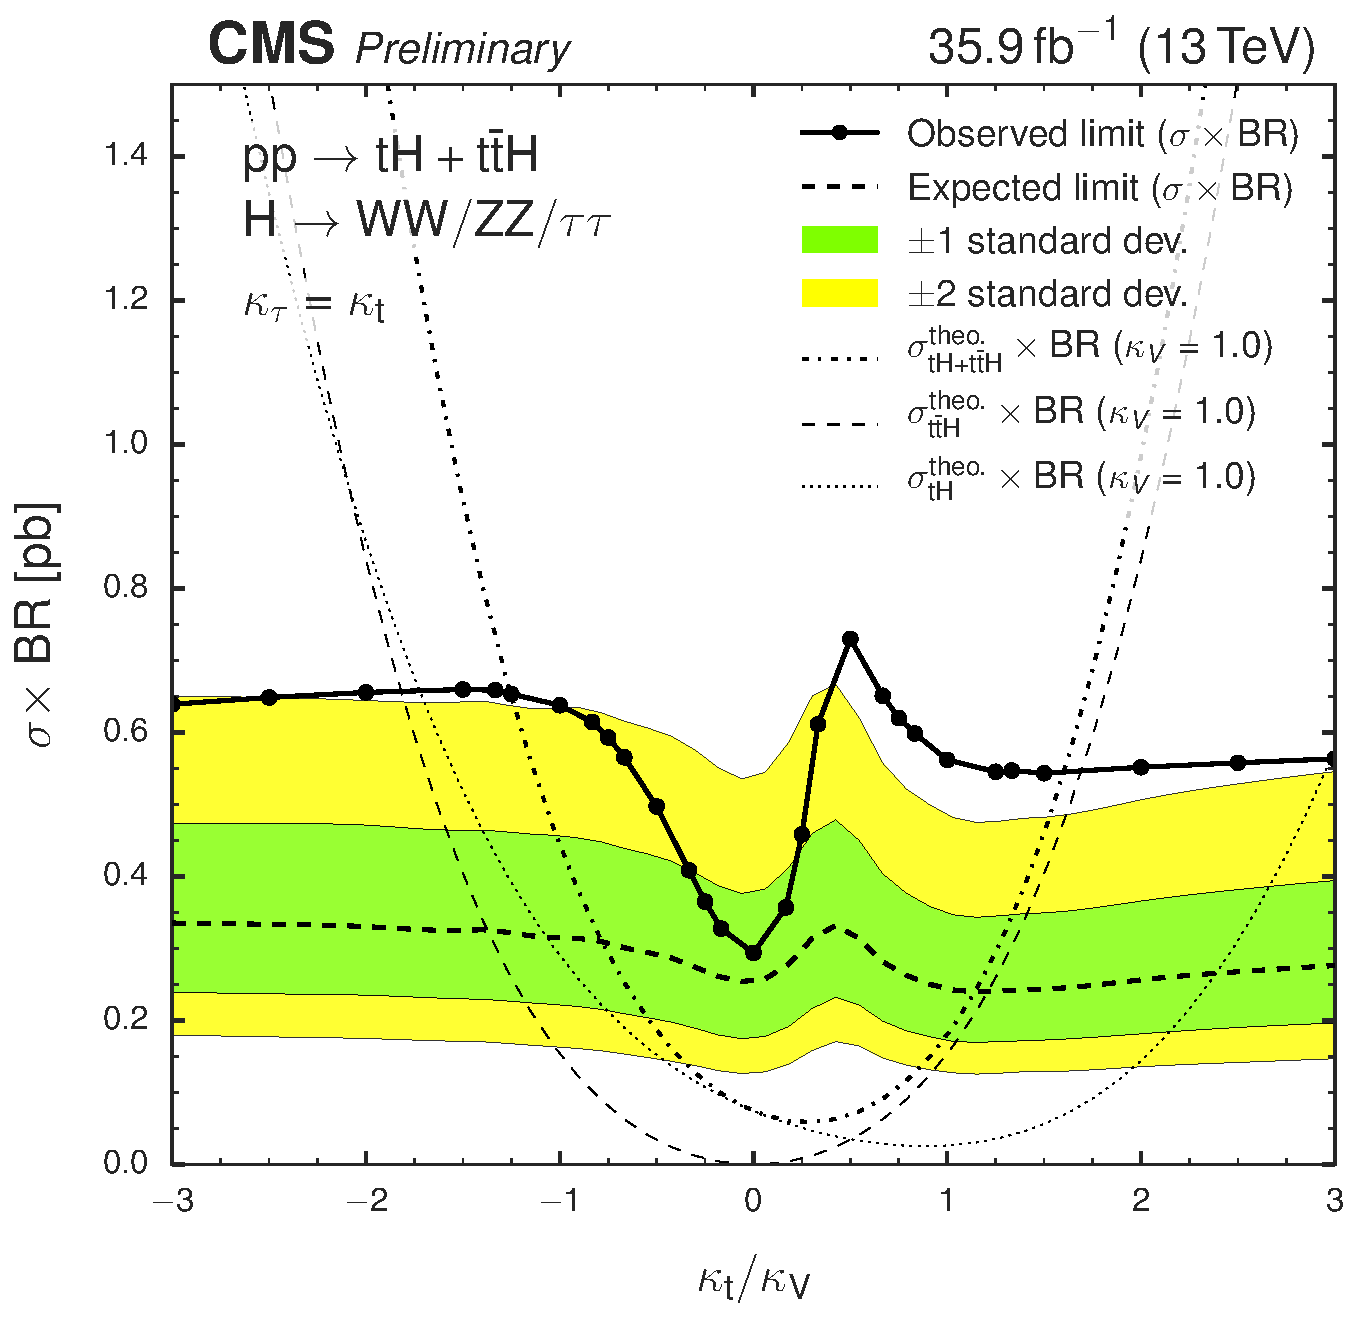
\includegraphics[width=0.48\textwidth]{figures/limits/xs_limits_K6.pdf}
 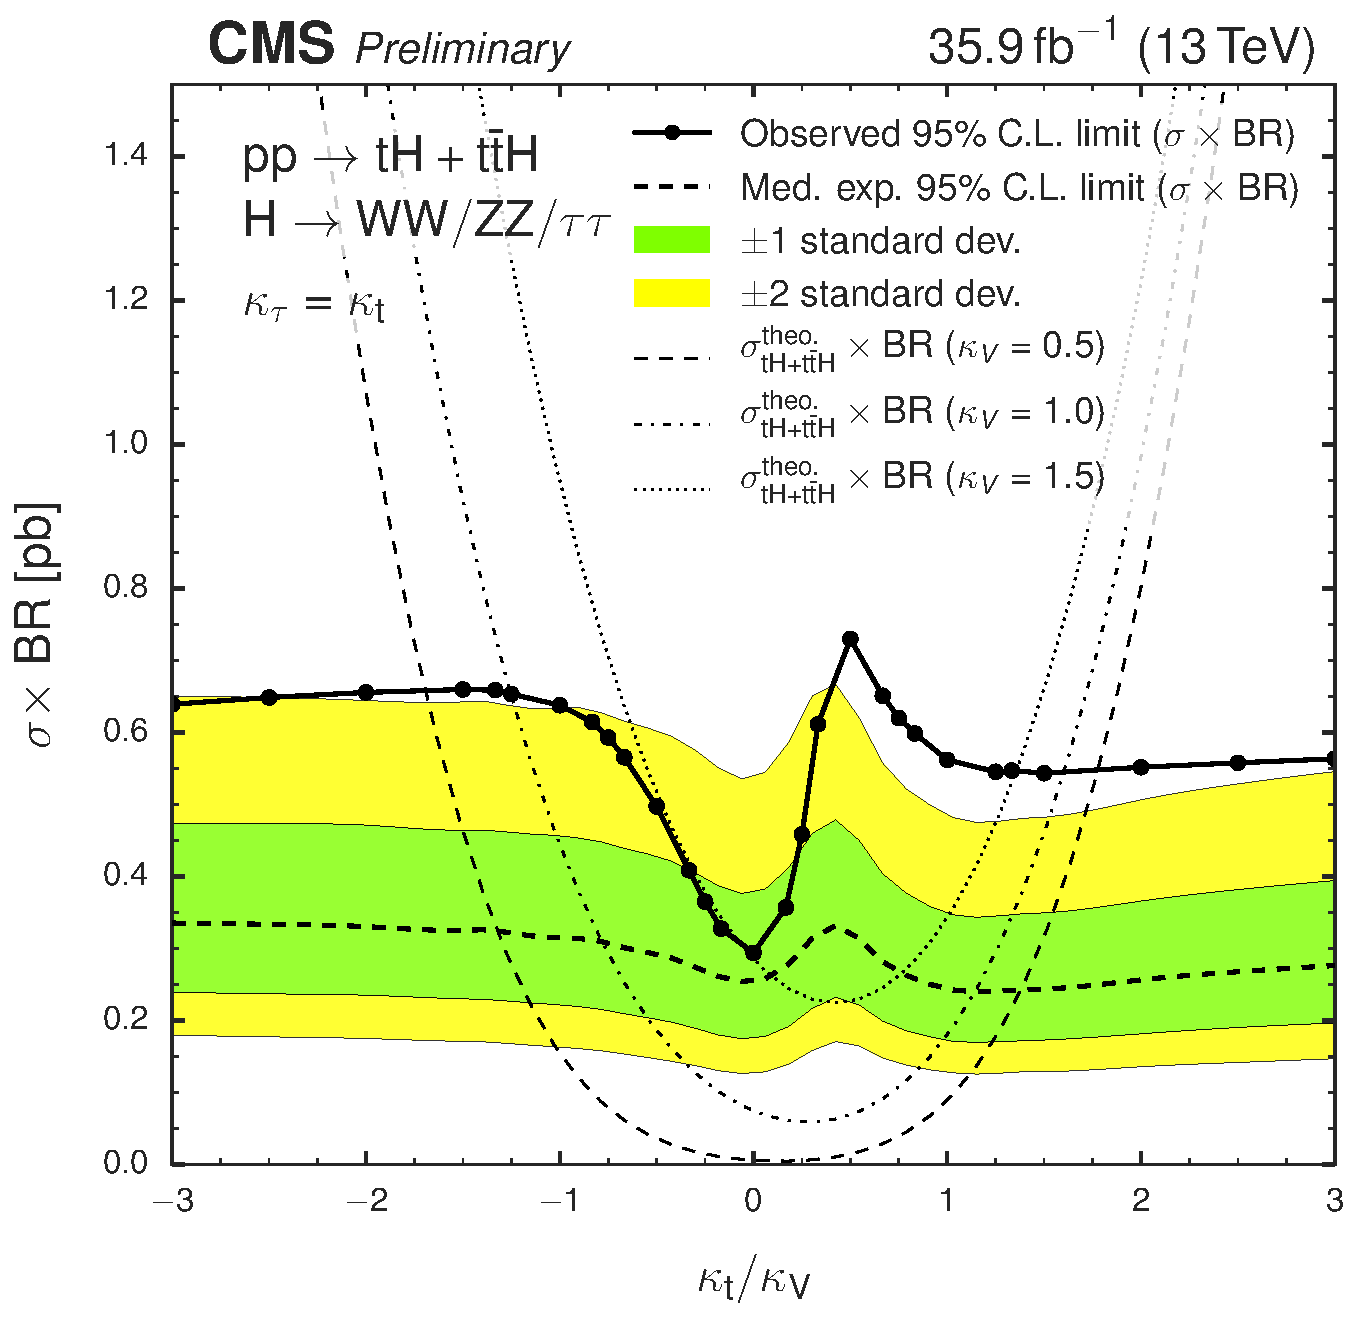
\includegraphics[width=0.48\textwidth]{figures/limits/xs_limits_K6_split_cv.pdf}\\
 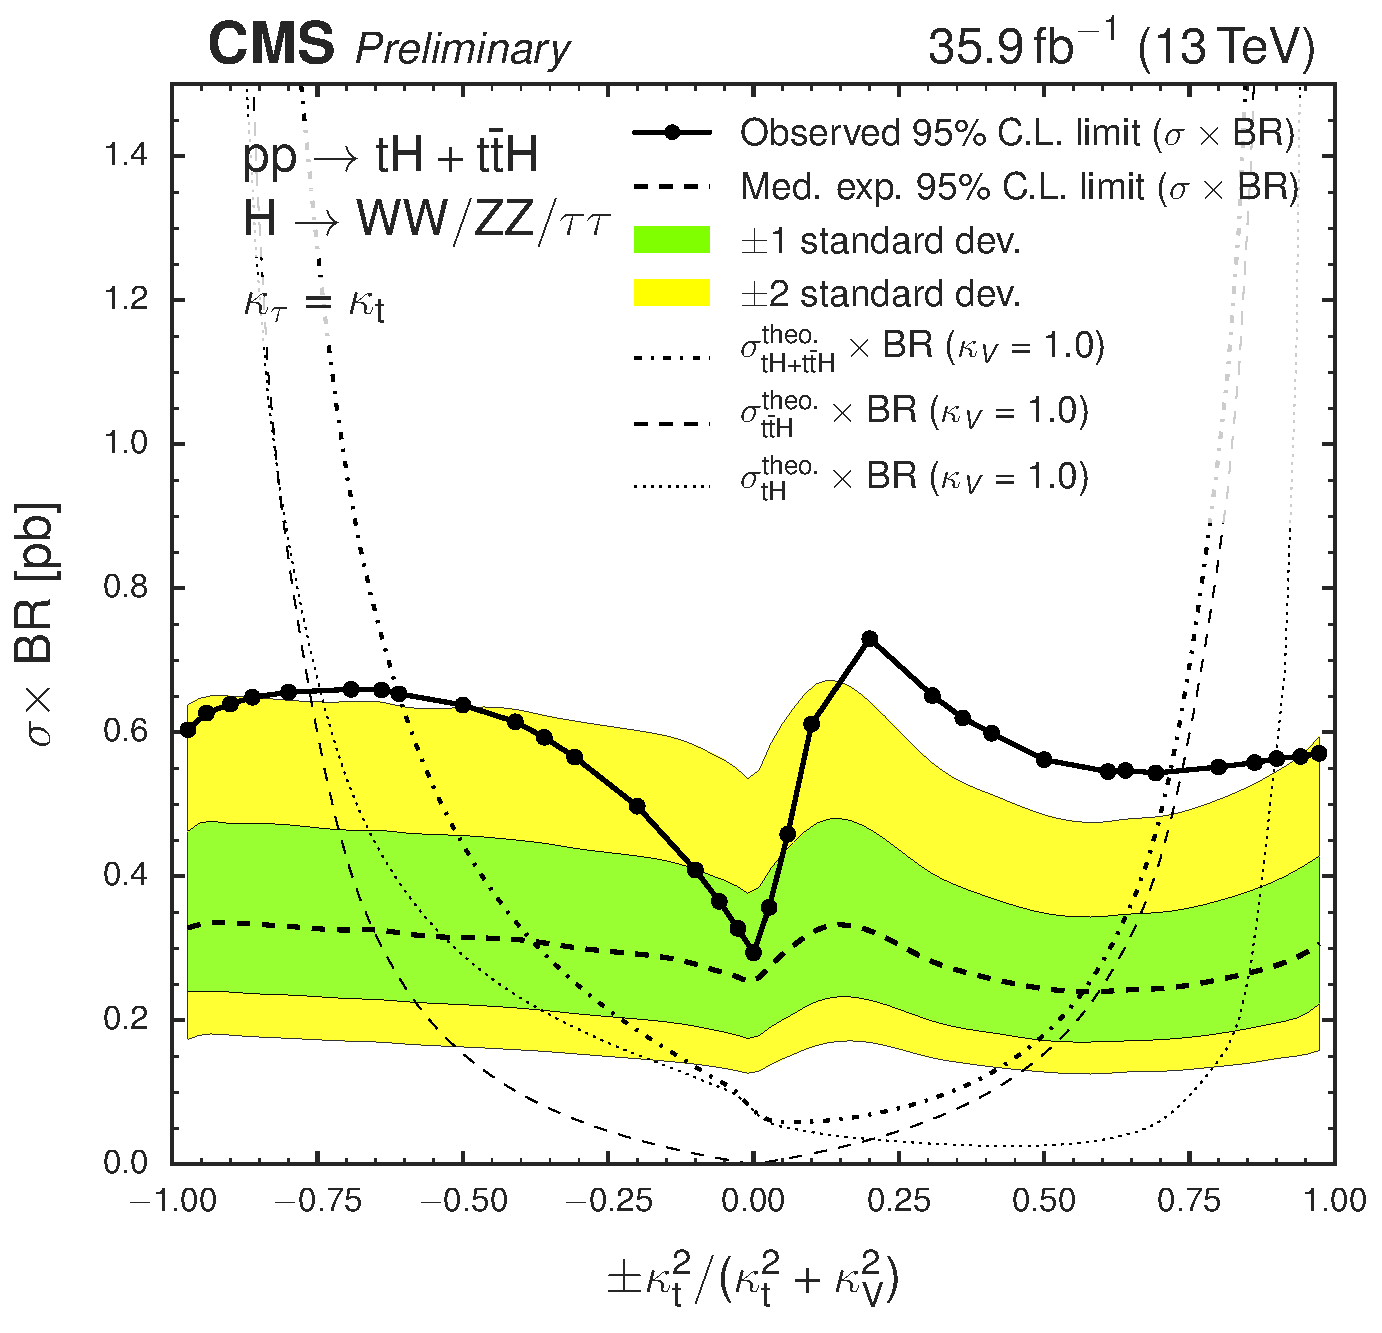
\includegraphics[width=0.48\textwidth]{figures/limits/xs_limits_K6_alpha.pdf}
 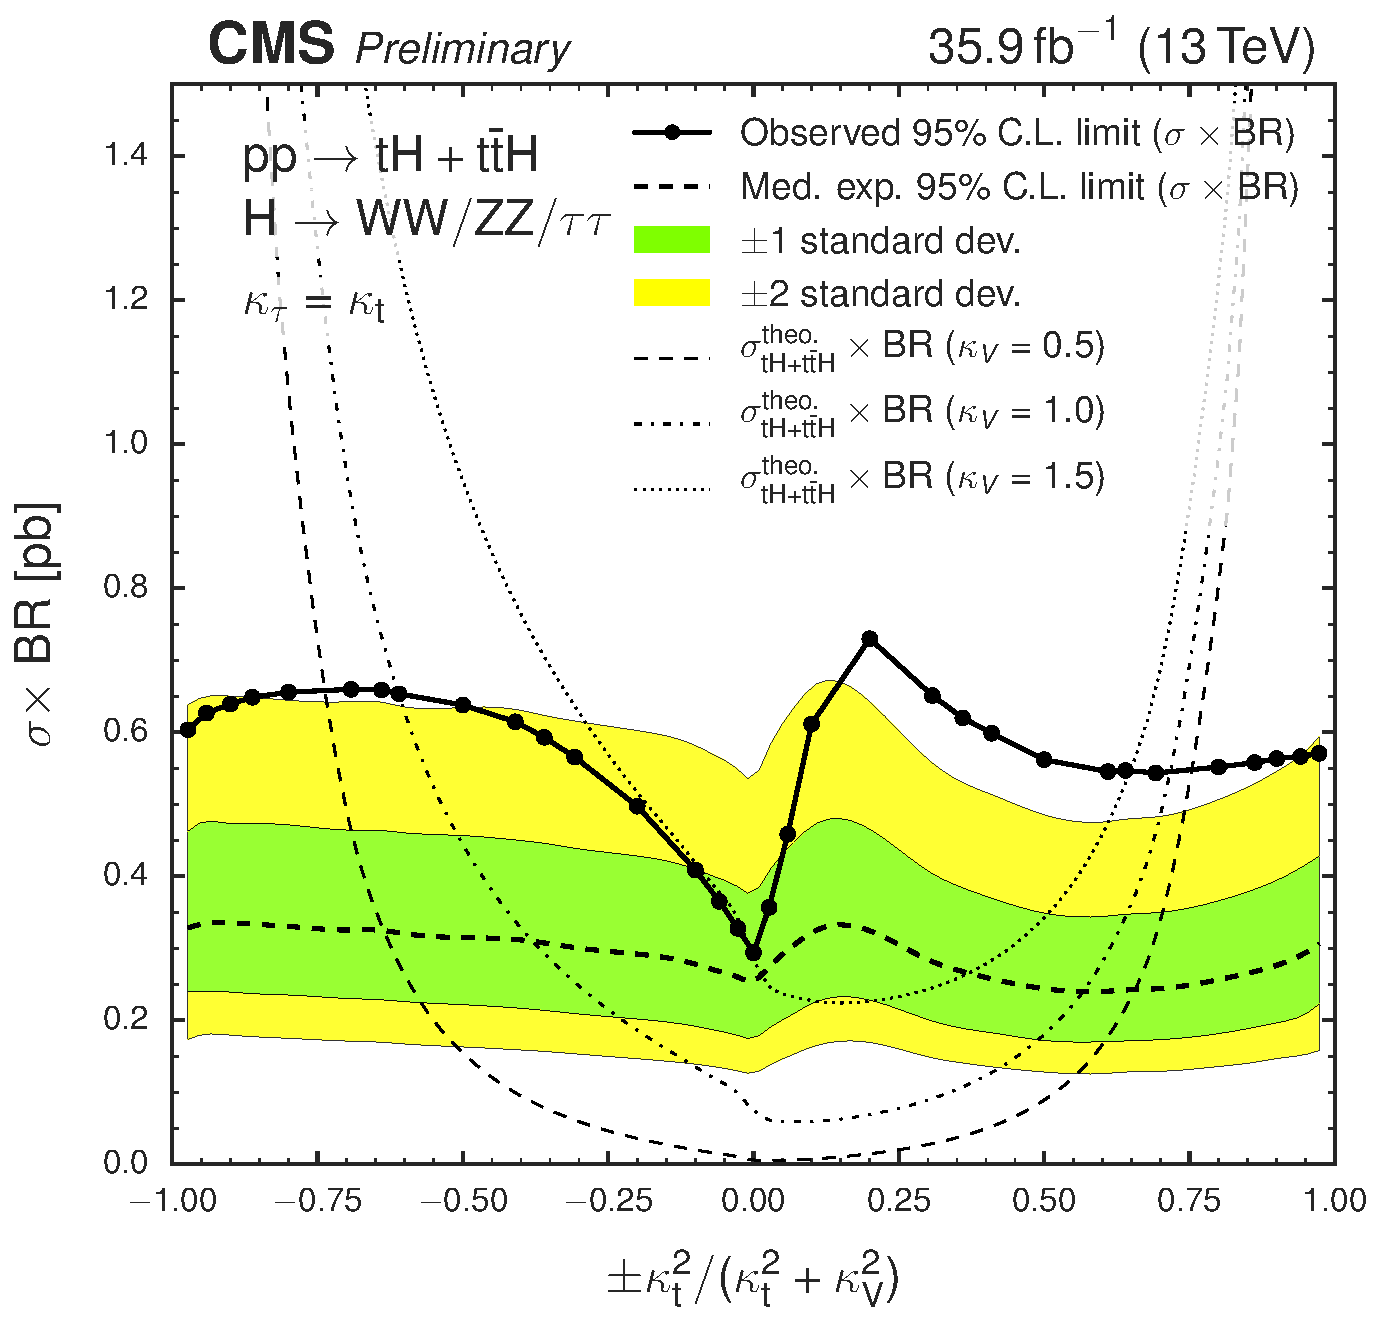
\includegraphics[width=0.48\textwidth]{figures/limits/xs_limits_K6_alpha_split_cv.pdf}
\caption{Expected (from background-only) and observed asymptotic limits on the combined $\tH+\ttH$ cross section times modified BR as a function of $\Ct/\CV$ (top) and $\mathrm{sign}(\Ct/\CV)\times\frac{\Ct^2}{(\Ct^2+\CV^2)}$ (bottom) for the combination of three lepton channel, \mumu, and \emu\ channel.}
\label{fig:xs_limits_cv}
\end{figure}

\begin{figure} [!h]
 \centering
 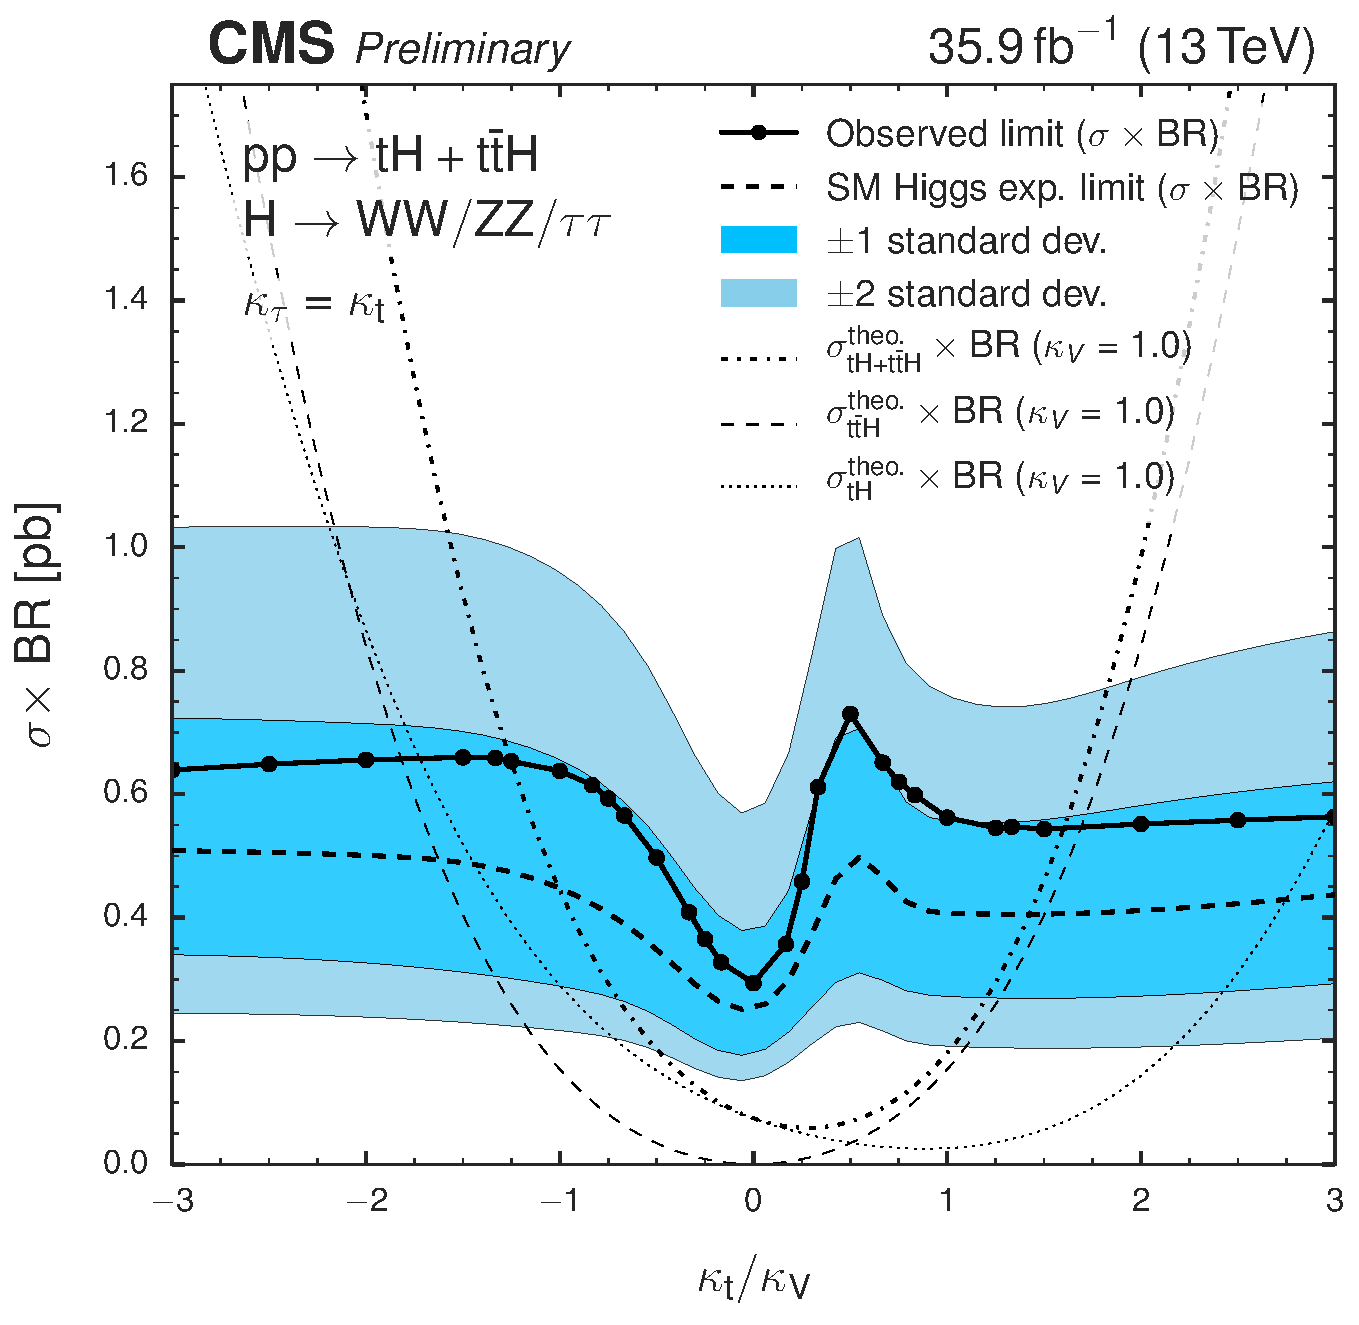
\includegraphics[width=0.48\textwidth]{figures/limits/xs_limits_K6_smexp.pdf}
 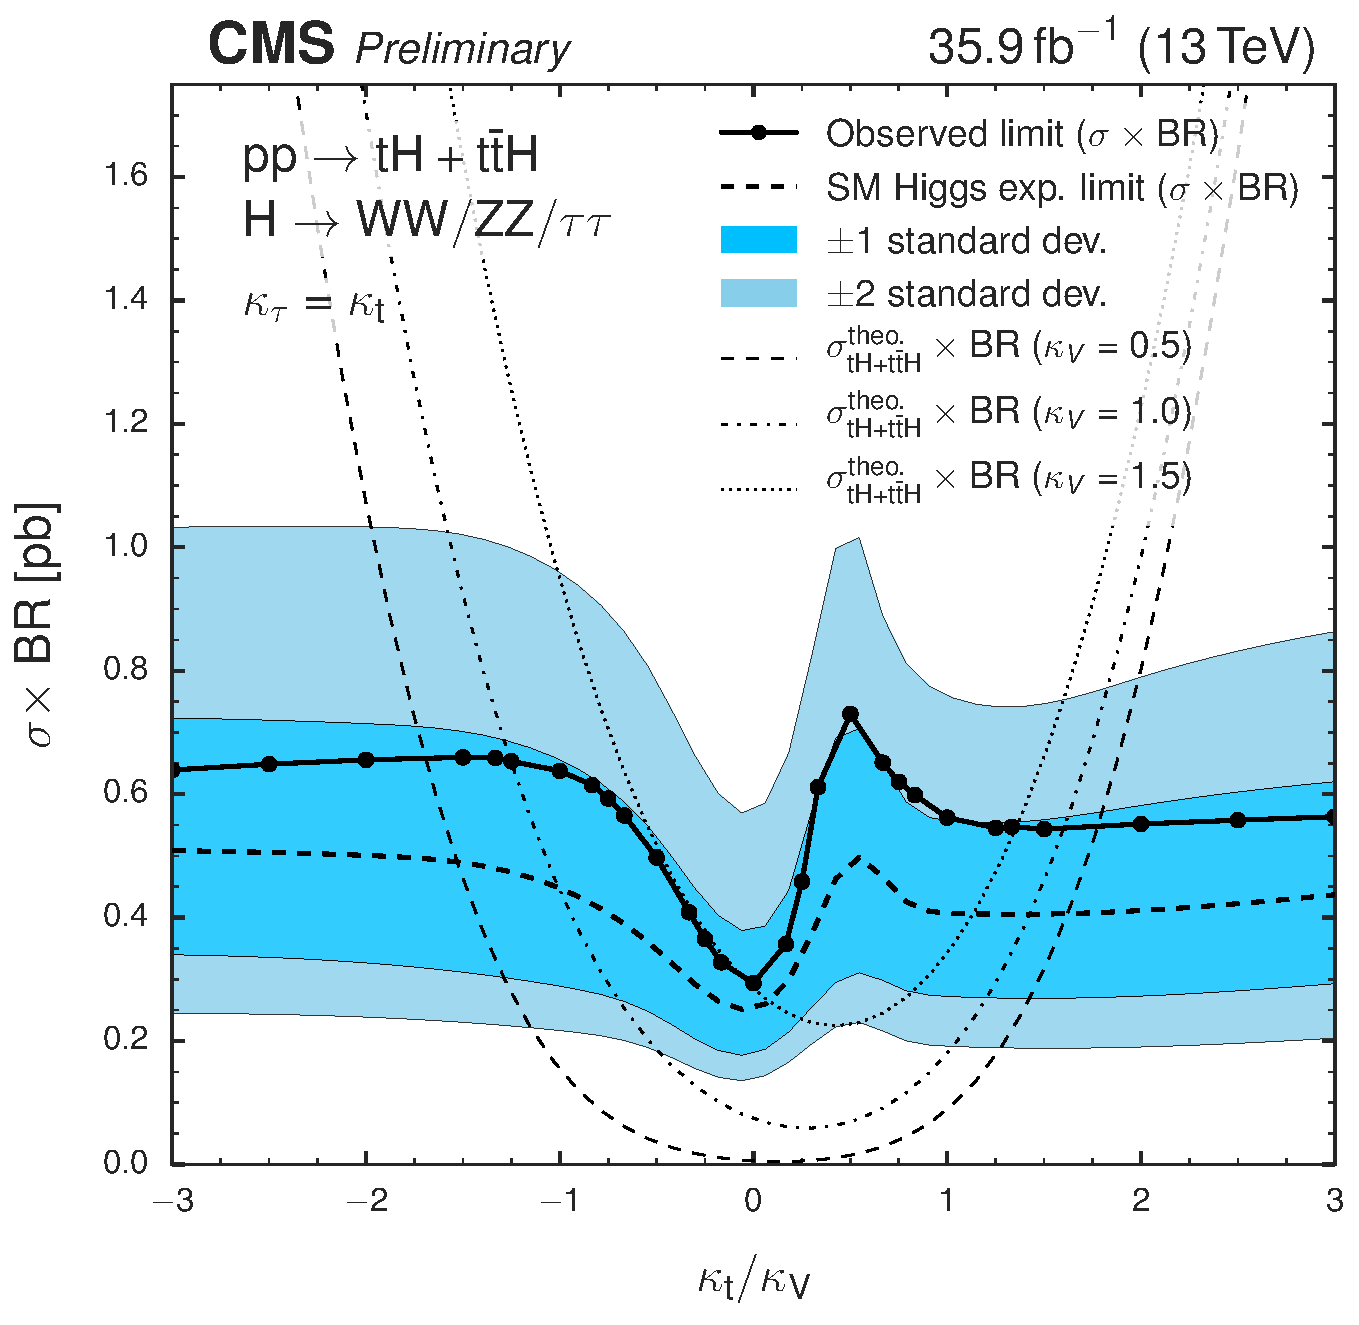
\includegraphics[width=0.48\textwidth]{figures/limits/xs_limits_K6_smexp_split_cv.pdf}\\
 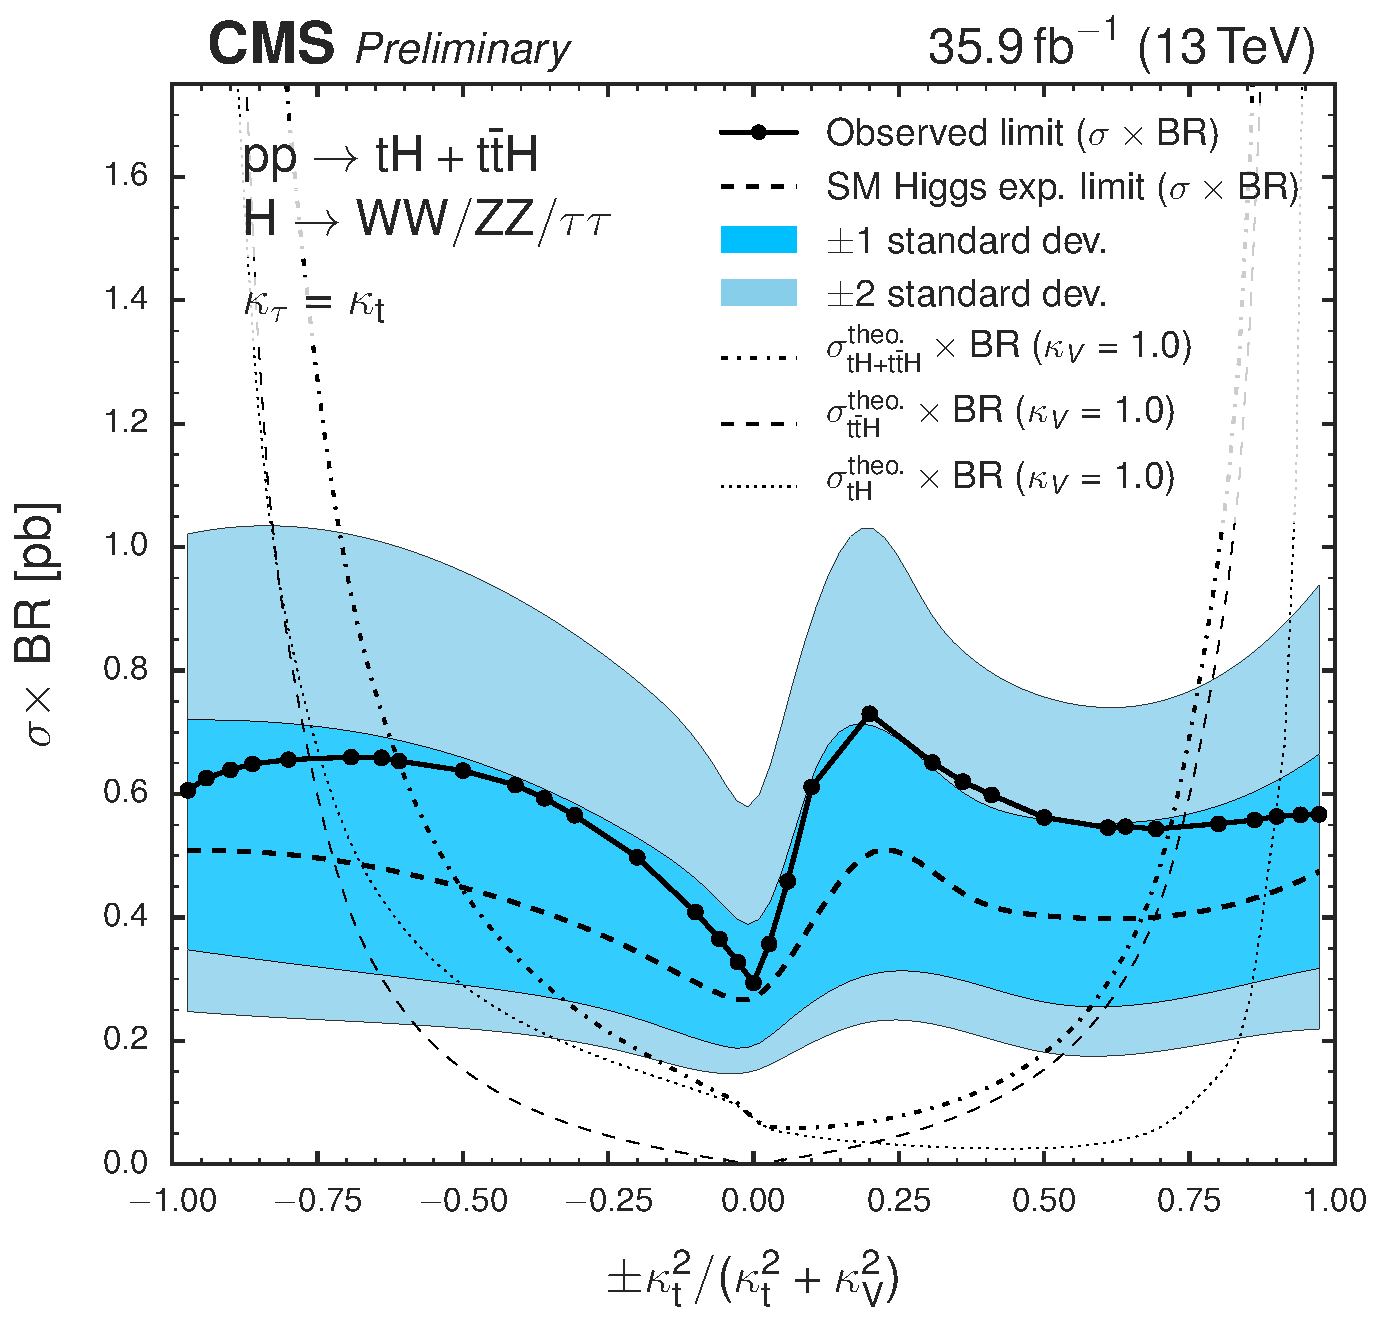
\includegraphics[width=0.48\textwidth]{figures/limits/xs_limits_K6_alpha_smexp.pdf}
 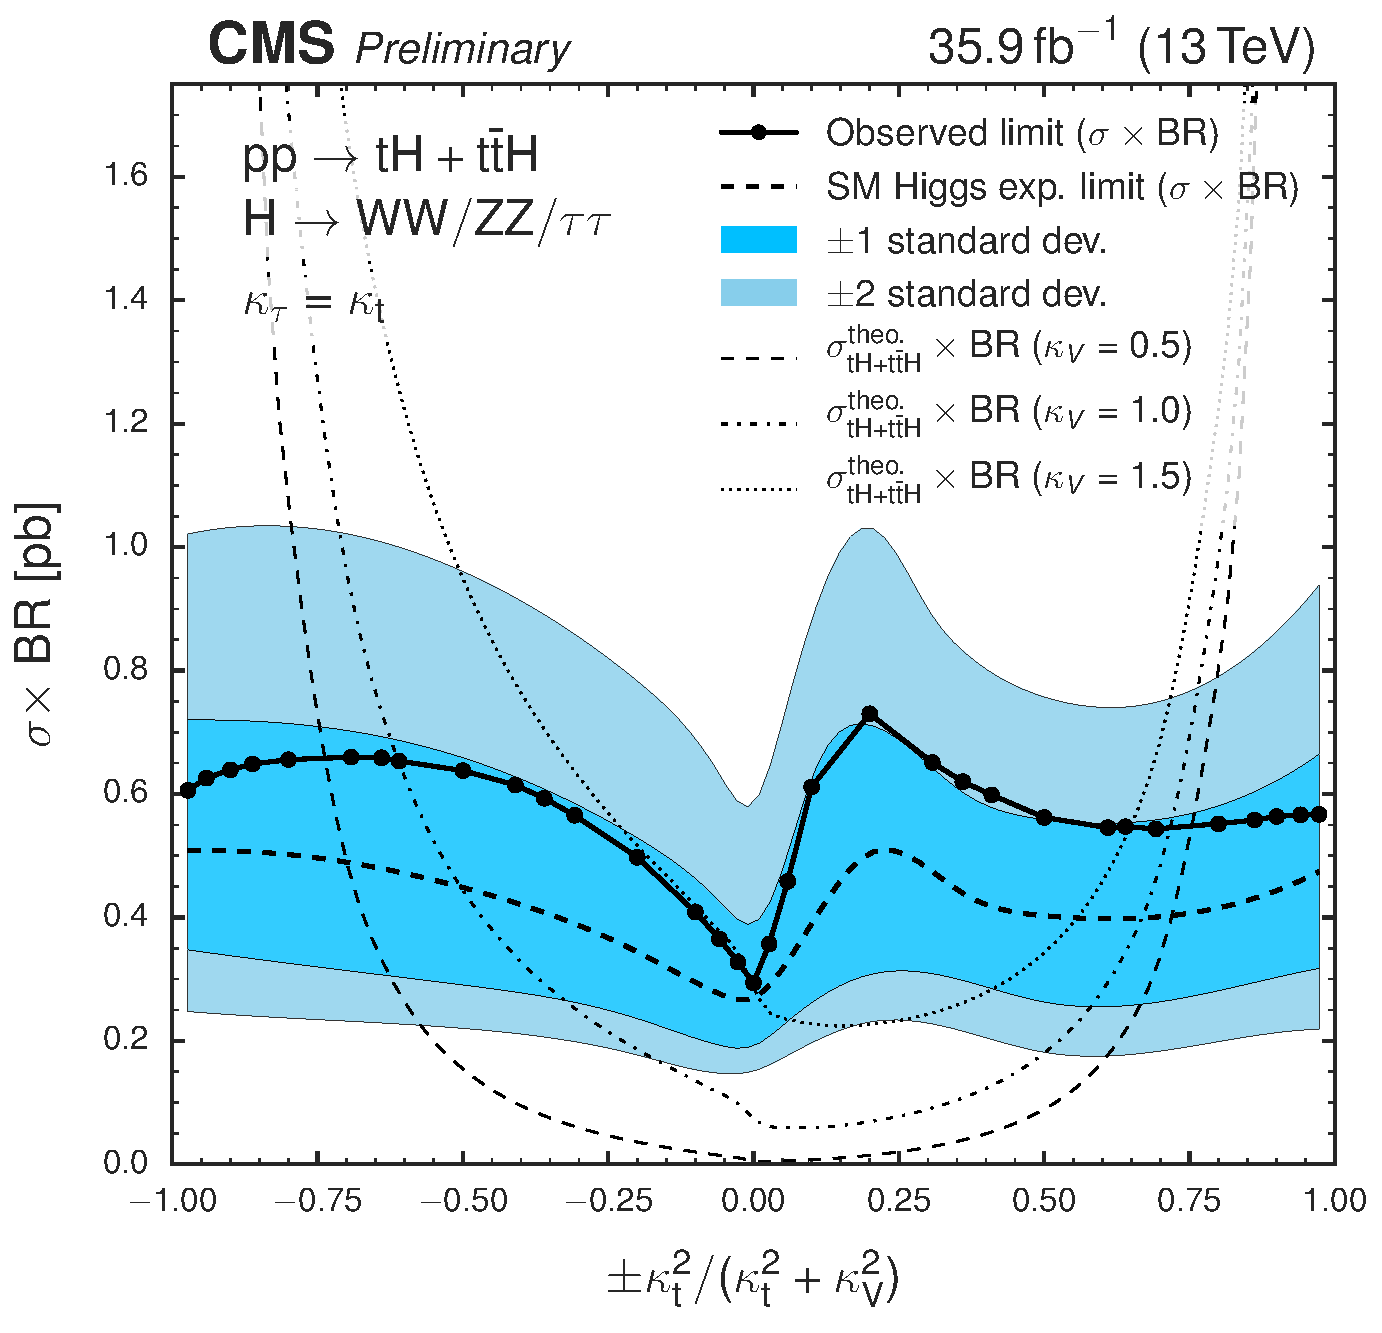
\includegraphics[width=0.48\textwidth]{figures/limits/xs_limits_K6_alpha_smexp_split_cv.pdf}
\caption{As Fig.~\ref{fig:xs_limits_cv} but calculating the expected limit on an Asimov dataset that includes SM-like \ttH\ and \tH\ signals.}
\label{fig:xs_limits_cv_smexp}
\end{figure}

\begin{figure} [!h]
 \centering
 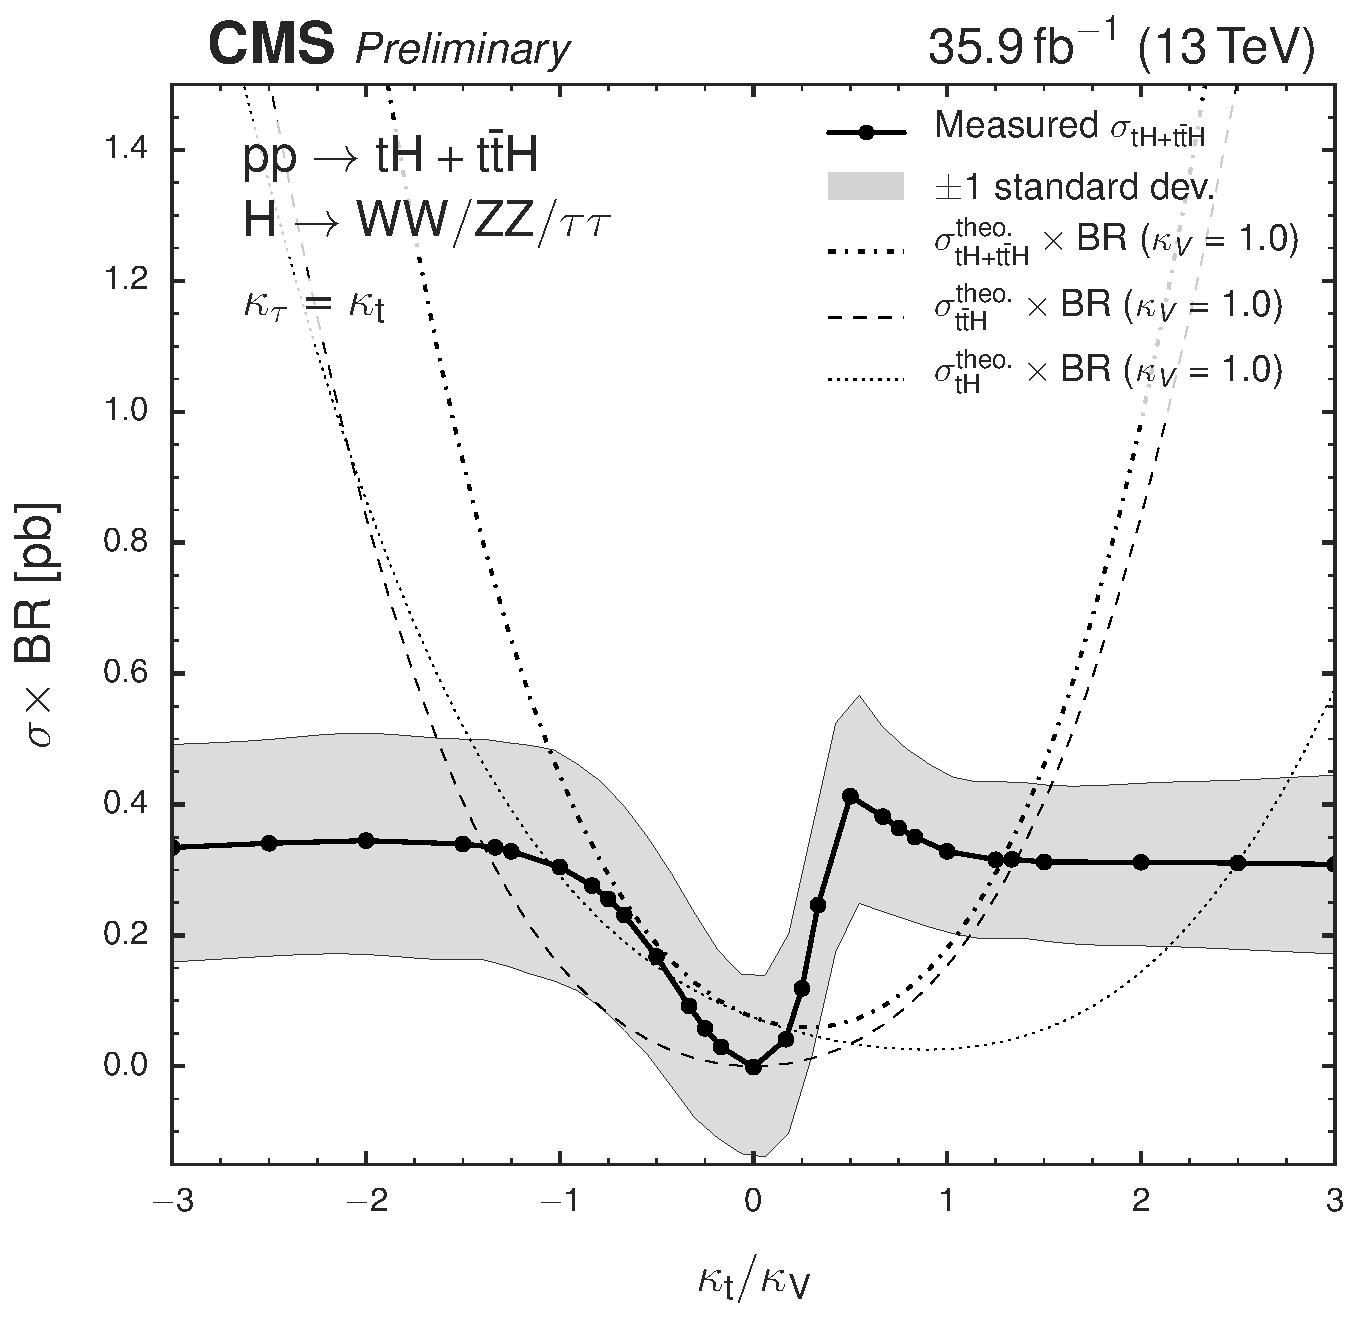
\includegraphics[width=0.48\textwidth]{figures/limits/xs_fits_K6.pdf}
 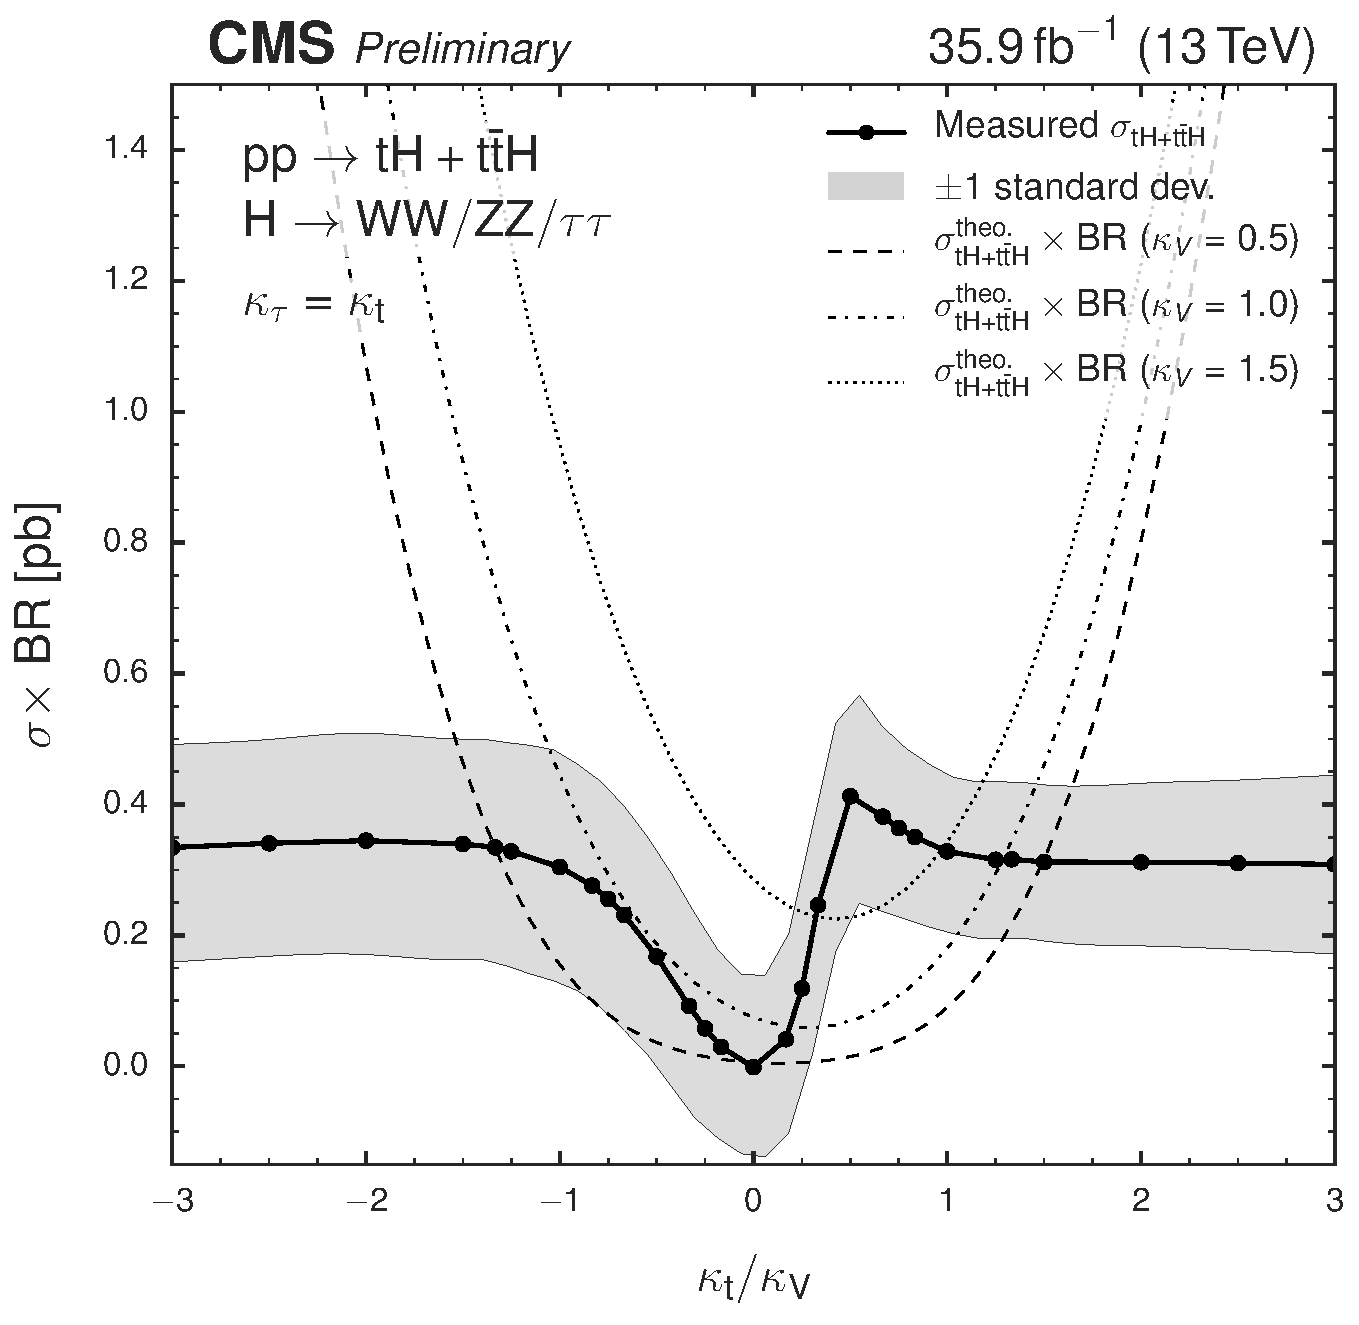
\includegraphics[width=0.48\textwidth]{figures/limits/xs_fits_K6_split_cv.pdf}\\
 \includegraphics[width=0.48\textwidth]{figures/limits/xs_fits_K6_alpha.pdf}
 \includegraphics[width=0.48\textwidth]{figures/limits/xs_fits_K6_alpha_split_cv.pdf}
\caption{Best fit values of the combined $\tH+\ttH$ cross section times modified BR as a function of $\Ct/\CV$ (top) and $\mathrm{sign}(\Ct/\CV)\times\frac{\Ct^2}{(\Ct^2+\CV^2)}$ (bottom) for the combination of three lepton channel, \mumu, and \emu\ channel.}
\label{fig:xs_fits_cv}
\end{figure}


\begin{figure} [!h]
 \centering
 \includegraphics[width=0.48\textwidth]{figures/significances/significances.pdf} \\
 \includegraphics[width=0.48\textwidth]{figures/significances/significances_alpha.pdf}
\caption{Observed and a priori expected significance of the fit result (in a background-only hypothesis) as a function of $\Ct/\CV$ (top) and \ft\ (bottom) for the combination of three lepton channel, \mumu, and \emu\ channel.}
\label{fig:significances}
\end{figure}

% \begin{figure} [!h] %% FIXME: Put in appendix
%  \centering
%  \includegraphics[width=0.48\textwidth]{figures/limits/limits_comb3_K4_cv_1p0.pdf}
%  \includegraphics[width=0.48\textwidth]{figures/limits/limits_comb3_K5_cv_1p0.pdf}\\
%  \includegraphics[width=0.48\textwidth]{figures/limits/limits_comb3_K4_cv_1p5.pdf}
%  \includegraphics[width=0.48\textwidth]{figures/limits/limits_comb3_K5_cv_1p5.pdf}\\
%  \includegraphics[width=0.48\textwidth]{figures/limits/limits_comb3_K4_cv_0p5.pdf}
%  \includegraphics[width=0.48\textwidth]{figures/limits/limits_comb3_K5_cv_0p5.pdf}
% \caption{Expected asymptotic limits on the combined $\tH+\ttH$ signal strength as a function of \Ct\ for $\CV=1.0$, $\CV=1.5$, $\CV=0.5$ (top to bottom) for the combination of three lepton channel, \mumu, and \emu\ channel, for the resolved model (left, with modified $\PH\to\gamma\gamma/\Z\gamma/\Pg\Pg$ branching ratios), and the unresolved model (right, with unmodified overall Higgs decay width.). (Note that the slight dip at $\Ct=0,\CV=0.5$ is the result of a bug, and not physical.)}
% \label{fig:r_limits_cv}
% \end{figure}

\begin{figure} [!h]
 \centering
 \includegraphics[width=0.8\textwidth]{figures/limits/impacts/impacts1.pdf}\\
 \includegraphics[width=0.8\textwidth]{figures/limits/impacts/impacts2.pdf}\\
\caption{Post-fit pulls and impacts of the 40 nuisance parameters with largest impacts for the fit on the observed data, for the $\Ct/\CV=-1.0$ hypothesis.}
\label{fig:impacts}
\end{figure}

\begin{figure} [!h]
 \centering
 \includegraphics[width=0.8\textwidth]{figures/limits/impacts/sm/impacts1.pdf}\\
 \includegraphics[width=0.8\textwidth]{figures/limits/impacts/sm/impacts2.pdf}\\
\caption{Post-fit pulls and impacts of the 40 nuisance parameters with largest impacts for the fit on the observed data, for the standard model ($\Ct/\CV=1.0$) hypothesis.}
\label{fig:impacts_sm}
\end{figure}

\begin{figure} [!h]
 \centering
 \includegraphics[width=0.8\textwidth]{figures/limits/impacts/asimov/impacts1.pdf}\\
 \includegraphics[width=0.8\textwidth]{figures/limits/impacts/asimov/impacts2.pdf}\\
\caption{Post-fit pulls and impacts of the 40 nuisance parameters with largest impacts for a fit to the Asimov dataset with fixed signal strength, for the $\Ct/\CV=-1.0$ hypothesis.}
\label{fig:impacts_asimov}
\end{figure}
